% !TEX encoding = UTF-8 Unicode
% !TEX TS-program = pdflatex

% toptesti document class
\documentclass[%
    a4paper, % not needed, by default it is a4paper, or also b5paper can be used
    corpo=12pt, % dimension of basic font
    % oneside is generally the way to go
    twoside, % two side optimizes for two-face printing, having chapters open on the right (aka odd numbers), if you don't want blank pages put oneside here
    stile=standard,
    %evenboxes, % not needed, to put supervisors and candidate at the same level
    tipotesi=magistrale,
    numerazioneromana, % roman numbering for appendixes and preambles, up to Table of Contents
    openright, % to force opening on the right for double-sided printing
    cucitura=7mm, % for printing, 7mm should be enough
    %dvipsnames, % for compatibility with xcolor, it does not work
]{toptesi}

%%%%%%%%%%%%%%%%%%%%%%%%%%%%%%%%%%%%%%%%%%%%%%%%%%%%
\usepackage[english]{babel}
\usepackage[utf8]{inputenc}
\usepackage[T1]{fontenc}
\usepackage{lmodern}

\usepackage{hyperref} % must be loaded before glossaries-extra

% bibliography
\usepackage[hyperref=true,backref=true,backend=biber,maxbibnames=9,maxcitenames=2,style=numeric,citestyle=numeric-comp,sorting=none,urldate=long]{biblatex} % hyperref uses links, backref goes back to citations, uses biber as backend, with 9 names at most in bibliography and 2 in citations, citing using numbers, and sorting in citation order
% sorting can be also ydnt for year descending, name, title or ynt for ascending year

\usepackage{adjustbox} % to resize boxes by keeping the same aspect ratio
\usepackage{algorithm} % algorithm environment
%\PassOptionsToPackage{noend}{algpseudocode}% comment out if want end's to show
\usepackage{algpseudocode} % improved pseudo-code
\usepackage{amsfonts}               %  AMS mathematical fonts
\usepackage{amsmath}
\usepackage{amssymb}                %  AMS mathematical symbols
\usepackage{amsthm}
\theoremstyle{definition}
\newtheorem{definition}{Definition}[section]
\theoremstyle{remark}
\newtheorem*{remark}{Remark}
\theoremstyle{definition}
\newtheorem{theorem}{Theorem}[section]
\usepackage{bm}                     %  black/bold mathematical symbols
\usepackage{booktabs}               %  better tables
\usepackage{calc}
\usepackage[labelfont=bf]{caption} % font=footnotesize % to have reduced caption font size
\usepackage{chronosys} % to draw timelines
\usepackage{csquotes}
\usepackage{enumitem} %left align the bulleted points
\usepackage{geometry}
\usepackage[%
    toc, % puts the link in the ToC record, % to use bib2gls
    abbreviations, % to load abbreviations / acronyms
    symbols, % to load symbols
    nonumberlist, % to avoid printing the numbers of the references in the acronyms page
    style=index, % in-line acronyms
]{glossaries-extra}
\usepackage{graphicx}               %  post-script images
%\usepackage{iwona} % extra fonts, substitute standard ones
\usepackage{listings} % to insert formatted code
\usepackage{lipsum} % for lorem ipsum text, not needed in the real work
\usepackage{makecell} % to change dimensions of cells, for math cases
\usepackage{mathtools} % for additional commands
\DeclarePairedDelimiter\ceil{\lceil}{\rceil}
\DeclarePairedDelimiter\floor{\lfloor}{\rfloor}
\usepackage{mfirstuc} % to have capitalization capabilities
\usepackage[final]{microtype}      % microtypography, final lets latex use it also in bibliography
\usepackage{multirow} % to allow for cells covering more than 1 row in tables
\newcommand{\STAB}[1]{\begin{tabular}{@{}c@{}}#1\end{tabular}}
\usepackage{nicefrac}       % compact symbols for 1/2, etc.
%\usepackage[lofdepth,lotdepth]{subfig}
\usepackage{ragged2e} % for justifying text
\usepackage{scrextend} % for multiple references to the same footnote
\usepackage{siunitx} % support for SI units of measurement and number typesetting
\usepackage[figuresright]{rotating}
%\usepackage{subfig}
\usepackage{subcaption} %  subfigure compatibility
\usepackage{svg} % for svg support, works only if inkscape is installed, default for Overleaf v2
\usepackage{tabularx} % equal-width columns in tables
\usepackage{textcomp} % extra fonts and symbols
\usepackage{url}            % simple URL typesetting
\usepackage{verbatim} % for extended verbatim support
\usepackage{xcolor} % to define colors and use standard CSS names add dvipsnames as option, but it clashes with xcolor loaded in toptesi, pay attention that if it goes in conflict with tikz/beamer, simply use \documentclass[usenames,dvipsnames]{beamer}, along with other custom options when defining the document class
\usepackage{xpatch}






% begin vertical rule patch for algorithmicx (http://tex.stackexchange.com/questions/144840/vertical-loop-block-lines-in-algorithmicx-with-noend-option)
\makeatletter
% start with some helper code
% This is the vertical rule that is inserted
\newcommand*{\algrule}[1][\algorithmicindent]{\makebox[#1][l]{\hspace*{.5em}\vrule height .75\baselineskip depth .25\baselineskip}}%

\newcount\ALG@printindent@tempcnta
\def\ALG@printindent{%
    \ifnum \theALG@nested>0% is there anything to print
        \ifx\ALG@text\ALG@x@notext% is this an end group without any text?
            % do nothing
            \addvspace{-3pt}% FUDGE for cases where no text is shown, to make the rules line up
        \else
            \unskip
            % draw a rule for each indent level
            \ALG@printindent@tempcnta=1
            \loop
                \algrule[\csname ALG@ind@\the\ALG@printindent@tempcnta\endcsname]%
                \advance \ALG@printindent@tempcnta 1
            \ifnum \ALG@printindent@tempcnta<\numexpr\theALG@nested+1\relax% can't do <=, so add one to RHS and use < instead
            \repeat
        \fi
    \fi
    }%
\usepackage{etoolbox}
% the following line injects our new indent handling code in place of the default spacing
\patchcmd{\ALG@doentity}{\noindent\hskip\ALG@tlm}{\ALG@printindent}{}{\errmessage{failed to patch}}
\makeatother
% end vertical rule patch for algorithmicx



\DeclareMathOperator*{\argmax}{arg\,max}
\DeclareMathOperator*{\argmin}{arg\,min}
\DeclareMathOperator*{\argsup}{arg\,sup}
\DeclareMathOperator*{\arginf}{arg\,inf}
\DeclarePairedDelimiterX{\dotp}[2]{\langle}{\rangle}{#1, #2}



\newcommand*{\inlineimg}[1]{%
    \raisebox{-.3\baselineskip}{%
        \includegraphics[
        height=\baselineskip,
        width=\baselineskip,
        keepaspectratio,
        ]{#1}%
    }%
}



% for not letting footnotes break in two pages
\interfootnotelinepenalty=1000000





%%%%%%%%%% NEW GLOSSARY STYLE
\newglossarystyle{myglosses}{
    \renewenvironment{theglossary}{
        \longtable{r l}
    }{
        \endlongtable
    }
    \renewcommand*{\glossaryheader}{}
    \renewcommand*{\glsgroupheading}[1]{}
    \renewcommand*{\glsgroupskip}{}
    \renewcommand*{\glsclearpage}{} 

     % set how each entry should appear:
      \renewcommand*{\glossentry}[2]{
        \glstarget{##1}{\textsc{\glossentryname{##1}}}
        &
        \glossentrydesc{##1} \\
    }
    \renewcommand*{\subglossentry}[3]{%
        \glossentry{##2}{##3}
    }
}

% configuration for glossaries
% convert and load converted glossaries in .tex ,format from .bib
\setabbreviationstyle{long-short-desc} % style before loading resources
% this command sets the style to title for long names of acronyms only in the glossary description, leading to capitalized first-letter for all words
%\newglossary*{abbreviation}{Acronyms} % to change the name of this glossary for acronyms



% setup for hyperref
\hypersetup{%
    pdfpagemode={UseOutlines},
    bookmarksopen,
    pdfstartview={FitH},
    colorlinks,
    linkcolor={black}, % it is suggested to keep them black, since when printing it it costs per page, and if they have color it's twice the price per page
    citecolor={black},
    urlcolor={black}
  }
%

% setup for svg
\svgsetup{%
    inkscapeformat=pdf, % to force usage of PDF
    inkscapelatex=false, % to disable latex rendering of text, produces errors
}

% setup for siunitx, it does not work in the summary
\sisetup{%
    detect-all, % to use the same font as for writing when using \num
    mode=text, % to allow it to work also in math mode
    group-separator = {,}, % separator for number grouping
    group-minimum-digits = 3, % minimum number of digits a number must have to be grouped in 3-digit groups
}

% listings colours
\definecolor{rulecolor}{rgb}{0,0,0}
\definecolor{commentcolor}{rgb}{0,0.6,0}
\definecolor{linenumbercolor}{rgb}{0.5,0.5,0.5}
\definecolor{keywordcolor}{rgb}{0,0,0.95}
\definecolor{backcolor}{rgb}{1,1,1}%{0.95,0.95,0.92}
\definecolor{stringcolor}{rgb}{0.58,0,0.82}

% setup for lstlisting
\lstset{ %
	backgroundcolor=\color{backcolor},   % choose the background color; you must add \usepackage{color} or \usepackage{xcolor}; should come as last argument
	basicstyle=\footnotesize,        % the size of the fonts that are used for the code
	breakatwhitespace=false,         % sets if automatic breaks should only happen at whitespace
	breaklines=true,                 % sets automatic line breaking
	captionpos=t,                    % sets the caption-position to bottom
	commentstyle=\color{commentcolor},    % comment style
	extendedchars=true,              % lets you use non-ASCII characters; for 8-bits encodings only, does not work with UTF-8
	frame=single,	                   % adds a frame around the code
	keepspaces=true,                 % keeps spaces in text, useful for keeping indentation of code (possibly needs columns=flexible)
	keywordstyle=\color{keywordcolor},       % keyword style
	%language=VHDL,                 % the language of the code
	numbers=left,                    % where to put the line-numbers; possible values are (none, left, right)
	numbersep=5pt,                   % how far the line-numbers are from the code
	numberstyle=\tiny\color{linenumbercolor}, % the style that is used for the line-numbers
	rulecolor=\color{rulecolor},         % if not set, the frame-color may be changed on line-breaks within not-black text (e.g. comments (green here))
	showspaces=false,                % show spaces everywhere adding particular underscores; it overrides 'showstringspaces'
	showstringspaces=false,          % underline spaces within strings only
	showtabs=false,                  % show tabs within strings adding particular underscores
	stepnumber=1,                    % the step between two line-numbers. If it's 1, each line will be numbered
	stringstyle=\color{stringcolor},     % string literal style
	tabsize=4,	                   % sets default tabsize to 2 spaces
	title=\lstname,                   % show the filename of files included with \lstinputlisting; also try caption instead of title
	inputencoding=utf8,
	literate=
	{á}{{\'a}}1 {é}{{\'e}}1 {í}{{\'i}}1 {ó}{{\'o}}1 {ú}{{\'u}}1
	{Á}{{\'A}}1 {É}{{\'E}}1 {Í}{{\'I}}1 {Ó}{{\'O}}1 {Ú}{{\'U}}1
	{à}{{\`a}}1 {è}{{\`e}}1 {ì}{{\`i}}1 {ò}{{\`o}}1 {ù}{{\`u}}1
	{À}{{\`A}}1 {È}{{\'E}}1 {Ì}{{\`I}}1 {Ò}{{\`O}}1 {Ù}{{\`U}}1
	{ä}{{\"a}}1 {ë}{{\"e}}1 {ï}{{\"i}}1 {ö}{{\"o}}1 {ü}{{\"u}}1
	{Ä}{{\"A}}1 {Ë}{{\"E}}1 {Ï}{{\"I}}1 {Ö}{{\"O}}1 {Ü}{{\"U}}1
	{â}{{\^a}}1 {ê}{{\^e}}1 {î}{{\^i}}1 {ô}{{\^o}}1 {û}{{\^u}}1
	{Â}{{\^A}}1 {Ê}{{\^E}}1 {Î}{{\^I}}1 {Ô}{{\^O}}1 {Û}{{\^U}}1
	{œ}{{\oe}}1 {Œ}{{\OE}}1 {æ}{{\ae}}1 {Æ}{{\AE}}1 {ß}{{\ss}}1
	{ű}{{\H{u}}}1 {Ű}{{\H{U}}}1 {ő}{{\H{o}}}1 {Ő}{{\H{O}}}1
	{ç}{{\c c}}1 {Ç}{{\c C}}1 {ø}{{\o}}1 {å}{{\r a}}1 {Å}{{\r A}}1
	{€}{{\euro}}1 {£}{{\pounds}}1 {«}{{\guillemotleft}}1
	{»}{{\guillemotright}}1 {ñ}{{\~n}}1 {Ñ}{{\~N}}1 {¿}{{?`}}1
}


% biblatex setup
% generally 9000 is ok, if higher than 10000 it's bad
% If you want to break on URL numbers
\setcounter{biburlnumpenalty}{9000}
% If you want to break on URL lower case letters
\setcounter{biburllcpenalty}{9000}
% If you want to break on URL UPPER CASE letters
\setcounter{biburlucpenalty}{9000}



% how to change Contents to Table of Contents
\addto\captionsenglish{% Replace "english" with the language you use
  \renewcommand{\contentsname}%
    {Table of Contents}%
}

% to change the name of Abbreviations to Acronyms
% not needed if use use entry types and define those
% \renewcommand{\abbreviationsname}{Acronyms}

% to allow line comments in algorithms
\algnewcommand{\LineComment}[1]{\State \(\triangleright\) #1}

% to declare abs and norm
\DeclarePairedDelimiter\abs{\lvert}{\rvert}%
\DeclarePairedDelimiter\norm{\lVert}{\rVert}%

% Swap the definition of \abs* and \norm*, so that \abs
% and \norm resizes the size of the brackets, and the 
% starred version does not.
\makeatletter
\let\oldabs\abs
\def\abs{\@ifstar{\oldabs}{\oldabs*}}
%
\let\oldnorm\norm
\def\norm{\@ifstar{\oldnorm}{\oldnorm*}}
\makeatother



% custom commands for tables
\newcommand{\breakcell}[2][c]{%
  \begin{tabular}[#1]{@{}c@{}}#2\end{tabular}}
  
\newcommand{\breakcellleft}[2][l]{%
  \begin{tabular}[#1]{@{}l@{}}#2\end{tabular}}
  
\newcommand{\ra}[1]{\renewcommand{\arraystretch}{#1}}






% change this configuration with your info
% if you need fewer or more supervisors you have to change \relatore command by adding or removing lines in the table in toptesi_config
\newcommand{\thesistitle}{A novel procedure for real-time SOH estimation of EV battery packs based on Time Series Extrinsic Regression}
\newcommand{\thesisuniversitylogo}{images/logo/polito_logo} % choose your logo
\newcommand{\thesiscompanylogo}{images/logo/edison_logo} 
\newcommand{\thesiscandidatename}{Tommaso}
\newcommand{\thesiscandidatesurname}{Monopoli}
\newcommand{\thesissupervisoronetitle}{prof.}
\newcommand{\thesissupervisoronename}{Edoardo}
\newcommand{\thesissupervisoronesurname}{Patti}
\newcommand{\thesissupervisortwotitle}{prof.}
\newcommand{\thesissupervisortwoname}{Alessandro}
\newcommand{\thesissupervisortwosurname}{Aliberti}
\newcommand{\thesissupervisorthreetitle}{dott.}
\newcommand{\thesissupervisorthreename}{Raimondo}
\newcommand{\thesissupervisorthreesurname}{Gallo}
\newcommand{\thesissupervisorfourtitle}{dott.}
\newcommand{\thesissupervisorfourname}{Paolo}
\newcommand{\thesissupervisorfoursurname}{Tosco}
\newcommand{\thesisdate}{December 2022}
\newcommand{\thesiscourse}{Data Science and Engineering}
\newcommand{\thesisuniversity}{POLITECNICO DI TORINO}
\newcommand{\thesislevel}{Master} % master or bachelor
\newcommand{\thesiscandidatetext}{Candidate}
\newcommand{\thesissupervisortext}{Supervisors}


% fontsize is {size}{spacing}\family
\newcommand {\institutionfont}{\fontsize {22}{30}\scshape}
\newcommand {\divisionfont}{\fontsize {16}{20}\rmfamily}
\newcommand {\pretitlefont}{\fontsize {16}{16}\rmfamily}
\newcommand {\customtitlefont}{\fontsize {21}{28}\scshape}% {iwona}{bx}{n}}
\newcommand {\fixednamesfont}{\fontsize {14}{20}\mdseries}
\newcommand {\namesfont}{\fontsize {14}{20}\bfseries}
\newcommand {\footfont}{\fontsize {15}{18}\rmfamily}


\addbibresource{bibliography.bib}

% to load the glossaries, not needed if using bib2gls
%\input{glossaries.tex}
%\makeglossaries

\begin{document}

%\overfullrule=0.00001pt % latex shows a black bar for overfulls over this dimension

%\emergencystretch=1em % to allow some stretching in the lines to avoid overfull boxes, also in bibliography, eventually can be used only before bibliography or in the preamble for the whole document, not needed if using biblatex configuration in most cases


\ateneo{\thesisuniversity} % university name
\logosede[5cm]{\thesisuniversitylogo} % logo, square brackets contain the height

\titolo{\thesistitle} % title
%\sottotitolo{Metodo dei satelliti medicei} % subtitle

% place/remove a slash \\ to put the name on the following line or after Master Degree Course
\corsodilaurea{\thesiscourse} % course name


%~251197 % id number is not needed

\candidato{\thesiscandidatename~\textsc{\thesiscandidatesurname}} % candidate

% using tabular we can have more than 1 supervisor under the same column
\relatore{\tabular{@{}l}%
    \xmakefirstuc{\thesissupervisoronetitle}~\thesissupervisoronename~\textsc{\thesissupervisoronesurname}\\[0.4ex]
    \xmakefirstuc{\thesissupervisortwotitle}~\thesissupervisortwoname~\textsc{\thesissupervisortwosurname}\\[0.4ex]
    \xmakefirstuc{\thesissupervisorthreetitle}~\thesissupervisorthreename~\textsc{\thesissupervisorthreesurname}
    \endtabular}
%\terzorelatore{Ciao}

% in this way we have Academic Year without stile=classica, so without lines
%\sedutadilaurea{\textsc{Academic~Year} 2019-2020}% per la laurea magistrale
% for PoliTo there is only month year
\sedutadilaurea{\thesisdate}% per la laurea magistrale
% PhD
%\esamedidottorato{Novembre 1610}
%\ciclodidottorato{XV}

% offset for binding, the smaller the better
%\setbindingcorrection{3mm}


\english% or \italian (default)

\iflanguage{english}{%
	%\retrofrontespizio{This work is subject to the Creative Commons Licence}

	\CorsoDiLaureaIn{\thesislevel's Degree Course in\space}

	\TesiDiLaurea{\thesislevel's Degree Thesis}

	\InName{in}
	\CandidateName{\xmakefirstuc{\thesiscandidatetext}}% or Candidates
	\AdvisorName{\xmakefirstuc{\thesissupervisortext}}% or Supervisor
	%\TutorName{Tutor}
	%\NomeTutoreAziendale{Internship Tutor}

	%\NomePrimoTomo{First volume}
	%\NomeSecondoTomo{Second Volume}
	%\NomeTerzoTomo{Third Volume}
	%\NomeQuartoTomo{Fourth Volume}
}{}


% front page
% frontespizio can be used for the first page print
% while the custom-made frontpage can be used as hard-cover
% use pdfjoin or pdfseparate to extract or put together the pages if needed
%\frontespizio* % without star the logo is on top
\newgeometry{top=4cm,left=3cm,right=3cm,bottom=4cm,heightrounded}
\begin{titlepage}
\centering
%
{\institutionfont \textbf{\MakeUppercase{\thesisuniversity}} \par}
%
\vspace{\stretch{2}} % changing this number and the others changes the proportion
%
{\divisionfont \textbf{\thesislevel's Degree in \thesiscourse} \par}
%
\vspace{\stretch{3}}
%
\includegraphics[width=50mm]{\thesisuniversitylogo}
% \hspace{0.95cm}
% \raisebox{0.95cm}{\includegraphics[width=60mm]{\thesiscompanylogo}}\\
%
\vspace{\stretch{4}}
%
{\divisionfont \textbf{\thesislevel's Degree Thesis} \par}
%
\vspace{\stretch{3}}
%
{\customtitlefont \textbf{\thesistitle} \par}
%
\vspace{\stretch{10}}
%
\makebox[\textwidth]{\null\hfill\def\arraystretch{2}% % to change the spacing change this number
\begin{minipage}[t]{.375\textwidth}\raggedright
    \begin{adjustbox}{width={\textwidth},totalheight={\textheight},keepaspectratio} % with adjustbox it adapts to the lengths of the names, remove it if you want the same font dimension
    \begin{tabular}[t]{@{}l@{}}
        \fixednamesfont \textbf{\thesissupervisortext} \\
        \namesfont \xmakefirstuc{\thesissupervisoronetitle}~\thesissupervisoronename~\MakeUppercase{\thesissupervisoronesurname}\\
        \namesfont \xmakefirstuc{\thesissupervisortwotitle}~\thesissupervisortwoname~\MakeUppercase{\thesissupervisortwosurname}\\
        \namesfont \xmakefirstuc{\thesissupervisorthreetitle}~\thesissupervisorthreename~\MakeUppercase{\thesissupervisorthreesurname}\\
        \namesfont \xmakefirstuc{\thesissupervisorfourtitle}~\thesissupervisorfourname~\MakeUppercase{\thesissupervisorfoursurname}
    \end{tabular}
    \end{adjustbox}
\end{minipage}
%
\hfill
%
\begin{minipage}[t]{.375\textwidth}\raggedleft
\begin{adjustbox}{width={\textwidth},totalheight={\textheight},keepaspectratio} % with adjustbox it adapts to the lengths of the names, remove it if you want the same font dimension
\begin{tabular}[t]{@{}l@{}}
    \fixednamesfont \textbf{\thesiscandidatetext} \\
    \namesfont \thesiscandidatename~\MakeUppercase{\thesiscandidatesurname}
\end{tabular}
\end{adjustbox}
\end{minipage}\hfill\null}\\
%
\vspace{\stretch{5}}
%
{\footfont \textbf{\thesisdate} \par}
%
\end{titlepage}

\restoregeometry
 % custom frontpage
%\retrofrontespizio
% insert text for the back of the front page
% if you insert any remove the following \paginavuota
% either a blank page or a back is needed to have double-sided printing
% pay attention to leave the space for the page

%\paginavuota % clears a page

\frontmatter

% to create blank pages for openright in frontmatter
% use one of the following two methods
% 1) use the following three lines
%\phantom{0} % needed otherwise cleardoublepage does not clean the page because it sees it empty
%\cleardoublepage
%\thispagestyle{empty} % to have empty page, without numbers
% 2) or
\paginavuota % to manually create a blank page

% choose between abstract and summary

\abstract
With the increasing awareness on environmental issues, research and development revolving around automotive industry – one of the most important yet pollutant industries world-wide – has gained momentum. In recent years, electric vehicles have been widely accepted as a clean and reliable alternative to fossil fuel vehicles, both in private and public transportation sectors, and are expected to quickly take over the market in the upcoming years.

Lithium-ion batteries have emerged as the main enabling technology in the development of EVs, mainly due to their high energy density and long lifespan. One of the key challenges posed by the spread of EV LIB packs is the real-time estimation of their state of health (SOH), commonly regarded as the main indicator of EV aging. However, SOH estimation is still a challenging task due to the electro-chemical complexity of LIBs and their non-linear charge and discharge dynamics.

In this thesis, the current solutions employed for SOH estimation of EV battery packs are discussed, and a novel real-time and computationally-inexpensive machine learning procedure for on-board SOH estimation is introduced, requiring just a narrow time window of voltage, current and state of charge measurements taken while driving the vehicle. To make up for the lack of large-scale publicly available EV monitoring data, a synthetic dataset has been generated by simulating multiple driving sessions of a Simulink-based EV model. The performances of our procedure are investigated and compared with those of other state-of-the-art methods in the field of time series extrinsic regression. Performances are evaluated both on a test set of synthetic data and on a real driving session monitoring dataset acquired from a private EV fleet management company.

Despite achieving promising results on synthetically-generated data, the procedure designed is still not able to perform well on real EVs, suggesting that further research is required. However, we claim that this procedure has much room for improvement with regards to its generalization capability, and we propose a path for future works to be developed.


%\sommario
%% !TEX encoding = UTF-8 Unicode
% !TEX TS-program = pdflatex

% documento latex per il solo abstract

\documentclass[%
    12pt, % font size
    oneside, % if it should be done for printing on two-sides or not
    a4paper, % format of paper
    notitlepage, % to remove the title page
]{article}

%%%%%%%%%%%%%%%%%%%%%%%%%%%%%%%%%%%%%%%%%%%%%%%%%%%%
\usepackage[english]{babel}
\usepackage[utf8]{inputenc}
\usepackage[T1]{fontenc}
\usepackage{lmodern}

\usepackage{hyperref} % must be loaded before glossaries-extra

% bibliography
\usepackage[hyperref=true,backref=true,backend=biber,maxbibnames=9,maxcitenames=2,style=numeric,citestyle=numeric-comp,sorting=none,urldate=long]{biblatex} % hyperref uses links, backref goes back to citations, uses biber as backend, with 9 names at most in bibliography and 2 in citations, citing using numbers, and sorting in citation order
% sorting can be also ydnt for year descending, name, title or ynt for ascending year

\usepackage{adjustbox} % to resize boxes by keeping the same aspect ratio
\usepackage{algorithm} % algorithm environment
%\PassOptionsToPackage{noend}{algpseudocode}% comment out if want end's to show
\usepackage{algpseudocode} % improved pseudo-code
\usepackage{amsfonts}               %  AMS mathematical fonts
\usepackage{amsmath}
\usepackage{amssymb}                %  AMS mathematical symbols
\usepackage{amsthm}
\theoremstyle{definition}
\newtheorem{definition}{Definition}[section]
\theoremstyle{remark}
\newtheorem*{remark}{Remark}
\theoremstyle{definition}
\newtheorem{theorem}{Theorem}[section]
\usepackage{bm}                     %  black/bold mathematical symbols
\usepackage{booktabs}               %  better tables
\usepackage{calc}
\usepackage[labelfont=bf]{caption} % font=footnotesize % to have reduced caption font size
\usepackage{chronosys} % to draw timelines
\usepackage{csquotes}
\usepackage{enumitem} %left align the bulleted points
\usepackage{geometry}
\usepackage[%
    toc, % puts the link in the ToC record, % to use bib2gls
    abbreviations, % to load abbreviations / acronyms
    symbols, % to load symbols
    nonumberlist, % to avoid printing the numbers of the references in the acronyms page
    style=index, % in-line acronyms
]{glossaries-extra}
\usepackage{graphicx}               %  post-script images
%\usepackage{iwona} % extra fonts, substitute standard ones
\usepackage{listings} % to insert formatted code
\usepackage{lipsum} % for lorem ipsum text, not needed in the real work
\usepackage{makecell} % to change dimensions of cells, for math cases
\usepackage{mathtools} % for additional commands
\DeclarePairedDelimiter\ceil{\lceil}{\rceil}
\DeclarePairedDelimiter\floor{\lfloor}{\rfloor}
\usepackage{mfirstuc} % to have capitalization capabilities
\usepackage[final]{microtype}      % microtypography, final lets latex use it also in bibliography
\usepackage{multirow} % to allow for cells covering more than 1 row in tables
\newcommand{\STAB}[1]{\begin{tabular}{@{}c@{}}#1\end{tabular}}
\usepackage{nicefrac}       % compact symbols for 1/2, etc.
%\usepackage[lofdepth,lotdepth]{subfig}
\usepackage{ragged2e} % for justifying text
\usepackage{scrextend} % for multiple references to the same footnote
\usepackage{siunitx} % support for SI units of measurement and number typesetting
\usepackage[figuresright]{rotating}
%\usepackage{subfig}
\usepackage{subcaption} %  subfigure compatibility
\usepackage{svg} % for svg support, works only if inkscape is installed, default for Overleaf v2
\usepackage{tabularx} % equal-width columns in tables
\usepackage{textcomp} % extra fonts and symbols
\usepackage{url}            % simple URL typesetting
\usepackage{verbatim} % for extended verbatim support
\usepackage{xcolor} % to define colors and use standard CSS names add dvipsnames as option, but it clashes with xcolor loaded in toptesi, pay attention that if it goes in conflict with tikz/beamer, simply use \documentclass[usenames,dvipsnames]{beamer}, along with other custom options when defining the document class
\usepackage{xpatch}






% begin vertical rule patch for algorithmicx (http://tex.stackexchange.com/questions/144840/vertical-loop-block-lines-in-algorithmicx-with-noend-option)
\makeatletter
% start with some helper code
% This is the vertical rule that is inserted
\newcommand*{\algrule}[1][\algorithmicindent]{\makebox[#1][l]{\hspace*{.5em}\vrule height .75\baselineskip depth .25\baselineskip}}%

\newcount\ALG@printindent@tempcnta
\def\ALG@printindent{%
    \ifnum \theALG@nested>0% is there anything to print
        \ifx\ALG@text\ALG@x@notext% is this an end group without any text?
            % do nothing
            \addvspace{-3pt}% FUDGE for cases where no text is shown, to make the rules line up
        \else
            \unskip
            % draw a rule for each indent level
            \ALG@printindent@tempcnta=1
            \loop
                \algrule[\csname ALG@ind@\the\ALG@printindent@tempcnta\endcsname]%
                \advance \ALG@printindent@tempcnta 1
            \ifnum \ALG@printindent@tempcnta<\numexpr\theALG@nested+1\relax% can't do <=, so add one to RHS and use < instead
            \repeat
        \fi
    \fi
    }%
\usepackage{etoolbox}
% the following line injects our new indent handling code in place of the default spacing
\patchcmd{\ALG@doentity}{\noindent\hskip\ALG@tlm}{\ALG@printindent}{}{\errmessage{failed to patch}}
\makeatother
% end vertical rule patch for algorithmicx



\DeclareMathOperator*{\argmax}{arg\,max}
\DeclareMathOperator*{\argmin}{arg\,min}
\DeclareMathOperator*{\argsup}{arg\,sup}
\DeclareMathOperator*{\arginf}{arg\,inf}
\DeclarePairedDelimiterX{\dotp}[2]{\langle}{\rangle}{#1, #2}



\newcommand*{\inlineimg}[1]{%
    \raisebox{-.3\baselineskip}{%
        \includegraphics[
        height=\baselineskip,
        width=\baselineskip,
        keepaspectratio,
        ]{#1}%
    }%
}



% for not letting footnotes break in two pages
\interfootnotelinepenalty=1000000





%%%%%%%%%% NEW GLOSSARY STYLE
\newglossarystyle{myglosses}{
    \renewenvironment{theglossary}{
        \longtable{r l}
    }{
        \endlongtable
    }
    \renewcommand*{\glossaryheader}{}
    \renewcommand*{\glsgroupheading}[1]{}
    \renewcommand*{\glsgroupskip}{}
    \renewcommand*{\glsclearpage}{} 

     % set how each entry should appear:
      \renewcommand*{\glossentry}[2]{
        \glstarget{##1}{\textsc{\glossentryname{##1}}}
        &
        \glossentrydesc{##1} \\
    }
    \renewcommand*{\subglossentry}[3]{%
        \glossentry{##2}{##3}
    }
}

\usepackage{calc} % needed for complex computationsin latex language
% \usepackage[a4paper]{geometry} % needed to change margins


% configuration for glossaries
% convert and load converted glossaries in .tex ,format from .bib
\setabbreviationstyle{long-short-desc} % style before loading resources
% this command sets the style to title for long names of acronyms only in the glossary description, leading to capitalized first-letter for all words
%\newglossary*{abbreviation}{Acronyms} % to change the name of this glossary for acronyms



% setup for hyperref
\hypersetup{%
    pdfpagemode={UseOutlines},
    bookmarksopen,
    pdfstartview={FitH},
    colorlinks,
    linkcolor={black}, % it is suggested to keep them black, since when printing it it costs per page, and if they have color it's twice the price per page
    citecolor={black},
    urlcolor={black}
  }
%

% setup for svg
\svgsetup{%
    inkscapeformat=pdf, % to force usage of PDF
    inkscapelatex=false, % to disable latex rendering of text, produces errors
}

% setup for siunitx, it does not work in the summary
\sisetup{%
    detect-all, % to use the same font as for writing when using \num
    mode=text, % to allow it to work also in math mode
    group-separator = {,}, % separator for number grouping
    group-minimum-digits = 3, % minimum number of digits a number must have to be grouped in 3-digit groups
}

% listings colours
\definecolor{rulecolor}{rgb}{0,0,0}
\definecolor{commentcolor}{rgb}{0,0.6,0}
\definecolor{linenumbercolor}{rgb}{0.5,0.5,0.5}
\definecolor{keywordcolor}{rgb}{0,0,0.95}
\definecolor{backcolor}{rgb}{1,1,1}%{0.95,0.95,0.92}
\definecolor{stringcolor}{rgb}{0.58,0,0.82}

% setup for lstlisting
\lstset{ %
	backgroundcolor=\color{backcolor},   % choose the background color; you must add \usepackage{color} or \usepackage{xcolor}; should come as last argument
	basicstyle=\footnotesize,        % the size of the fonts that are used for the code
	breakatwhitespace=false,         % sets if automatic breaks should only happen at whitespace
	breaklines=true,                 % sets automatic line breaking
	captionpos=t,                    % sets the caption-position to bottom
	commentstyle=\color{commentcolor},    % comment style
	extendedchars=true,              % lets you use non-ASCII characters; for 8-bits encodings only, does not work with UTF-8
	frame=single,	                   % adds a frame around the code
	keepspaces=true,                 % keeps spaces in text, useful for keeping indentation of code (possibly needs columns=flexible)
	keywordstyle=\color{keywordcolor},       % keyword style
	%language=VHDL,                 % the language of the code
	numbers=left,                    % where to put the line-numbers; possible values are (none, left, right)
	numbersep=5pt,                   % how far the line-numbers are from the code
	numberstyle=\tiny\color{linenumbercolor}, % the style that is used for the line-numbers
	rulecolor=\color{rulecolor},         % if not set, the frame-color may be changed on line-breaks within not-black text (e.g. comments (green here))
	showspaces=false,                % show spaces everywhere adding particular underscores; it overrides 'showstringspaces'
	showstringspaces=false,          % underline spaces within strings only
	showtabs=false,                  % show tabs within strings adding particular underscores
	stepnumber=1,                    % the step between two line-numbers. If it's 1, each line will be numbered
	stringstyle=\color{stringcolor},     % string literal style
	tabsize=4,	                   % sets default tabsize to 2 spaces
	title=\lstname,                   % show the filename of files included with \lstinputlisting; also try caption instead of title
	inputencoding=utf8,
	literate=
	{á}{{\'a}}1 {é}{{\'e}}1 {í}{{\'i}}1 {ó}{{\'o}}1 {ú}{{\'u}}1
	{Á}{{\'A}}1 {É}{{\'E}}1 {Í}{{\'I}}1 {Ó}{{\'O}}1 {Ú}{{\'U}}1
	{à}{{\`a}}1 {è}{{\`e}}1 {ì}{{\`i}}1 {ò}{{\`o}}1 {ù}{{\`u}}1
	{À}{{\`A}}1 {È}{{\'E}}1 {Ì}{{\`I}}1 {Ò}{{\`O}}1 {Ù}{{\`U}}1
	{ä}{{\"a}}1 {ë}{{\"e}}1 {ï}{{\"i}}1 {ö}{{\"o}}1 {ü}{{\"u}}1
	{Ä}{{\"A}}1 {Ë}{{\"E}}1 {Ï}{{\"I}}1 {Ö}{{\"O}}1 {Ü}{{\"U}}1
	{â}{{\^a}}1 {ê}{{\^e}}1 {î}{{\^i}}1 {ô}{{\^o}}1 {û}{{\^u}}1
	{Â}{{\^A}}1 {Ê}{{\^E}}1 {Î}{{\^I}}1 {Ô}{{\^O}}1 {Û}{{\^U}}1
	{œ}{{\oe}}1 {Œ}{{\OE}}1 {æ}{{\ae}}1 {Æ}{{\AE}}1 {ß}{{\ss}}1
	{ű}{{\H{u}}}1 {Ű}{{\H{U}}}1 {ő}{{\H{o}}}1 {Ő}{{\H{O}}}1
	{ç}{{\c c}}1 {Ç}{{\c C}}1 {ø}{{\o}}1 {å}{{\r a}}1 {Å}{{\r A}}1
	{€}{{\euro}}1 {£}{{\pounds}}1 {«}{{\guillemotleft}}1
	{»}{{\guillemotright}}1 {ñ}{{\~n}}1 {Ñ}{{\~N}}1 {¿}{{?`}}1
}


% biblatex setup
% generally 9000 is ok, if higher than 10000 it's bad
% If you want to break on URL numbers
\setcounter{biburlnumpenalty}{9000}
% If you want to break on URL lower case letters
\setcounter{biburllcpenalty}{9000}
% If you want to break on URL UPPER CASE letters
\setcounter{biburlucpenalty}{9000}


% \setlength\textwidth{7in}
% \setlength\textheight{10in}
% \setlength\oddsidemargin{(\paperwidth-\textwidth)/2 - 1in}
% \setlength\topmargin{(\paperheight-\textheight
% -\headheight-\headsep-\footskip)/2 - 1in}

% this configuration is close to TopTesi in width
% \newgeometry{a4paper,top=3cm,bottom=3cm,left=3cm,right=3cm,%
% heightrounded}
% margins as for libreoffice writer
\newgeometry{top=2cm,bottom=2cm,left=2cm,right=2cm,%
heightrounded}



% how to change Contents to Table of Contents
\addto\captionsenglish{% Replace "english" with the language you use
  \renewcommand{\contentsname}%
    {Table of Contents}%
}

% to change the name of Abbreviations to Acronyms
% not needed if use use entry types and define those
% \renewcommand{\abbreviationsname}{Acronyms}

% to allow line comments in algorithms
\algnewcommand{\LineComment}[1]{\State \(\triangleright\) #1}

% to declare abs and norm
\DeclarePairedDelimiter\abs{\lvert}{\rvert}%
\DeclarePairedDelimiter\norm{\lVert}{\rVert}%

% Swap the definition of \abs* and \norm*, so that \abs
% and \norm resizes the size of the brackets, and the 
% starred version does not.
\makeatletter
\let\oldabs\abs
\def\abs{\@ifstar{\oldabs}{\oldabs*}}
%
\let\oldnorm\norm
\def\norm{\@ifstar{\oldnorm}{\oldnorm*}}
\makeatother



% custom commands for tables
\newcommand{\breakcell}[2][c]{%
  \begin{tabular}[#1]{@{}c@{}}#2\end{tabular}}
  
\newcommand{\breakcellleft}[2][l]{%
  \begin{tabular}[#1]{@{}l@{}}#2\end{tabular}}
  
\newcommand{\ra}[1]{\renewcommand{\arraystretch}{#1}}






% change this configuration with your info
% if you need fewer or more supervisors you have to change \relatore command by adding or removing lines in the table in toptesi_config
\newcommand{\thesistitle}{A novel procedure for real-time SOH estimation of EV battery packs based on Time Series Extrinsic Regression}
\newcommand{\thesisuniversitylogo}{images/logo/polito_logo} % choose your logo
\newcommand{\thesiscompanylogo}{images/logo/edison_logo} 
\newcommand{\thesiscandidatename}{Tommaso}
\newcommand{\thesiscandidatesurname}{Monopoli}
\newcommand{\thesissupervisoronetitle}{prof.}
\newcommand{\thesissupervisoronename}{Edoardo}
\newcommand{\thesissupervisoronesurname}{Patti}
\newcommand{\thesissupervisortwotitle}{prof.}
\newcommand{\thesissupervisortwoname}{Alessandro}
\newcommand{\thesissupervisortwosurname}{Aliberti}
\newcommand{\thesissupervisorthreetitle}{dott.}
\newcommand{\thesissupervisorthreename}{Raimondo}
\newcommand{\thesissupervisorthreesurname}{Gallo}
\newcommand{\thesissupervisorfourtitle}{dott.}
\newcommand{\thesissupervisorfourname}{Paolo}
\newcommand{\thesissupervisorfoursurname}{Tosco}
\newcommand{\thesisdate}{December 2022}
\newcommand{\thesiscourse}{Data Science and Engineering}
\newcommand{\thesisuniversity}{POLITECNICO DI TORINO}
\newcommand{\thesislevel}{Master} % master or bachelor
\newcommand{\thesiscandidatetext}{Candidate}
\newcommand{\thesissupervisortext}{Supervisors}


\addbibresource{bibliography.bib}

% to load the glossaries, not needed if using bib2gls
\input{glossaries.tex}
\makeglossaries

\begin{document}

%\overfullrule=0.00001pt % latex shows a black bar for overfulls over this dimension

%\emergencystretch=1em % to allow some stretching in the lines to avoid overfull boxes, also in bibliography, eventually can be used only before bibliography or in the preamble for the whole document, not needed if using biblatex configuration in most cases


\title{\vspace*{-5mm}\textbf{\thesistitle}\\Summary} % vspace is needed to shift upwards the title
\date{\thesisdate}
\author{\textbf{Candidate}:\\\thesiscandidatename~\thesiscandidatesurname\\
\textbf{Supervisors}:\\\thesissupervisoronetitle~\thesissupervisoronename~\thesissupervisoronesurname\\
\thesissupervisortwotitle~\thesissupervisortwoname~\thesissupervisortwosurname\\
\thesissupervisorthreetitle~\thesissupervisorthreename~\thesissupervisorthreesurname}


\maketitle

% !TEX encoding = UTF-8 Unicode
% !TEX TS-program = pdflatex

% documento latex per il solo abstract

\documentclass[%
    12pt, % font size
    oneside, % if it should be done for printing on two-sides or not
    a4paper, % format of paper
    notitlepage, % to remove the title page
]{article}

%%%%%%%%%%%%%%%%%%%%%%%%%%%%%%%%%%%%%%%%%%%%%%%%%%%%
\usepackage[english]{babel}
\usepackage[utf8]{inputenc}
\usepackage[T1]{fontenc}
\usepackage{lmodern}

\usepackage{hyperref} % must be loaded before glossaries-extra

% bibliography
\usepackage[hyperref=true,backref=true,backend=biber,maxbibnames=9,maxcitenames=2,style=numeric,citestyle=numeric-comp,sorting=none,urldate=long]{biblatex} % hyperref uses links, backref goes back to citations, uses biber as backend, with 9 names at most in bibliography and 2 in citations, citing using numbers, and sorting in citation order
% sorting can be also ydnt for year descending, name, title or ynt for ascending year

\usepackage{adjustbox} % to resize boxes by keeping the same aspect ratio
\usepackage{algorithm} % algorithm environment
%\PassOptionsToPackage{noend}{algpseudocode}% comment out if want end's to show
\usepackage{algpseudocode} % improved pseudo-code
\usepackage{amsfonts}               %  AMS mathematical fonts
\usepackage{amsmath}
\usepackage{amssymb}                %  AMS mathematical symbols
\usepackage{amsthm}
\theoremstyle{definition}
\newtheorem{definition}{Definition}[section]
\theoremstyle{remark}
\newtheorem*{remark}{Remark}
\theoremstyle{definition}
\newtheorem{theorem}{Theorem}[section]
\usepackage{bm}                     %  black/bold mathematical symbols
\usepackage{booktabs}               %  better tables
\usepackage{calc}
\usepackage[labelfont=bf]{caption} % font=footnotesize % to have reduced caption font size
\usepackage{chronosys} % to draw timelines
\usepackage{csquotes}
\usepackage{enumitem} %left align the bulleted points
\usepackage{geometry}
\usepackage[%
    toc, % puts the link in the ToC record, % to use bib2gls
    abbreviations, % to load abbreviations / acronyms
    symbols, % to load symbols
    nonumberlist, % to avoid printing the numbers of the references in the acronyms page
    style=index, % in-line acronyms
]{glossaries-extra}
\usepackage{graphicx}               %  post-script images
%\usepackage{iwona} % extra fonts, substitute standard ones
\usepackage{listings} % to insert formatted code
\usepackage{lipsum} % for lorem ipsum text, not needed in the real work
\usepackage{makecell} % to change dimensions of cells, for math cases
\usepackage{mathtools} % for additional commands
\DeclarePairedDelimiter\ceil{\lceil}{\rceil}
\DeclarePairedDelimiter\floor{\lfloor}{\rfloor}
\usepackage{mfirstuc} % to have capitalization capabilities
\usepackage[final]{microtype}      % microtypography, final lets latex use it also in bibliography
\usepackage{multirow} % to allow for cells covering more than 1 row in tables
\newcommand{\STAB}[1]{\begin{tabular}{@{}c@{}}#1\end{tabular}}
\usepackage{nicefrac}       % compact symbols for 1/2, etc.
%\usepackage[lofdepth,lotdepth]{subfig}
\usepackage{ragged2e} % for justifying text
\usepackage{scrextend} % for multiple references to the same footnote
\usepackage{siunitx} % support for SI units of measurement and number typesetting
\usepackage[figuresright]{rotating}
%\usepackage{subfig}
\usepackage{subcaption} %  subfigure compatibility
\usepackage{svg} % for svg support, works only if inkscape is installed, default for Overleaf v2
\usepackage{tabularx} % equal-width columns in tables
\usepackage{textcomp} % extra fonts and symbols
\usepackage{url}            % simple URL typesetting
\usepackage{verbatim} % for extended verbatim support
\usepackage{xcolor} % to define colors and use standard CSS names add dvipsnames as option, but it clashes with xcolor loaded in toptesi, pay attention that if it goes in conflict with tikz/beamer, simply use \documentclass[usenames,dvipsnames]{beamer}, along with other custom options when defining the document class
\usepackage{xpatch}






% begin vertical rule patch for algorithmicx (http://tex.stackexchange.com/questions/144840/vertical-loop-block-lines-in-algorithmicx-with-noend-option)
\makeatletter
% start with some helper code
% This is the vertical rule that is inserted
\newcommand*{\algrule}[1][\algorithmicindent]{\makebox[#1][l]{\hspace*{.5em}\vrule height .75\baselineskip depth .25\baselineskip}}%

\newcount\ALG@printindent@tempcnta
\def\ALG@printindent{%
    \ifnum \theALG@nested>0% is there anything to print
        \ifx\ALG@text\ALG@x@notext% is this an end group without any text?
            % do nothing
            \addvspace{-3pt}% FUDGE for cases where no text is shown, to make the rules line up
        \else
            \unskip
            % draw a rule for each indent level
            \ALG@printindent@tempcnta=1
            \loop
                \algrule[\csname ALG@ind@\the\ALG@printindent@tempcnta\endcsname]%
                \advance \ALG@printindent@tempcnta 1
            \ifnum \ALG@printindent@tempcnta<\numexpr\theALG@nested+1\relax% can't do <=, so add one to RHS and use < instead
            \repeat
        \fi
    \fi
    }%
\usepackage{etoolbox}
% the following line injects our new indent handling code in place of the default spacing
\patchcmd{\ALG@doentity}{\noindent\hskip\ALG@tlm}{\ALG@printindent}{}{\errmessage{failed to patch}}
\makeatother
% end vertical rule patch for algorithmicx



\DeclareMathOperator*{\argmax}{arg\,max}
\DeclareMathOperator*{\argmin}{arg\,min}
\DeclareMathOperator*{\argsup}{arg\,sup}
\DeclareMathOperator*{\arginf}{arg\,inf}
\DeclarePairedDelimiterX{\dotp}[2]{\langle}{\rangle}{#1, #2}



\newcommand*{\inlineimg}[1]{%
    \raisebox{-.3\baselineskip}{%
        \includegraphics[
        height=\baselineskip,
        width=\baselineskip,
        keepaspectratio,
        ]{#1}%
    }%
}



% for not letting footnotes break in two pages
\interfootnotelinepenalty=1000000





%%%%%%%%%% NEW GLOSSARY STYLE
\newglossarystyle{myglosses}{
    \renewenvironment{theglossary}{
        \longtable{r l}
    }{
        \endlongtable
    }
    \renewcommand*{\glossaryheader}{}
    \renewcommand*{\glsgroupheading}[1]{}
    \renewcommand*{\glsgroupskip}{}
    \renewcommand*{\glsclearpage}{} 

     % set how each entry should appear:
      \renewcommand*{\glossentry}[2]{
        \glstarget{##1}{\textsc{\glossentryname{##1}}}
        &
        \glossentrydesc{##1} \\
    }
    \renewcommand*{\subglossentry}[3]{%
        \glossentry{##2}{##3}
    }
}

\usepackage{calc} % needed for complex computationsin latex language
% \usepackage[a4paper]{geometry} % needed to change margins


% configuration for glossaries
% convert and load converted glossaries in .tex ,format from .bib
\setabbreviationstyle{long-short-desc} % style before loading resources
% this command sets the style to title for long names of acronyms only in the glossary description, leading to capitalized first-letter for all words
%\newglossary*{abbreviation}{Acronyms} % to change the name of this glossary for acronyms



% setup for hyperref
\hypersetup{%
    pdfpagemode={UseOutlines},
    bookmarksopen,
    pdfstartview={FitH},
    colorlinks,
    linkcolor={black}, % it is suggested to keep them black, since when printing it it costs per page, and if they have color it's twice the price per page
    citecolor={black},
    urlcolor={black}
  }
%

% setup for svg
\svgsetup{%
    inkscapeformat=pdf, % to force usage of PDF
    inkscapelatex=false, % to disable latex rendering of text, produces errors
}

% setup for siunitx, it does not work in the summary
\sisetup{%
    detect-all, % to use the same font as for writing when using \num
    mode=text, % to allow it to work also in math mode
    group-separator = {,}, % separator for number grouping
    group-minimum-digits = 3, % minimum number of digits a number must have to be grouped in 3-digit groups
}

% listings colours
\definecolor{rulecolor}{rgb}{0,0,0}
\definecolor{commentcolor}{rgb}{0,0.6,0}
\definecolor{linenumbercolor}{rgb}{0.5,0.5,0.5}
\definecolor{keywordcolor}{rgb}{0,0,0.95}
\definecolor{backcolor}{rgb}{1,1,1}%{0.95,0.95,0.92}
\definecolor{stringcolor}{rgb}{0.58,0,0.82}

% setup for lstlisting
\lstset{ %
	backgroundcolor=\color{backcolor},   % choose the background color; you must add \usepackage{color} or \usepackage{xcolor}; should come as last argument
	basicstyle=\footnotesize,        % the size of the fonts that are used for the code
	breakatwhitespace=false,         % sets if automatic breaks should only happen at whitespace
	breaklines=true,                 % sets automatic line breaking
	captionpos=t,                    % sets the caption-position to bottom
	commentstyle=\color{commentcolor},    % comment style
	extendedchars=true,              % lets you use non-ASCII characters; for 8-bits encodings only, does not work with UTF-8
	frame=single,	                   % adds a frame around the code
	keepspaces=true,                 % keeps spaces in text, useful for keeping indentation of code (possibly needs columns=flexible)
	keywordstyle=\color{keywordcolor},       % keyword style
	%language=VHDL,                 % the language of the code
	numbers=left,                    % where to put the line-numbers; possible values are (none, left, right)
	numbersep=5pt,                   % how far the line-numbers are from the code
	numberstyle=\tiny\color{linenumbercolor}, % the style that is used for the line-numbers
	rulecolor=\color{rulecolor},         % if not set, the frame-color may be changed on line-breaks within not-black text (e.g. comments (green here))
	showspaces=false,                % show spaces everywhere adding particular underscores; it overrides 'showstringspaces'
	showstringspaces=false,          % underline spaces within strings only
	showtabs=false,                  % show tabs within strings adding particular underscores
	stepnumber=1,                    % the step between two line-numbers. If it's 1, each line will be numbered
	stringstyle=\color{stringcolor},     % string literal style
	tabsize=4,	                   % sets default tabsize to 2 spaces
	title=\lstname,                   % show the filename of files included with \lstinputlisting; also try caption instead of title
	inputencoding=utf8,
	literate=
	{á}{{\'a}}1 {é}{{\'e}}1 {í}{{\'i}}1 {ó}{{\'o}}1 {ú}{{\'u}}1
	{Á}{{\'A}}1 {É}{{\'E}}1 {Í}{{\'I}}1 {Ó}{{\'O}}1 {Ú}{{\'U}}1
	{à}{{\`a}}1 {è}{{\`e}}1 {ì}{{\`i}}1 {ò}{{\`o}}1 {ù}{{\`u}}1
	{À}{{\`A}}1 {È}{{\'E}}1 {Ì}{{\`I}}1 {Ò}{{\`O}}1 {Ù}{{\`U}}1
	{ä}{{\"a}}1 {ë}{{\"e}}1 {ï}{{\"i}}1 {ö}{{\"o}}1 {ü}{{\"u}}1
	{Ä}{{\"A}}1 {Ë}{{\"E}}1 {Ï}{{\"I}}1 {Ö}{{\"O}}1 {Ü}{{\"U}}1
	{â}{{\^a}}1 {ê}{{\^e}}1 {î}{{\^i}}1 {ô}{{\^o}}1 {û}{{\^u}}1
	{Â}{{\^A}}1 {Ê}{{\^E}}1 {Î}{{\^I}}1 {Ô}{{\^O}}1 {Û}{{\^U}}1
	{œ}{{\oe}}1 {Œ}{{\OE}}1 {æ}{{\ae}}1 {Æ}{{\AE}}1 {ß}{{\ss}}1
	{ű}{{\H{u}}}1 {Ű}{{\H{U}}}1 {ő}{{\H{o}}}1 {Ő}{{\H{O}}}1
	{ç}{{\c c}}1 {Ç}{{\c C}}1 {ø}{{\o}}1 {å}{{\r a}}1 {Å}{{\r A}}1
	{€}{{\euro}}1 {£}{{\pounds}}1 {«}{{\guillemotleft}}1
	{»}{{\guillemotright}}1 {ñ}{{\~n}}1 {Ñ}{{\~N}}1 {¿}{{?`}}1
}


% biblatex setup
% generally 9000 is ok, if higher than 10000 it's bad
% If you want to break on URL numbers
\setcounter{biburlnumpenalty}{9000}
% If you want to break on URL lower case letters
\setcounter{biburllcpenalty}{9000}
% If you want to break on URL UPPER CASE letters
\setcounter{biburlucpenalty}{9000}


% \setlength\textwidth{7in}
% \setlength\textheight{10in}
% \setlength\oddsidemargin{(\paperwidth-\textwidth)/2 - 1in}
% \setlength\topmargin{(\paperheight-\textheight
% -\headheight-\headsep-\footskip)/2 - 1in}

% this configuration is close to TopTesi in width
% \newgeometry{a4paper,top=3cm,bottom=3cm,left=3cm,right=3cm,%
% heightrounded}
% margins as for libreoffice writer
\newgeometry{top=2cm,bottom=2cm,left=2cm,right=2cm,%
heightrounded}



% how to change Contents to Table of Contents
\addto\captionsenglish{% Replace "english" with the language you use
  \renewcommand{\contentsname}%
    {Table of Contents}%
}

% to change the name of Abbreviations to Acronyms
% not needed if use use entry types and define those
% \renewcommand{\abbreviationsname}{Acronyms}

% to allow line comments in algorithms
\algnewcommand{\LineComment}[1]{\State \(\triangleright\) #1}

% to declare abs and norm
\DeclarePairedDelimiter\abs{\lvert}{\rvert}%
\DeclarePairedDelimiter\norm{\lVert}{\rVert}%

% Swap the definition of \abs* and \norm*, so that \abs
% and \norm resizes the size of the brackets, and the 
% starred version does not.
\makeatletter
\let\oldabs\abs
\def\abs{\@ifstar{\oldabs}{\oldabs*}}
%
\let\oldnorm\norm
\def\norm{\@ifstar{\oldnorm}{\oldnorm*}}
\makeatother



% custom commands for tables
\newcommand{\breakcell}[2][c]{%
  \begin{tabular}[#1]{@{}c@{}}#2\end{tabular}}
  
\newcommand{\breakcellleft}[2][l]{%
  \begin{tabular}[#1]{@{}l@{}}#2\end{tabular}}
  
\newcommand{\ra}[1]{\renewcommand{\arraystretch}{#1}}






% change this configuration with your info
% if you need fewer or more supervisors you have to change \relatore command by adding or removing lines in the table in toptesi_config
\newcommand{\thesistitle}{A novel procedure for real-time SOH estimation of EV battery packs based on Time Series Extrinsic Regression}
\newcommand{\thesisuniversitylogo}{images/logo/polito_logo} % choose your logo
\newcommand{\thesiscompanylogo}{images/logo/edison_logo} 
\newcommand{\thesiscandidatename}{Tommaso}
\newcommand{\thesiscandidatesurname}{Monopoli}
\newcommand{\thesissupervisoronetitle}{prof.}
\newcommand{\thesissupervisoronename}{Edoardo}
\newcommand{\thesissupervisoronesurname}{Patti}
\newcommand{\thesissupervisortwotitle}{prof.}
\newcommand{\thesissupervisortwoname}{Alessandro}
\newcommand{\thesissupervisortwosurname}{Aliberti}
\newcommand{\thesissupervisorthreetitle}{dott.}
\newcommand{\thesissupervisorthreename}{Raimondo}
\newcommand{\thesissupervisorthreesurname}{Gallo}
\newcommand{\thesissupervisorfourtitle}{dott.}
\newcommand{\thesissupervisorfourname}{Paolo}
\newcommand{\thesissupervisorfoursurname}{Tosco}
\newcommand{\thesisdate}{December 2022}
\newcommand{\thesiscourse}{Data Science and Engineering}
\newcommand{\thesisuniversity}{POLITECNICO DI TORINO}
\newcommand{\thesislevel}{Master} % master or bachelor
\newcommand{\thesiscandidatetext}{Candidate}
\newcommand{\thesissupervisortext}{Supervisors}


\addbibresource{bibliography.bib}

% to load the glossaries, not needed if using bib2gls
\input{glossaries.tex}
\makeglossaries

\begin{document}

%\overfullrule=0.00001pt % latex shows a black bar for overfulls over this dimension

%\emergencystretch=1em % to allow some stretching in the lines to avoid overfull boxes, also in bibliography, eventually can be used only before bibliography or in the preamble for the whole document, not needed if using biblatex configuration in most cases


\title{\vspace*{-5mm}\textbf{\thesistitle}\\Summary} % vspace is needed to shift upwards the title
\date{\thesisdate}
\author{\textbf{Candidate}:\\\thesiscandidatename~\thesiscandidatesurname\\
\textbf{Supervisors}:\\\thesissupervisoronetitle~\thesissupervisoronename~\thesissupervisoronesurname\\
\thesissupervisortwotitle~\thesissupervisortwoname~\thesissupervisortwosurname\\
\thesissupervisorthreetitle~\thesissupervisorthreename~\thesissupervisorthreesurname}


\maketitle

% !TEX encoding = UTF-8 Unicode
% !TEX TS-program = pdflatex

% documento latex per il solo abstract

\documentclass[%
    12pt, % font size
    oneside, % if it should be done for printing on two-sides or not
    a4paper, % format of paper
    notitlepage, % to remove the title page
]{article}

\input{common/packages}

\input{common/summary/packages.tex}

\input{common/package_config}

\input{common/summary/package_config.tex}

\input{common/new_commands}

\input{common/thesis_info.tex}

\addbibresource{bibliography.bib}

% to load the glossaries, not needed if using bib2gls
\input{glossaries.tex}
\makeglossaries

\begin{document}

\input{common/config}

\input{common/summary/config.tex}

\maketitle

\input{content/summary.tex}

\end{document}


\end{document}


\end{document}


%\phantom{0}
%\cleardoublepage
%\thispagestyle{empty}

\paginavuota

\italiano
\ringraziamenti % acknowledgements
% acknowledgements
A tutti i colleghi delle Officine Edison Torino, che hanno creduto in questo lavoro e che lo hanno sostenuto con la loro professionalità e le loro conoscenze, in particolare a Paolo, Rémi, Marco, Alessandro. Alle persone del Politecnico di Torino che mi hanno dato la possibilità di lavorarci: Edoardo, Alessandro, Raimondo.

\smallskip

A Claudia, collega e amica, con cui alle 13 andrò da \textit{Fiore} per la pausa pranzo.

\smallskip

A Ruggiero, accanto al quale ho camminato in questo percorso accademico, che lo ha reso più leggero per me e che non poche volte mi ha indicato la direzione da seguire quando mi smarrivo.

\smallskip

A Mattia e Pixel, per la vostra ospitalità ed i vostri pranzi stellati.

\smallskip

Ai coristi e alle coriste del \textit{Coro PoliEtnico}, con cui mi auguro di condividere ancora a lungo risate, musica, trasferte e abbuffate. In particolare a David, per la sua estrema generosità e la sua spontanea simpatia, e a Roberto, a cui mi sono fin da subito sentito affine -- non solo per i capelli ricci.

\smallskip

Alle amicizie storiche, quelle non segnate dal tempo e dalla distanza geografica. Alla \textit{Corteccia} -- Vittorio, Fabio, Miki -- per la complicità e l'affiatamento che ci legano, per il sostegno disinteressato che ci diamo e per tutte le esperienze che ancora abbiamo da vivere assieme (tra cui Praga 2028 che è sempre più vicina). A Miki, ancora, con cui condivido quotidianamente gioie e dolori dell'essere fuori sede. A Silvia, assieme alla quale non vedo l'ora di tornare a suonare e a ridere. A Marcello, con il quale ancora oggi posso dialogare sia di massimi sistemi che di scemenze colossali. Ai \textit{Cittadini d'Abruzzo}, per la vostra spensierata compagnia.

\smallskip

Ai miei genitori e ad Andrea, che mi hanno sostenuto nei momenti peggiori e celebrato con me quelli migliori, e a cui voglio tanto bene.

\smallskip

Ad Alessandra, che riesce a risvegliare la parte più giocosa,  vivace ed emotiva di me. Il tuo supporto e il tuo amore, che sai essere ricambiati con lo stesso impegno e la stessa forza, sono la mia grande fortuna.

\bigskip

A tutti voi, grazie.

%\vspace*{5\baselineskip}

%\begin{flushright}
%    \textit{``HI''\\
%    Goofy, \href{https://google.com}{Google} by Google}\\
%\end{flushright}
%Text \inlineimg{images/chicken_emoji} other text\dots\\
%This is yet another line of text. Amazing!

\english

\paginavuota
\tableofcontents

\listoftables % ToC for tables

\listoffigures % ToC for figures

% actually abbreviation is the name used for acronym in glossaries-extra
% title sets the name
% type tells the type of glossary to print
% style overrides the global style
% here we are printing only abbreviations
% printunsrtglossary if using record, otherwise printglossary is ok
\paginavuota

%\printunsrtglossary[style=list,title=Abbreviations,type=\glsxtrabbrvtype]
\chapter*{Abbreviations}
\markboth{Abbreviations}{Abbreviations}
\addcontentsline{toc}{chapter}{Abbreviations}

\begin{table*}
\small
\begin{tabular}{llcll}
\textbf{BMS} & battery management system & \phantom{a} & \textbf{LIB} & lithium-ion battery\\
\textbf{BTMS} & battery thermal && \textbf{LSTM} & long short-term memory\\
& management system && \textbf{MAE} & mean absolute error\\
\textbf{CAN} & controller area network && \textbf{MB} & model-based\\
\textbf{CC} & constant current && \textbf{ML} & machine learning\\
\textbf{CG} & center of gravity && \textbf{MR} & \textsc{MiniRocket}\\
\textbf{CNN} & convolutional neural network && \textbf{MSE} & mean squared error\\
\textbf{CV} & constant voltage && \textbf{NN} & feed-forward neural network\\
\textbf{DD} & data-driven && \textbf{OBD} & on-board diagnostics\\
\textbf{DL} & deep learning && \textbf{OLS} & ordinary least squares\\
\textbf{DMB} & direct measurement-based && \textbf{PCA} & principal component analysis\\
\textbf{DOD} & depth of discharge && \textbf{PI} & proportional-integral\\
\textbf{DVA} & differential voltage analysis && \textbf{PPV} & proportion of positive values\\
\textbf{ECM} & equivalent circuit model && \textbf{RF} & random forest\\
\textbf{EChM} & electrochemical model && \textbf{RMSE} & root mean squared error\\
\textbf{EIS} & electrochemical impedance && \textbf{RNN} & recurrent neural network\\
& spectroscopy && \textbf{RR} & ridge regression\\
\textbf{EM} & empirical model && \textbf{SEI} & solid electrolyte interface\\
\textbf{EOL} & end of life && \textbf{SOC} & state of charge\\
\textbf{EV} & electric vehicle && \textbf{SOH} & state of health\\
\textbf{FC} & fully connected && \textbf{SSE} & sum of squared errors\\
\textbf{GBM} & generic battery model && \textbf{T} & temperature\\
\textbf{GRU} & gated recurrent unit && \textbf{TS} & Theil-Sen\\
\textbf{I} & current && \textbf{V} & voltage\\
\textbf{ICA} & incremental capacity analysis && \textbf{VW} & Volkswagen \\
\textbf{IndRNN} & independent recurrent &&& \\
& neural network &&&\\
\end{tabular}
\end{table*}


% TODO chiedere a miki

% also list of symbols here if needed

% to remove all first use occurrences given the presence of the summary
\glsresetall
% to skip all the first use occurrences, using only short forms
% \glsunsetall


\mainmatter

%\part{Prima Parte} % parts division, not needed
% Chapters always open on a right-side page, i.e. odd numbers, so a blank page is inserted if needed
%\cleardoublepage[empty] % to have a fully blank page
% a blank page appears before the first chapter in some configurations, on the last version it doesn't

%\paginavuota
% list here all the chapters

% introduction
\chapter{Introduction}
\label{sec:intro}

In this chapter, a brief introduction on electric vehicles and lithium-ion battery packs is made. Exploring the main insights and challenges related to battery pack aging provides manufacturers and researchers with a motivation for designing new methodologies for a reliable estimation of the state of health of a battery pack -- the main contribution of this thesis.

\section{Electric vehicles}
\label{sec:ev}
Mitigating climate change is considered one of the key challenges of our century. With the growing concerns regarding the causes and effects of climate change, global efforts are being made by governments to accelerate clean energy transition and reach net zero emissions \cite{iea_net_zero}. It is estimated that the transport sector accounts for 27\% of the global emissions of greenhouse gases \cite{iea_emissions} and, more specifically, road travel accounts for three-quarters of transport CO2 emissions \cite{iea_transport_emissions}. Research and development towards a greener automotive industry has therefore gained world-wide momentum in recent years. \textbf{Electric vehicles} (EVs) have been widely accepted as a clean and reliable alternative to fossil fuel vehicles, both in private and public transportation sectors, and are expected to quickly take over the market in the upcoming years \cite{eea_report}. It is therefore important to investigate the main technologies that enhance the performances of an EV.

The core component of an electric vehicle is its rechargeable \textbf{battery pack}. It is the heaviest, largest and most expensive component of an EV \cite{heavy_bulky_expensive}. As such, its design is critical in determining the energy efficiency and driving range of an EV. A battery pack is typically made up of many battery cells, connected in parallel and series. \textbf{Lithium-ion battery} (LIB) cells are currently the dominating technology in battery pack design, thanks to favorable properties such as high energy density and efficiency, low memory effects, long cycle life, low self-discharge rate, high charging and discharging rate capability and -- last but not least -- plummeting costs of their composing materials. \cite{li-ion_data_where,li-ion_battery_properties,li-ion_plummeting_costs}. Li-ion battery cells are discussed more in depth in sec. \ref{sec:li-ion}.

\begin{figure}[hbt!]
    \centering
    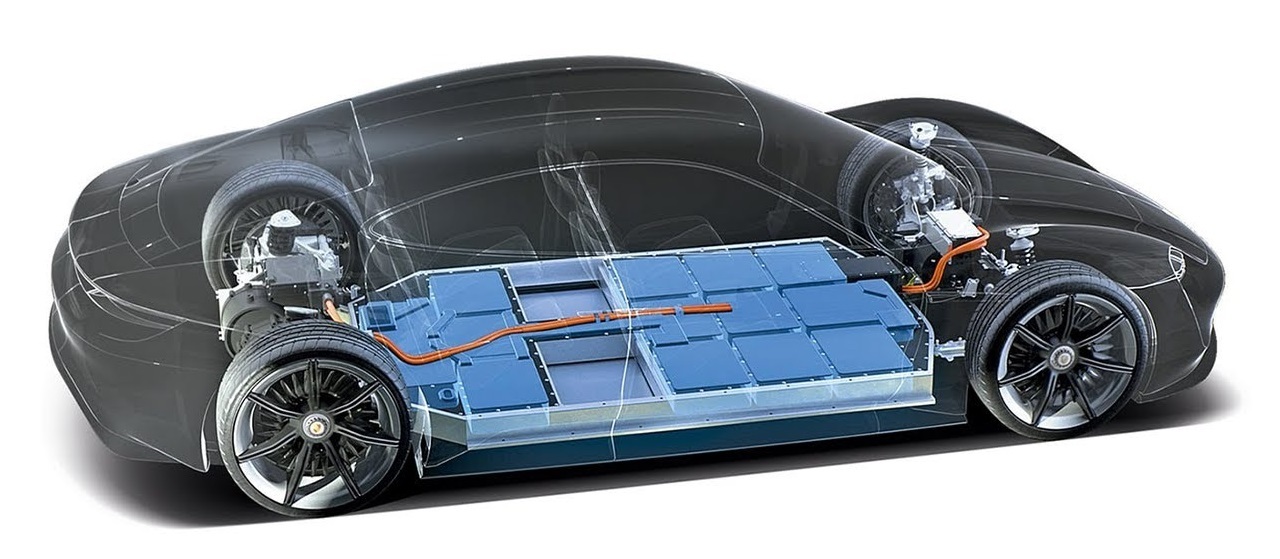
\includegraphics[width=0.9\textwidth]{images/porsche_taycan}
    \caption[An electric car and its battery pack]{An electric car (Porsche Taycan) with its battery pack highlighted. Taken from \cite{porsche_taycan}}
    \label{fig:porsche_taycan}
\end{figure}

A \textbf{battery management system} (BMS) is another important component in the design of an EV \cite{bms}. A BMS is an embedded software system which performs many functions related to the management of a battery pack, such as protecting the battery from operating outside its safe operating area (preventing overcharging and overdischarging, overcurrents, overheating), monitoring its state, calculating and reporting secondary data (such as the remaining driving range), balancing the state of charge among the battery cells and actively managing the battery pack's thermal management system (if present). All these operations are possible because of sensors installed inside the battery pack, which monitor parameters such as terminal voltage, current flow, internal temperature, state of charge and state of health (sec. \ref{sec:soh}) at the cell level. The BMS continuously monitors the sensors' measurements through a communication data bus, commonly known as Controller Area Network (CAN) bus. Moreover, these measurements can be communicated outside the vehicle through an interface called On-Board Diagnostics (OBD) port.

\section{Li-ion battery cell}
\label{sec:li-ion}
EV battery packs are hierarchically structured into three levels: cell, module
and pack \cite{li-ion_battery_properties}.
As visualized schematically in fig. \ref{fig:cell2module2battery}, multiple battery cells are first connected together in series and parallel to form a battery module, and then a certain number of modules are assembled to form a battery pack. This design has the aim of achieving a sufficiently high terminal voltage while adding up the capacity of each individual cell.

\begin{figure}[hbt!]
    \centering
    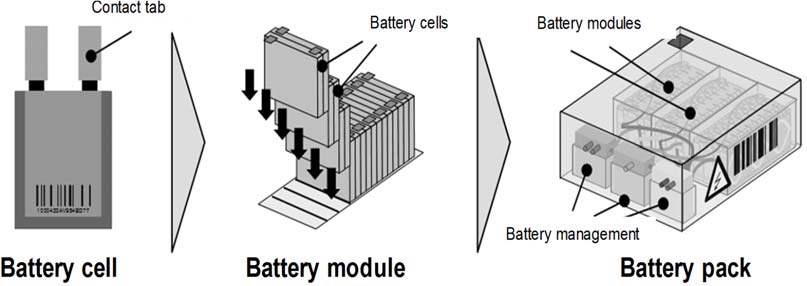
\includegraphics[width=0.8\textwidth]{images/cell2module2battery}
    \caption[From battery cells to a battery pack]{From battery cells to a battery pack. Taken from \cite{cell2module2battery}}
    \label{fig:cell2module2battery}
\end{figure}

Battery cells come in different formats (pouch, cylindrical, prismatic) and chemistries (choice of the anode and cathode materials and electrolyte), which together determine the energy density and efficiency, terminal voltage, safety characteristics, costs, and -- ultimately -- performances. They are typically named according to their cathode materials: for example, lithium-ion battery cells are characterized by lithium-based cathode materials such as lithium cobalt oxide (LiCoO2), lithium iron phosphate (LiFePO4), lithium nickel manganese cobalt oxides (LiNi\textsubscript{x}Mn\textsubscript{y}Co\textsubscript{z}O2, or NMC-xyz for short) and so on \cite{li-ion_chemistries}. Graphite is commonly used as anode material \cite{anode_material}. Cathode and anode are separated by a layer of electrolyte material, which is typically a polymer gel containing lithium salts\footnote{It is worth mentioning that recent advances in battery technology involve using a solid as the electrolyte material, with ceramics being the most promising \cite{solid_electrolyte}. Increased energy density, less need of thermal cooling and improved safety are among the many benefits of using a solid electrolyte.}. The electrolyte has two functions: it prevents the electrical contact between the two electrodes and, at the same time, it allows the diffusion of lithium ions (Li\textsuperscript{+}) from cathode to anode and vice versa.

When a battery is being discharged, Li\textsuperscript{+} ions are shuttled from
the anode to the cathode, forcing electrons to flow around an outside circuit and thus allowing the conversion of chemical energy
into electrical energy (fig. \ref{fig:li-ion_cell}). On the contrary, charging a battery rips Li\textsuperscript{+} ions out of cathode's oxide crystals and pulls them back to the graphite-based anode where they are stored \cite{nature_li-ion}.

\begin{figure}[hbt!]
    \centering
    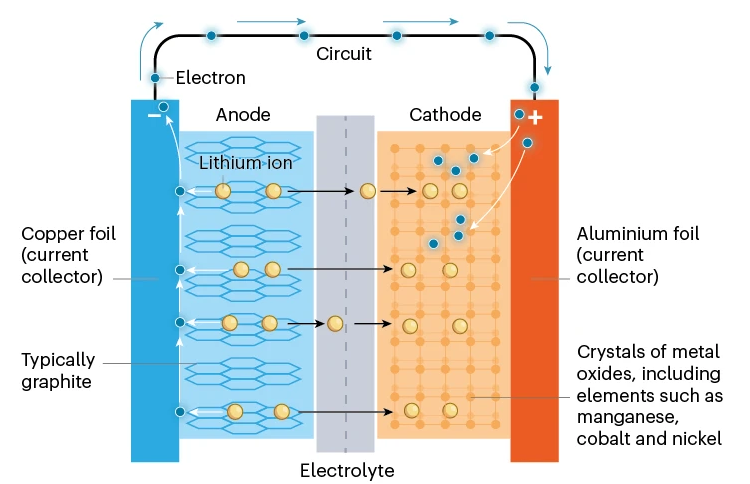
\includegraphics[width=0.8\textwidth]{images/li-ion_cell}
    \caption[Discharging a Li-ion battery cell]{Discharging a Li-ion battery cell. Taken from \cite{nature_li-ion}}
    \label{fig:li-ion_cell}
\end{figure}

\subsection{Battery cell aging and SOH}
\label{sec:soh}
Battery cells are characterized by many parameters describing their electrochemical state and dynamics. The \textbf{capacity} $C$ of a battery is defined as the total amount of charge it can deliver and is commonly measured in ampere-hours [Ah]. Manufacturers usually declare a nominal (or rated) capacity $C_{nominal}$, i.e. the capacity of the battery when it is fresh out of the factory. For instance, a battery rated at 60 Ah can theoretically deliver a current of 5 A for 12 hours. The more electrode material is contained in the cell, the greater is its capacity. Nonetheless, the open-circuit voltage of a battery cell depends solely on its chemistry, regardless of its capacity \cite{battery_glossary}. The ratio between the amount of charge $Q_{available}$ that can be extracted from the battery at a given point in time and the actual capacity $C_{actual}$ is called \textbf{state of charge}:
\begin{equation}
\label{eq:soc}
    SOC = \frac{Q_{available}}{C_{actual}}
\end{equation}

Actually, multiple external factors determine the effective battery capacity $C_{actual}$ at any given moment. Therefore, capacity is typically defined up to a nominal set of operating conditions (or \textbf{nominal conditions}, for short), namely: external temperature equal to room temperature ($\approx 20$ °C) and fixed discharge current magnitude. In fact, capacity tends to increase with high temperatures \cite{C_depends_on_T} and low discharge currents (a phenomenon called Peukert's law \cite{peukert}).

When dealing with a current flowing through a battery, we can also express its magnitude in terms of \textbf{C-rate}. It is defined as the magnitude of the current through the battery divided by the theoretical current draw under which the battery would deliver its capacity in one hour \cite{c-rate}. For instance, when referring to a battery with a capacity of 60 Ah, a current with C-rate 0.5 (or 0.5C current, for short) is a 30 A current.

Li-ion battery cells, like all batteries, are subject to degradation phenomena with time and usage, due to a variety of chemical and mechanical changes to the electrodes. These phenomena gradually lead to a decrease in capacity (a phenomenon called \textbf{capacity fading}) and an increase in internal resistance \cite{capacity_fading}. Other than normal usage in safe operating conditions, common causes of degradation include: shelving a full-charged battery for a long time, overcharging and overdischarging, storage or usage in very hot or very cold environments, high charge/discharge currents, discharging at high deltas of state of charge (depth of discharge, or DOD(\%) for short). There exist a large number of degradation mechanisms\footnote{This list is by no means exhaustive: an in-depth discussion of degradation mechanisms for Li-ion battery cells can be found in \cite{capacity_fading}.}, such as:
\begin{itemize}
    \item thickening of the Solid Electrolyte Interface (SEI), a passivation layer formed on the surface of LIBs' anode material produced by electrolyte decomposition, in which Li\textsuperscript{+} ions get irreversibly trapped (i.e. loss of lithium inventory)
    \item lithium plating, i.e. the deposition of lithium around the anode during charging
    \item loss of cathode and anode material due to its dissolution, cracking, exfoliation, detachment or volume change during usage
    \item corrosion and structural degradation of battery cell components, such as its current collectors.
\end{itemize}

Battery aging can be measured in a variety of ways. The most common way of quantifying the capacity loss of a battery is the \textbf{state of health} (SOH), defined as the ratio of the actual capacity of the battery to its nominal capacity:
\begin{equation}
\label{eq:soh}
SOH = \frac{C_{actual}}{C_{nominal}}
\end{equation}

Another way of expressing the age of a battery is the number of \textbf{equivalent full cycles} (EFC). An EFC is defined as a virtual cycle of charge and discharge of a battery at a specified DOD \cite{efc}. The number of EFCs can be estimated as
\begin{equation}
\label{eq:efc}
EFC = \int \frac{|I|}{2 \cdot DOD \cdot C_{nominal}} \, dt
\end{equation}
where $I$ is the current flowing through the battery. It is easy to observe that the SOH of a battery decreases as the number of EFCs increases; however, there is no general mathematical relationship between the SOH and the number of EFC, as the latter ignores operating conditions such as temperature and C-rate (as opposed to SOH), but also because SOH happens to not decrease uniformly over the lifespan of the battery \cite{efc,efc2}. For instance, at $T=25$ °C and a fixed 0.5C charging and discharging current a battery might undergo 3000 EFC at 100\% DOD before reaching a SOH of 80\%, while at $T=45$ °C and 2C current the same battery might undergo 1200 EFC before reaching 80\% SOH.

\subsection{From cell SOH to pack SOH}
\label{sec:cell_soh2pack_soh}
The cells inside a battery pack are subject to uneven degradation over time, due to their asymmetrical placement inside the pack, uneven temperature distribution, different inter-cell contact resistances and possible subtle differences in their manufacturing quality \cite{uneven_soh}. As a result, each individual cell is characterized by a different capacity and internal resistance. This in turn causes current to flow unevenly among the cells, worsening the imbalance of cell degradation rates. To break this vicious cycle, the BMS tries to balance temperatures and currents inside a battery pack according to the estimated SOH of each cell \cite{bms_balancing1,bms_balancing2}. Due to cell capacity imbalance and the complexity of the BMS, estimating the SOH at the battery pack level in real time is not an easy task.

In the context of EVs, a battery pack is said to be at its \textbf{end of life} (EOL) when its state of health reaches 80\% \cite{eol_def}. This threshold is commonly adopted since below 80\% of its SOH a Li-ion battery pack incurs in a faster, typically more-than-linear degradation \cite{soh_after_eol}.

Monitoring SOH is a critical task, since the EOL of a battery pack typically marks the time when it has to be retired. SOH estimation can be performed in a laboratory setting, but in recent years researchers devoted their efforts to designing real-time and on-board procedures to allow for an easier and cheaper alternative for estimating SOH, as discussed in sec. \ref{sec:aviloo} and chap. \ref{sec:state_of_the_art}.

\section{Proprietary SOH estimation procedures}
\label{sec:aviloo}
Nowadays, a few private EV fleet management companies developed reliable manufacturer-independent, on-board diagnostic procedures for EV battery packs. Typically, they provide such battery tests to customers wishing to assess the degradation of a battery pack before buying or selling an EV.

Such SOH estimation procedures typically consist in connecting a monitoring device to the OBD port of the car and then driving the fully charged vehicle until the SOC drops below 10\%. Meanwhile, the monitoring device continuously collects relevant operating data, which consists of measurements such as voltage, internal and external temperature, current, SOC, power consumption and so on, sampled with a relatively high frequency and possibly at the cell, module and pack level simultaneously. Finally, this data is used as the input of a proprietary SOH prediction algorithm, which provides the customer with a reliable estimate of the SOH of their EV's battery pack.

Some of these companies retain the collected EV field data. This data is invaluable as it can be used for further analyses on the monitored battery, but can also be exploited for research purposes. Indeed, such data is extremely useful in designing data-driven methods to predict the SOH of a battery pack, as discussed throughout this thesis.

%The field data collected during each bcheck can be viewed on a portal called AVILOO Battery Cloud, and consists of measurements such as voltage, internal and external temperature, current, SOC, power consumption and so on, sampled with a relatively high frequency and possibly at the cell, module and pack level simultaneously. EV monitoring data is extremely useful in designing data-driven methods to predict the SOH of a battery pack, as discussed throughout this thesis.


%AVILOO GmbH is an Austrian company born in 2017 with the mission of developing the first manufacturer-independent diagnostic procedure for EV battery packs. According to their website\footnote{ \url{https://aviloo.com/}\label{note:aviloo_website}}, they designed a reliable, on-board SOH estimation procedure with a claimed maximum estimation error of $\pm 1.5\%$. They provide their test to customers typically wishing to assess the degradation of a battery pack before buying or selling an EV.

%AVILOO Battery Test, also called \textbf{bcheck} (short for "battery check"), consists in connecting a monitoring device to the OBD port of the car, and then driving the fully charged vehicle until the SOC drops below 10\%. Meanwhile, the monitoring device continuously collects relevant data and sends it to AVILOO's servers. Then, this data is used as the input of AVILOO's SOH estimation algorithm. The customer finally receives a detailed certificate (fig. \ref{fig:aviloo_certificate}) reporting the estimated SOH value and other valuable information about the tested battery pack.

%\begin{figure}[hbt!]
%    \centering
%    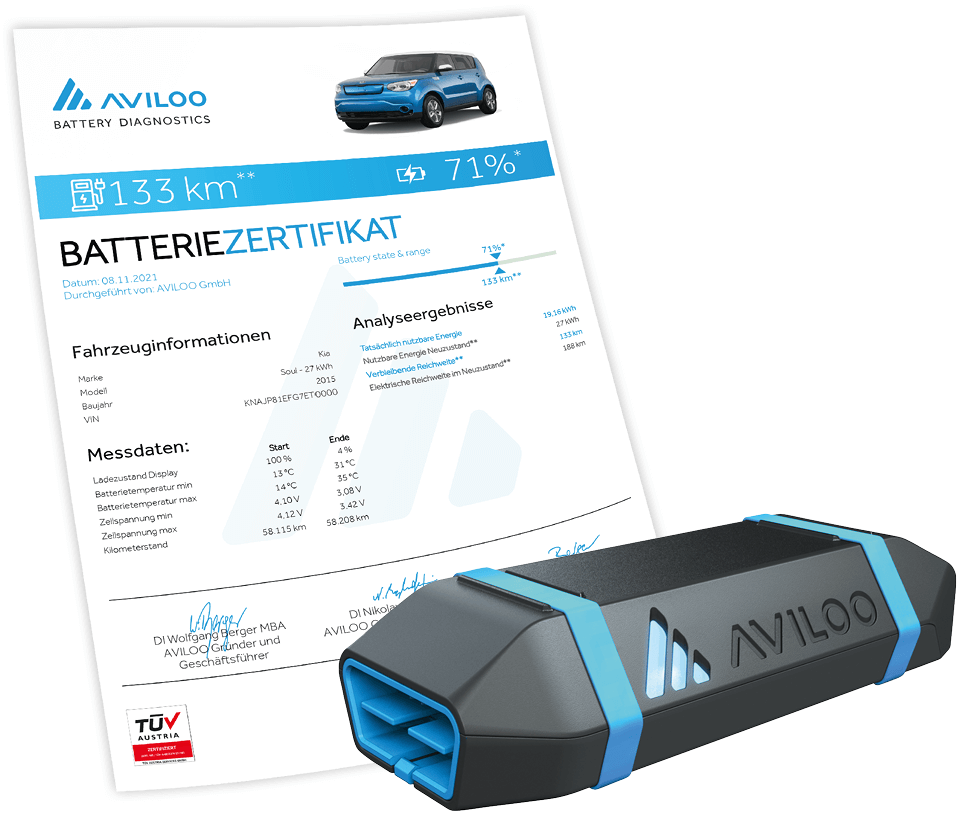
\includegraphics[width=0.9\textwidth]{images/aviloo_certificate.png}
%    \caption[AVILOO's battery test certificate and monitoring device]{AVILOO's battery test certificate and monitoring device. Taken from AVILOO's official website\footref{note:aviloo_website}.}
%    \label{fig:aviloo_certificate}
%\end{figure}

%The field data collected during each bcheck can be viewed on a portal called AVILOO Battery Cloud, and consists of measurements such as voltage, internal and external temperature, current, SOC, power consumption and so on, sampled with a relatively high frequency and possibly at the cell, module and pack level simultaneously. EV monitoring data is extremely useful in designing data-driven methods to predict the SOH of a battery pack, as discussed throughout this thesis.

% state of the art
\chapter{State of the art}
\label{sec:state_of_the_art}
In recent years, research on battery SOH estimation -- especially of Li-ion battery cells \cite{survey1} -- has been extensive and very diverse. In this chapter, a literature review of the existent SOH estimation methods is conducted.

\section{SOH estimation methodologies}
\label{soh_est_methods}
SOH estimation methods for Li-ion batteries mainly fall into three categories \cite{survey1}: direct measurement-based methods, model-based methods, data-driven methods. This taxonomy can be further expanded by observing that some of these methods can be (or are meant to be) used in real-time with sensor data recorded while driving or charging an EV (online methods), whereas others can only be applied away from usual EV operations (offline methods) \cite{survey2}.

\subsection{Direct measurement-based methods}
\label{sec:dmb_methods}
Direct measurement-based (DMB) methods compute relevant quantities directly from experimental battery data and use them to estimate the SOH. Their main advantage is that they are relatively easy to implement and are generally computationally cheap.

Coulomb counting \cite{coulomb_counting} is arguably the simplest offline DMB method. It estimates the SOH by integrating a discharge current signal over time, from full charge (SOC = 100\%) to full discharge (SOC = 0\%) of the battery. This value, which is the present capacity $C_{actual}$ of the battery, is then divided by the nominal capacity of the battery $C_{nominal}$, thus following def. \ref{eq:soh} exactly. This method has the advantage of being extremely cheap to apply, but its usage is typically confined to laboratory settings since EVs are typically never charged and discharged completely due to security hazards (namely overcharging and overdischarging \cite{overcharging}).

Electrochemical Impedance Spectroscopy (EIS) \cite{eis2} is a DMB method for measuring a battery's internal impedance by imposing different galvanostatic or potentiostatic excitation frequencies. Internal impedance is frequently employed as an alternative SOH indicator of a battery, since it tends to increase as the battery ages\footnote{When evaluating a battery's SOH in terms of internal resistance increase, the EOL of the battery is conventionally set to a 200\% increase of the initial internal resistance \cite{r_eol_convention}} \cite{eis3, survey3}. Despite exhibiting remarkable performances in SOH estimation \cite{eis2}, this method is deemed infeasible for online applications as it is computationally costly and requires sophisticated equipment which cannot be easily embedded on an EV \cite{survey1, survey3}.

Incremental capacity analysis (ICA) and differential voltage analysis (DVA) \cite{ica_dva1} are DMB methods based on the analysis of the evolution of a battery's incremental capacity and differential voltage curves. These curves are in fact correlated with battery aging (as shown in fig. \ref{fig:dva_img}), and can therefore be used to estimate SOH \cite{ica_dva2}. This method is computationally cheap, but it is only effective under low charge/discharge C-rates, a condition which cannot be ensured in real-world EV applications \cite{ica_dva3}.
\begin{figure}[hbt!]
    \centering
    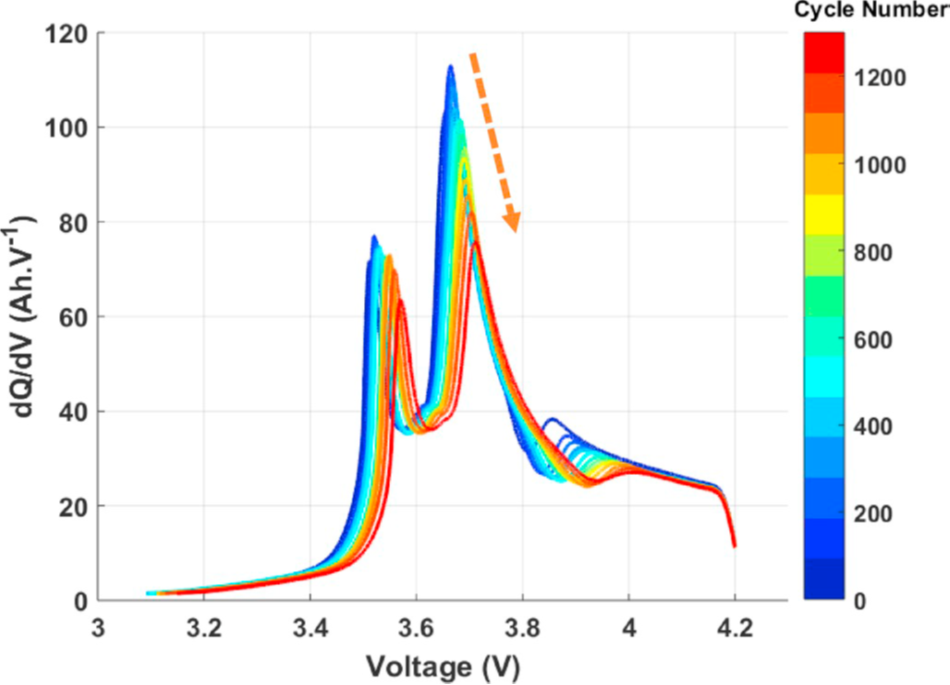
\includegraphics[width=0.6\textwidth]{images/dva_img}
    \caption[Incremental capacity curves at different cycles]{Incremental capacity curves for a high energy NMC/graphite cell under a charging current of 0.3C, after different charge/discharge cycles at ambient temperature. The peak intensity decreases and the peak location shifts to the right as more cycles are performed; these two quantities are therefore directly correlated with SOH. Taken from \cite{dva_img}}
    \label{fig:dva_img}
\end{figure}

\subsection{Model-based methods}
\label{sec:mb_methods}
Model-based (MB) methods build a mathematical model of a battery and estimate its parameters by fitting the model's dynamics to experimental battery data. The fitted parameters can then be used to estimate the SOH directly (as in DMB methods) or indirectly (as in DD methods). A variety of models exist, which describe the battery at different levels of physical abstraction.

Equivalent circuit models (ECM) \cite{survey1} are mathematical models of a battery based on electrical components such as resistors, capacitors and DC voltage sources, which describe the external characteristics of a battery \cite{ecm1}. A common ECM model is the $n$-th order RC model, which is schematized in fig. \ref{fig:rc_model}
\begin{figure}[hbt!]
    \centering
    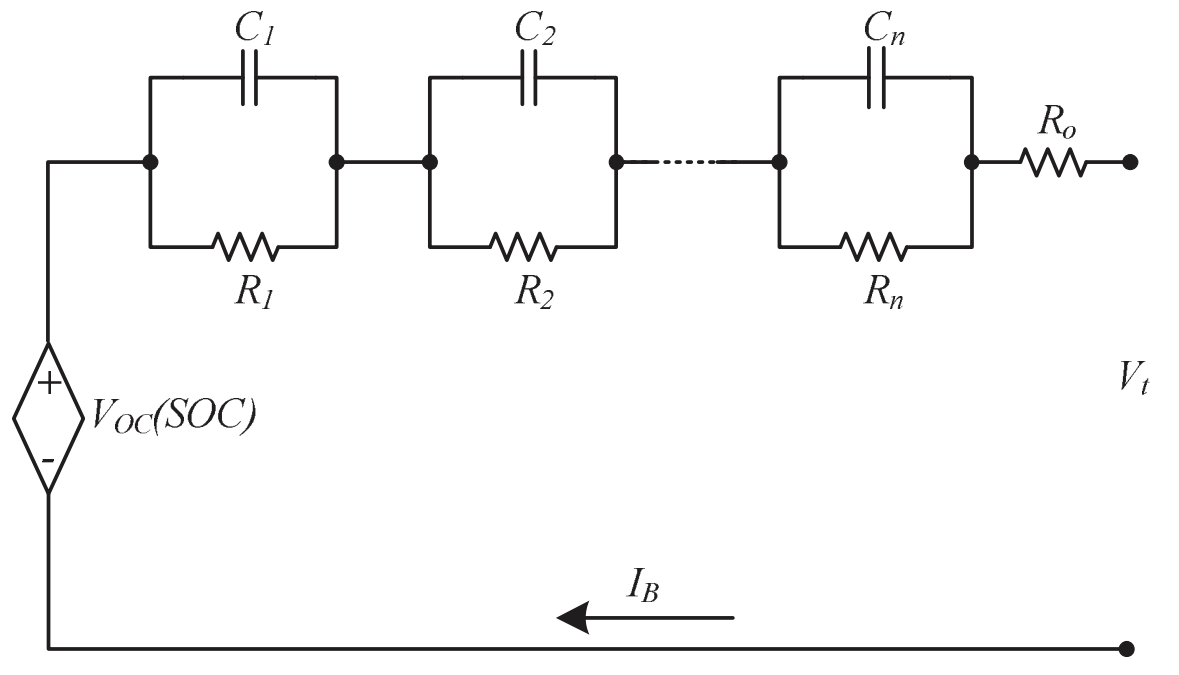
\includegraphics[width=0.6\textwidth]{images/rc_model}
    \caption[$n$-th order RC model of a battery]{$n$-th order RC model of a battery. Taken from \cite{ecm2}}
    \label{fig:rc_model}
\end{figure}
The components of this model are treated as look-up tables indexed by the battery's SOC, temperature and SOH. The parameters of an ECM model can be estimated through the available experimental data, by ensuring that the model's response to the experimental input current is compatible with the experimental output voltage. Increasing the order $n$ makes the model more expensive to fit, but increase its ability to better adapt to experimental data. Note that an ECM model is a mathematical abstraction of a battery: the electrical components which compose it do not have any physical meaning, and the complex physical and chemical dynamics inside a battery are basically ignored. Moreover, the computational cost of fitting a $n$-th order RC model significantly increases with $n$, and a larger amount of experimental data in different SOC, SOH and temperature conditions would be needed (which is often not publicly available) \cite{survey4}.

Similarly to ECM, empirical models (EM) \cite{survey2} are simple mathematical abstractions of a battery, which try to capture the non-linear relationship between SOH and degradation factors by means of a single function. Many possible degradation factors (such as temperature, age, SOC, \dots) and many possible functional forms (linear, exponential, logarithmic, \dots) can be chosen. However, just like ECM, EM need an extensive amount of data in different experimental conditions to be fitted accurately; moreover, the choice of the functional form of the model and the degradation factors to consider are highly dependent on the particular battery chemistry and may lead to overfitting the particular experimental data available.

The electrochemical model (EChM) \cite{survey1} tries to explicitly capture the complex physical and chemical phenomena which happen inside a battery and which cause capacity fading over time. The key assumption of this method is that the impedance spectrum of the battery is strongly related to the SOH. In practice, these physics-based electrochemical models generally achieve poor performances in the task of predicting the SOH of a battery, since a lot of physical and chemical properties must be identified and included in the model to accurately capture the dynamical behavior of a real battery \cite{survey2}. A high expertise of the battery cell architecture and chemistry is needed to design such models.

\subsection{Data-driven methods}
\label{sec:dd_methods}
Data-driven (DD) methods are a family of SOH approaches which leverage on large-scale datasets of experimental battery aging data, and whose performances are often dependent on the size and quality of such datasets \cite{survey5}. DD methods are gaining increasing interest due to their extreme flexibility and variety. Many DD methods have an additional advantage of being domain-agnostic, i.e. they do not require domain expertise in the fields of electronics and chemistry \cite{survey4}, as they automatically learn the relationship between experimental data and SOH.

DD methods based on machine learning and deep learning are becoming the most prominent approaches to SOH estimation \cite{survey2,survey3,survey4,survey5,tesi_filippo}. Different feature extraction techniques and different regression models are explored widely in literature \cite{survey1}. Usually, these methods require a relatively long offline training phase, in which EV monitoring data measured by the BMS is preprocessed and used for training a machine learning model, but they are quite fast and accurate at prediction time. Due to these advantages, machine learning methods are particularly suited for real-time, on-board SOH estimation.

This family of methods share some similarities with direct measurement-based methods \cite{survey5}, as they both deal with experimental data recorded by sensors during battery's operating life. However, the key difference is that DM methods exploit recorded experimental data to compute specific hand-crafted features and use them to estimate the SOH directly, whereas DD methods automatically learn relevant features from raw data which are then used to train machine learning models, often without the need of a domain expert. Nonetheless, there can be a bit of overlap between the two families; for instance, in a previous thesis work \cite{tesi_filippo} hand-crafted features were identified and extracted from raw EV monitoring data and used to train deep learning models for SOH prediction, thus taking advantage of both DM and DD methods.


\section{Literature review}
\label{sec:literature_review}
In this thesis work, a novel real-time SOH estimation approach based on machine learning methodologies is designed. Due to the extreme interest shown by both academia and industry towards machine learning-based SOH estimation methods in recent years, the literature on the topic is incredibly vast. For our scopes, we specifically select those publications which share some similarities with our approach\footnote{This literature review was conducted on several bibliographic databases, namely: MDPI, Science Direct (Elsevier), Springer, Wiley Online Library, IEEE Xplore.}.

\smallskip

One common choice adopted by many researchers is to exploit experimental data acquired when charging \cite{soh_charging1,soh_charging2,soh_charging3,soh_charging4,soh_charging5} or discharging \cite{soh_discharging1,soh_charging3} a battery cell in constant-current (CC) or constant-voltage (CV) modes. This choice is perhaps motivated by the particular stability of electrical signals such as voltage, SOC, and current during these operation modes, which allows for simpler estimation approaches. However, CC-CV discharge of a battery pack is feasible only in a laboratory setting, as these operation modes do not represent the randomized current load imposed to an EV battery pack during driving \cite{discharge_unstable}; moreover, even when a battery pack is charged in CC-CV mode, its single cells are generally not charged in the same way, since the BMS is able to assign different currents to different cells, as discussed in sec. \ref{sec:cell_soh2pack_soh}. Many works leverage on datasets which more accurately resemble real load conditions of EV battery packs, such as NASA Randomised Battery Usage Dataset \cite{nasa_dataset,auto_extr_soh_4,filippo_boni_paper,nasa_dataset_used1,nasa_dataset_used2} and Oxford Battery Degradation Dataset \cite{oxford_dataset,oxford_dataset_used1,oxford_dataset_used2,oxford_dataset_used3}.
Raw experimental data acquired from sensors is typically not used directly; rather, the majority of the approaches found in literature extract relevant features which are assumed to be correlated with the SOH.

Roman et al. \cite{manual_extr_soh_13} proposed a manual feature extraction pipeline in which a total of 30 features are identified; recursive feature elimination based on random forests filters out the least relevant features for the SOH regression task and several regression models are trained on an augmented version of the resulting dataset. Among these models, random forest, deep neural network
ensemble, Bayesian ridge regression and Gaussian process regression are explored.

Many other traditional regression models have been applied to SOH prediction pipelines. Among these: support vector regression \cite{soh_svr}, linear regression models (Ridge, Lasso, Elastic net) \cite{soh_ridge} and several variations of feed-forward neural networks (FFNN) \cite{soh_nn1, soh_nn2, soh_nn3}.

Deep learning (DL) models are also widely explored. Chemali et al. \cite{auto_extr_soh_2} developed a SOH estimation method based on a convolutional neural network (CNN), which is given raw charging data (voltage, current and temperature over time) as input. The advantage of this methodology consists in getting rid of the manual feature engineering, as a CNN automatically learns how to extract relevant features from raw data.

More complex DL methods have been adapted to the task of predicting the SOH of a battery cell, namely Recurrent Neural Networks (RNN) \cite{soh_rnn}, Long Short-Term Memory (LSTM) \cite{soh_lstm}, Gated Recurrent Units (GRU) \cite{soh_gru}, independent recurrent neural networks (IndRNN) \cite{soh_indrnn} and many more.

\smallskip

We highlight that all of these methods leverage on experimental data regarding single battery cells, mostly due to the unavailability of public datasets of EV battery packs' monitoring data. A further step needs to be taken in order to scale up from single battery cells to whole battery packs. Interestingly, Merkle et al. \cite{soh_digital_twin} introduced a digital battery twin for a 2014 Volkswagen e-Golf, setting up a data pipeline to predict the battery pack's SOC and SOH in real time. They acquired a training dataset directly from the OBD interface during a real drive cycle; however, this dataset has not been made publicly available. Song et al. \cite{manual_extr_soh_7} trained their SOH estimation methodology on a seemingly large public dataset of battery pack monitoring data collected by Shanghai Electric Vehicle Public Data Collecting, Monitoring and Research Center (SHEVDC). Despite their claim of being "the world's largest [public] platform for data collection and analysis of new energy vehicles", the Data Center requires researchers to apply for a membership in order to be granted access to the dataset\footnote{The application process seems unnecessarily long and rather obscure for a self-proclaimed "public" data center; for reference, it can be found on SHEVDC website: \url{http://en.cctp.org.cn/product/type/3849-8780-1.html}.}.

To make up for the lack of publicly available EV monitoring data, a possible solution is generating such data artificially \cite{li-ion_data_where}. This can be achieved in a variety of ways; one possible solution is exploiting an EV model implemented on a simulation software such as Simulink \cite{ev_simulink_model1,ev_simulink_model2,ev_simulink_model3,ev_simulink_model4,ev_simulink_model5,racing_lounge} to simulate realistic drive cycles and gather synthetic electrical and mechanical signals from simulations. This is the approach followed in this thesis work: an existing EV model \cite{racing_lounge} is adapted (sec. \ref{sec:model_parametrization}) and then used (sec. \ref{sec:ds_gen}) to generate a large dataset of voltage, current, temperature and SOC measurements. This dataset is then used to train a regression procedure for the SOH estimation (chap. \ref{sec:experiments}).

% methodology
\chapter{Methodology}
\label{sec:methodology}
In this chapter, an overview of the concepts, algorithms and machine learning models encountered throughout this thesis work is provided.

\section{Optimization problems}
\label{sec:opt_prob}
Everything in machine learning comes down to an optimization problem.

Optimization is the problem of finding one or more points that minimize or maximize a given objective function.

\begin{definition}[Optimization problem]
Let $J:A \subseteq \mathbb{R}^n \to \mathbb{R}$. The problem of finding a global minimizer $\mathbf{x^*} \in B \subseteq A$ of $J$ is an called optimization problem.
\end{definition}
$B$ is called the \textit{search space}. When $A=B$, the optimization problem is \textit{unconstrained}, whereas if $A \subset B$ it is \textit{constrained}; in constrained optimization problems typically $B$ is defined by a set of constraints, i.e. equalities and/or inequalities that points in $B$ have to satisfy. Points in $B$ are called \textit{feasible solutions}, whereas all the possible $\mathbf{x^*}$ (if existent) are called \textit{optimal solutions}.

There are a number of results which guarantee the existence and uniqueness of the optimal solution(s) of an optimization problem.

\begin{definition}[Convex set]
A set $C \subseteq \mathbb{R}^n$ is convex if $\forall \mathbf{x},\mathbf{y} \in C$ the segment joining $\mathbf{x}$ and $\mathbf{y}$ is contained in $C$:
\[
\alpha \mathbf{x} + (1-\alpha)\mathbf{y} \in C \qquad \forall \alpha \in (0,1)
\]
\end{definition}

\begin{definition}[Convex function]
Given a convex set $C \subset \mathbb{R}^n$, a function $f:C \to \mathbb{R}$ is convex if
\[
f(\alpha \mathbf{x}+(1-\alpha)\mathbf{y}) \leq \alpha f(\mathbf{x}) + (1-\alpha) f(\mathbf{y}) \qquad \forall \mathbf{x},\mathbf{y} \in C, \; \alpha \in (0,1)
\]
\end{definition}
If the inequality in the definition holds strictly, then the function is strictly convex.

\begin{theorem}
If $f$ is convex on $B$, local minimizers of $f$ in $B$ are also global minimizers. Moreover, if $f$ is also strictly convex on $B$, then there exist a unique global minimizer of $f$ in $B$.
\end{theorem}

An optimization problem is (strictly) convex if $J$ is a (strictly) convex function. In machine learning, the objective function $J$ is usually a continuous non-linear function, and it is commonly called \textit{cost function}.

Direct methods for solving non-linear optimization problems are often too impractical. Luckily, there exist a huge number of \textbf{iterative methods} for solving optimization problems, i.e. methods which construct a sequence $\mathbf{x}_0,\mathbf{x}_1,\dots$ which are asymptotically likely to converge to the optimal solution. Three of them are discussed hereafter: gradient descent (sec. \ref{sec:gradient_descent}), stochastic gradient descent (sec. \ref{sec:sgd}), Nelder-Mead method (sec. \ref{sec:nelder_mead}).



\subsection{Gradient descent}
\label{sec:gradient_descent}
\textbf{Gradient descent} \cite{gd} is an iterative method in which the iterates $\mathbf{x}_k$ are obtained by moving along the local direction of steepest descent, i.e. $-\nabla J(\mathbf{x}_k)$:
\begin{equation}
\mathbf{x}_{k+1} = \mathbf{x}_k - \eta \nabla J(\mathbf{x}_k)
\end{equation}
Basically, at each step the gradient descent algorithm locally builds a first-order approximation of $J$ at $\mathbf{x}_k$, and then moves along the local direction of most rapid decrease of $J$ (which is minus the gradient of $J$ at $\mathbf{x}_k$) until a stopping criterion is met (e.g. threshold on $\norm{J(\mathbf{x}_{k+1}) - J(\mathbf{x}_k)}$ reached and/or maximum number of iterations reached; both are user-specified hyperparameters).

In machine learning, the step-length $\eta \in \mathbb{R}$ is commonly known as \textit{learning rate}. It is a user-defined hyperparameter which must be chosen carefully: a learning rate which is too high may make the method fail to converge, whereas a learning rate which is too low may slow down convergence. This is exemplified in fig. \ref{fig:lr_choice}.

\begin{figure}[hbt!]
    \centering
    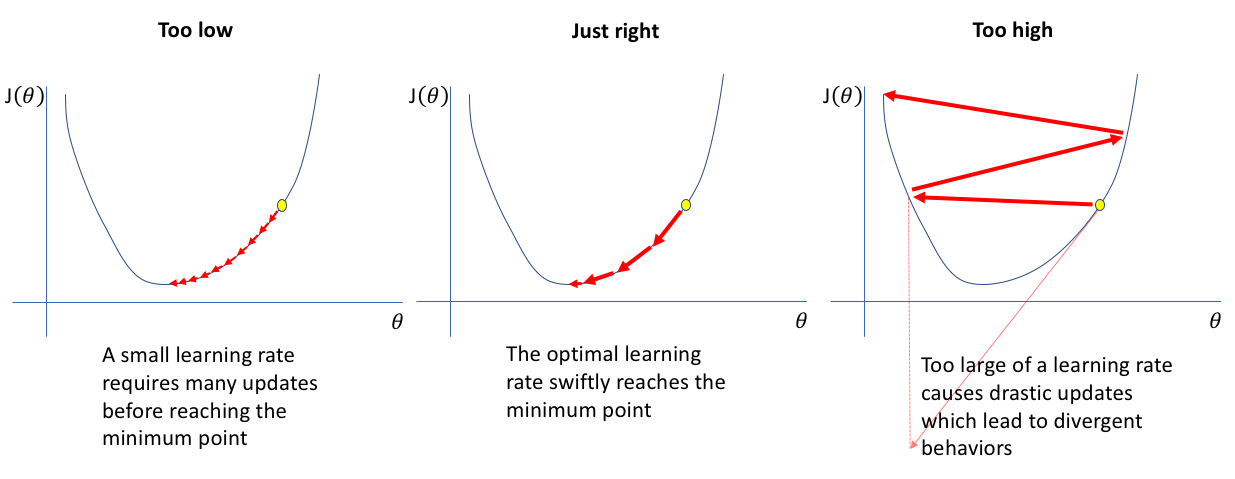
\includegraphics[width=\textwidth]{images/lr_choice}
    \caption[Choice of the learning rate of gradient descent]{The importance of choosing an appropriate learning rate for the gradient descent algorithm. Taken from \cite{lr_choice}}
    \label{fig:lr_choice}
\end{figure}

Typically, when the method is approaching the minimum of the function that is being optimized, we may want to decrease the learning rate to allow more fine-grained updates. There exists a huge variety of rules and schedules for the update of the learning rate \cite{lr_schedules}. Among them:
\begin{itemize}
    \item Reduce $\eta$ by a factor $\xi \in (0,1)$ when $\norm{J(\mathbf{x}_{k+1}) - J(\mathbf{x}_k)}$ is below a specified threshold $T$ for at least $P$ iterations. $\xi$ (learning rate decay factor), $T$ (tolerance) and $P$ (patience) are all user-specified hyperparameters (and they can be scheduled as well!). Typically implemented when training neural networks (sec. \ref{sec:neural_network}).
    \item Reduce $\eta$ at each step by a factor $g(k)$ where $g$ is a decreasing function of $k$ (e.g. $g(k) = \frac{1}{k^p}$, with $p>0$ hyperparameter). $g$ is a user-specified hyperparameter. Used by default in scikit-learn when training ridge regression (sec. \ref{sec:ridge}) via SGD.
\end{itemize}

Also the choice of the initial point $\mathbf{x}_0$ is of particular importance: choosing it to be near the effective minimum of the function may speed up the convergence of the method. However, quite obviously, this information is almost never available, and we must resort to random initialization.

\smallskip

Since non-linear functions are not convex in general, they may have many local minima, as shown in fig. \ref{fig:nonconvex_function}.
\begin{figure}[hbt!]
    \centering
    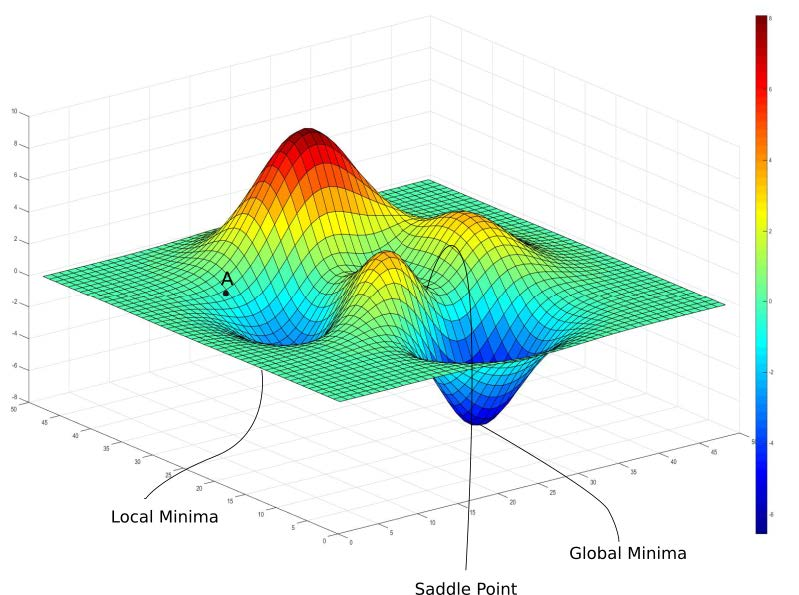
\includegraphics[width=0.9\textwidth]{images/nonconvex_function}
    \caption[A non-convex bivariate function]{A non-convex bivariate function. Taken from \cite{nonconvex_function_img}}
    \label{fig:nonconvex_function}
\end{figure}

A common problem that arises when using gradient descent on a non-linear objective function is that iterates may converge to a local minimum of $J$, especially when the initial point $\mathbf{x}_0$ is already closer to a local minimum than a global one. This issue can be avoided by resorting to other iterative methods which are more robust to the initialization of the starting point, e.g. stochastic gradient descent (sec. \ref{sec:sgd}).

\subsection{Stochastic gradient descent}
\label{sec:sgd}
In machine learning, the cost function $J$ to be minimized is often built upon a dataset $\mathcal{D} = \{(\mathbf{x}_1,y_1),\dots,(\mathbf{x}_N,y_N)\}$ and has the form
\begin{equation}
J(\bm{\theta};\mathcal{D}) = \frac{1}{N} \sum_{i=1}^N \ell(\bm{\theta};\mathbf{x}_i,y_i) + R(\bm{\theta})
\end{equation}
where $R$ is a regularization term and the function $\ell$ in each summand is commonly known as \textit{loss function}, and is parametrized only by a single data point $(\mathbf{x}_i,y_i)$. For instance, the mean squared error (MSE) is a cost function which uses the squared difference between the predicted value $\hat{y}=f(\mathbf{x};\bm{\theta})$ and the real value $y$ as loss function: $\ell(\bm{\theta}; \mathbf{x}, y) = (f(\mathbf{x};\bm{\theta}) - y_i)^2$.

\textbf{Stochastic gradient descent} (SGD) \cite{sgd} is a variant of the gradient descent method in which at each iteration the cost function to be minimized is constructed only on a random subset $\mathcal{B}$ of $\mathcal{D}$ (called \textit{minibatch}). This constitutes a stochastic approximation of the loss function. The size of each minibatch is an hyperparameter; a higher batch size ensures a better approximation of $J$ (which therefore exhibits approximately the same minima of $J$), but determines a slower convergence due to the additional computational cost of computing the gradient. A \textit{training epoch} (or simply \textit{epoch}) refers to one sweep through the entire training set; therefore, a training epoch consists of $\ceil{|\mathcal{D}|/|\mathcal{B}|}$ iterations of the method\footnote{There are $|\mathcal{D}|$ mod $|\mathcal{B}|$ samples left out from any minibatch; a typical choice is to ignore them during the current epoch}. At each epoch, the samples of each minibatch are randomly sampled from $\mathcal{D}$ without replacement. Iterations halt at the end of a user-specified number of epochs, or when other stopping criteria are met (e.g. the learning rate goes below a user-defined threshold).

SGD has several benefits over simple gradient descent:
\begin{itemize}
    \item SGD is more robust to the initialization of $\mathbf{x}_0$ than gradient descent, since the varying cost function at each iteration ensures that the method is less likely to get stuck in local minima.
    \item SGD typically requires more iterations than gradient descent to converge to a minimum, but a single iteration of SGD is computationally cheaper than those of gradient descent. Overall, SGD is faster than gradient descent in terms of computational time, especially when $\mathcal{D}$ is large.
    \item SGD can handle very large training sets, because during each iteration only a minibatch of data must be stored in memory.
\end{itemize}

Gradient descent and SGD are visually compared in fig. \ref{fig:gd_vs_sgd}

\begin{figure}[htb!]
\centering
\begin{subfigure}[t]{0.475\textwidth}
    \centering
    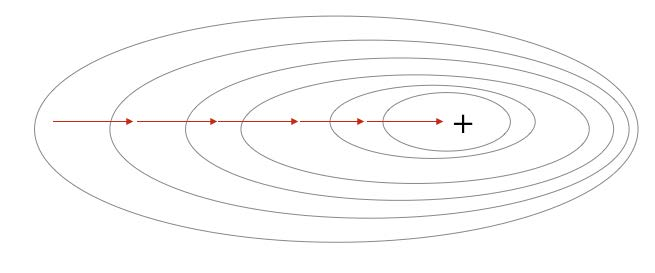
\includegraphics[width=\textwidth]{images/gd}
    \caption{}
\end{subfigure}
\hfill
\begin{subfigure}[t]{0.475\textwidth}
    \centering
    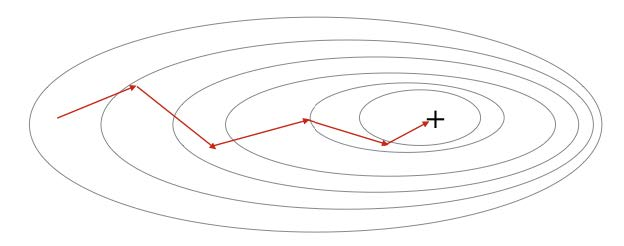
\includegraphics[width=\textwidth]{images/sgd}
    \caption{}
\end{subfigure}
\caption[Minimizing a function through GD and SGD]{Minimizing a bivariate function through (a) gradient descent (b) stochastic gradient descent. Taken from \cite{gd_images}}
\label{fig:gd_vs_sgd}
\end{figure}

\subsubsection{SGD with momentum}
\textbf{SGD with momentum} (SGD-M) \cite{sgd-m} is a variant of the standard SGD method. It changes the usual iterative update of gradient descent and SGD to
\begin{align}
\mathbf{v}_{k+1} &= -\eta \nabla J(\mathbf{x}_k) + \mu \mathbf{v}_k \\
\bm{\theta}_{k+1} &= \bm{\theta}_k + \mathbf{v}_{k+1}
\end{align}
with $\mathbf{v}_0=0$ and where factor $\mu \in (0,1)$ is an hyperparameter. The term $\mathbf{v}_k$ is called \textit{momentum}. This "perturbation" to the direction along which to perform the update has the effect of preserving some information about the previously chosen directions\footnote{The term "momentum" has a meaning similar to that of momentum in physics: when an object is moving it is said to possess momentum, i.e. the product between its mass and (vectorial) velocity; if a force is applied to the object in a generic direction, the object gains momentum in that direction, losing the momentum it already possessed only due to friction. Similarly, in an update of the SGD with momentum we can view $-\nabla J(\bm{\theta}_k)$ as a force which gives the iterates "momentum" along its direction, and this momentum is preserved "by inertia", making the descent path more stable in comparison to that of SGD.} and performing an update also in those directions, ultimately making the descent path less noisy than standard SGD. A visual interpretation of SGD-M is reported in fig. \ref{fig:sgd-m}.

\begin{figure}[hbt!]
    \centering
    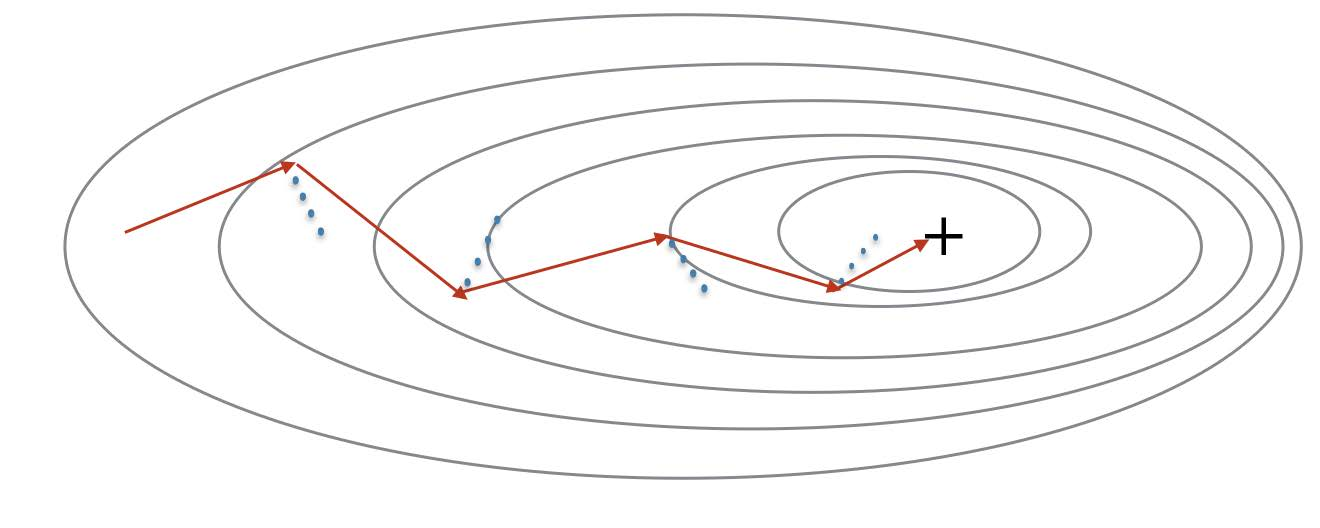
\includegraphics[width=0.475\textwidth]{images/sgd-m}
    \caption[Minimizing a function through SGD-M]{Minimizing a bivariate function through stochastic gradient descent with momentum. Taken from \cite{gd_images}}
    \label{fig:sgd-m}
\end{figure}



\subsection{Nelder-Mead method}
\label{sec:nelder_mead}
\textbf{Nelder-Mead method} \cite{nelder_mead} is a derivative-free iterative method for solving optimization problems. It is useful when we know how to compute the value of the objective function $J$ but not how to evaluate its gradient (or when the gradient is too computationally expensive to compute).

Nelder-Mead method is based on the concept of \textit{simplex}.
\begin{definition}[Simplex]
A $n$-dimensional simplex $\mathcal{S}$ is the convex hull of $n+1$ points $\mathbf{x}_i \in \mathbb{R}^n$, i.e.
\[
\mathcal{S} = \left\{\mathbf{y}\in\mathbb{R}^n \; \middle| \; y=\sum_{i=1}^{n+1} \lambda_i \mathbf{x}_i, \; \lambda_i \geq 0, \; \sum_{i=1}^{n+1}\lambda_i = 1\right\}
\]
The points $\mathbf{x}_i$ ($i=1,\dots,n+1$) are called vertices of $\mathcal{S}$.
\end{definition}
$\mathcal{S}$ is said to be non-singular if $\mathbf{x}_2 - \mathbf{x}_1$, \dots, $\mathbf{x}_{n+1} - \mathbf{x}_1$ are linearly independent. For instance, a line segment is a non-singular simplex in $\mathbb{R}^1$, a triangle in $\mathbb{R}^2$, a tetrahedron in $\mathbb{R}^3$ and so on.

The basic idea of Nelder-Mead method is to start with a given simplex $\mathcal{S}_0$ and modify it at each iteration ($\mathcal{S}_1, \mathcal{S}_2, \dots$) until a suitable simplex is found which provides a good approximation of the optimal solution of the problem.

A generic iteration $k$ of the method is taken from \cite{nelder_mead_implementation} and reported hereafter. Let $\mathcal{S}_k$ be a given non-singular simplex and let $\mathbf{x}_1^{(k)}, \dots, \mathbf{x}_{n+1}^{(k)}$ be its vertices. Assume that the vertices are ordered in such a way that $f(\mathbf{x}_1^{(k)}) \leq \dots \leq f(\mathbf{x}_{n+1}^{(k)})$ (so $\mathbf{x}_1$ is the "best" point of the simplex and $\mathbf{x}_{n+1}^{(k)}$ is the "worst"). We perform the following steps sequentially:

\begin{enumerate}
    \item \textbf{Ordering phase}\\
    Evaluate $f$ at the $n+1$ vertices of $\mathcal{S}_k$ and order the values $f(\mathbf{x}_i^{(k)})$ in increasing order ($f(\mathbf{x}_1^{(k)}) \leq \dots \leq f(\mathbf{x}_{n+1}^{(k)})$), and correspondingly order the vertices of $\mathcal{S}_k$.
    \item \textbf{Reflection phase}\\
    Let $\mathbf{\overline{x}}^{(k)} = \frac{1}{n}\sum_{i=1}^n \mathbf{x}_i^{(k)}$ be the barycenter of the $n$ best points and compute a reflection $\mathbf{x}_R^{(k)}$ of $\mathbf{x}_{n+1}^{(k)}$ w.r.t. $\overline{\mathbf{x}}^{(k)}$:
    \[
    \mathbf{x}_R^{(k)} = \overline{\mathbf{x}}^{(k)} + \rho (\overline{\mathbf{x}}^{(k)} - \mathbf{x}_{n+1}^{(k)})
    \]
    If $f(\mathbf{x}_1^{(k)}) \leq f(\mathbf{x}_R^{(k)}) \leq f(\mathbf{x}_n^{(k)})$, then we accept $\mathbf{x}_R^{(k)}$ as a new vertex of $\mathcal{S}_{k+1}$ in place of $\mathbf{x}_{n+1}^{(k)}$ and go back to step 1, else go to step 3.
    \item \textbf{Expansion phase}\\
    If $f(\mathbf{x}_R^{(k)}) < f(\mathbf{x}_1^{(k)})$ then compute an expansion $\mathbf{x}_E^{(k)}$ as
    \[
    \mathbf{x}_E^{(k)} = \overline{\mathbf{x}}^{(k)} + \chi (\mathbf{x}_R^{(k)} - \overline{\mathbf{x}}^{(k)})
    \]
    else go to step 4.
    If $f(\mathbf{x}_E^{(k)}) < f(\mathbf{x}_R^{(k)})$ then we accept $\mathbf{x}_E^{(k)}$ as a new vertex of $\mathcal{S}_{k+1}$ in place of $\mathbf{x}_{n+1}^{(k)}$ and go back to step 1. Otherwise accept $\mathbf{x}_R^{(k)}$ as a new vertex of $\mathcal{S}_{k+1}$ in place of $\mathbf{x}_{n+1}^{(k)}$ and go back to step 1.
    \item \textbf{Contraction phase}\\
    Compute a contraction $\mathbf{x}_C^{(k)}$ between $\overline{\mathbf{x}}^{(k)}$ and the best among $\mathbf{x}_R^{(k)}$ and $\mathbf{x}_{n+1}^{(k)}$ as
    \[
    \mathbf{x}_C^{(k)} =
    \begin{dcases}
        \overline{\mathbf{x}}^{(k)} - \gamma (\overline{\mathbf{x}}^{(k)} - \mathbf{x}_{n+1}^{(k)}) & \text{if } \mathbf{x}_{n+1}^{(k)} < \mathbf{x}_n^{(k)}\\
        \overline{\mathbf{x}}^{(k)} - \gamma (\overline{\mathbf{x}}^{(k)} - \mathbf{x}_R^{(k)}) & \text{otherwise}\\
    \end{dcases}
    \]
    If $f(\mathbf{x}_C^{(k)}) < f(\mathbf{x}_{n+1}^{(k)})$ then we accept $\mathbf{x}_C^{(k)}$ as a new vertex of $\mathcal{S}_{k+1}$ in place of $\mathbf{x}_{n+1}^{(k)}$ and go back to step 1. Else go to step 6.
    \item \textbf{Shrinking phase}\\
    Compute
    \[
    \mathbf{x}_i^{(k)} = \mathbf{x}_1^{(k)} + \sigma (\mathbf{x}_i^{(k)} - \mathbf{x}_1^{(k)}) \qquad \forall i=2,\dots,n+1
    \]
    and go back to step 1.
\end{enumerate}

A generic iteration of the Nelder-Mead method is visualized in fig. \ref{fig:nelder_mead}.

\begin{figure}[hbt!]
    \centering
    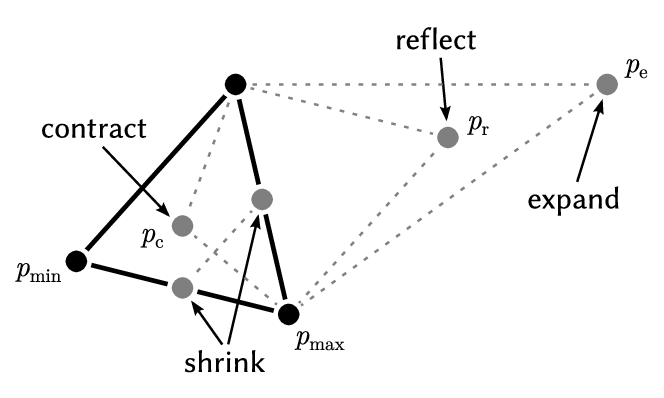
\includegraphics[width=0.6\textwidth]{images/nelder_mead}
    \caption[An iteration of the Nelder-Mead method]{An iteration of the Nelder-Mead method applied to a function $J:\mathbb{R}^2 \to \mathbb{R}$. Taken from \cite{wiki:nelder_mead}}
    \label{fig:nelder_mead}
\end{figure}

The method ends when a stopping criterion is met (e.g. maximum number of iterations reached or when $\norm{f(\mathbf{x}_{n+1}^{(k)}) - f(\mathbf{x}_{1}^{(k)})}$ is below a user-defined threshold). This method is based on the following 4 hyperparameters:
\begin{itemize}
    \item $\rho$: reflection parameter ($\rho>0$)
    \item $\chi$: expansion parameter ($\chi>1, \chi>\rho$)
    \item $\gamma$: contraction parameter ($0<\gamma<1$)
    \item $\sigma$: shrinking parameter ($0<\sigma<1$)
\end{itemize}
Typical choices are: $\rho=1$, $\chi=2$, $\gamma=1/2$, $\sigma=1/2$ \cite{nelder_mead_implementation}. 

The choice of the initial simplex $\mathcal{S}_0$ is also critical. In fact, an initial simplex that is too small can lead to a local search, and in this case the Nelder-Mead method can get more easily stuck.

Although there are no known convergence guarantees for Nelder-Mead method, it is nonetheless widely used because it is computationally cheap and does not require that $J$ is differentiable (continuity is enough).





\section{Time series}
\label{sec:time_series}
Monitoring a driving session of an EV means measuring and recording physical quantities such as vehicle speed, battery voltage, current, SOC and temperature over time. From a mathematical perspective, these discrete-time physical signals, along with the timestamps at which the measurements have been taken, can be treated as a multivariate time series.

\begin{definition}[Time series]
\label{def:ts}
A time series $S$ is an ordered collection of $T$ pairs of timestamps and tuples of $C$ measurements
\[
S=\{(t_1,\mathbf{s}_1),(t_2,\mathbf{s}_2),\dots,(t_T,\mathbf{s}_T)\}
\]
where $t_i \in \mathbb{R}^+$ and $\mathbf{s}_i \in \mathbb{R}^C$.
\end{definition}
It follows that a time series can be thought of as a $C\times T$ matrix.

The number of timestamps, $T$, is also called \textit{length} of the time series, and the number of measurements taken at each timestamp, $C$, is also known as the \textit{number of channels} (or \textit{dimensions}) of the time series; if $C=1$, the time series is \textit{univariate}, whereas if $C>1$ it is \textit{multivariate}. The ordered set of timestamps $t_1,\dots,t_T$ is called \textit{time base} of the time series.\footnote{Def. \ref{def:ts} doesn't take into account those multivariate time series for which each channel has a different time base. However, we can still use the above definition by fixing a "shared" time base (the ordered union of the $C$ different time bases) and opportunely adding \textit{null} values where measurements are not available.} If the time series has an unevenly spaced time base, it is called \textit{unevenly spaced} time series.

An example of a 4-channel multivariate time series (extracted from a real set of EV monitoring data, chap. \ref{sec:aviloo_ds}) is visualized in fig. \ref{fig:ts_example}.

\begin{figure}[hbt!]
    \centering
    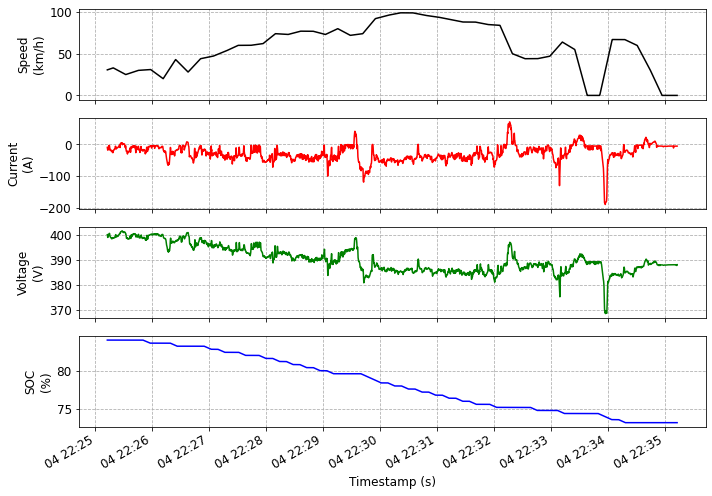
\includegraphics[width=\textwidth]{images/ts_example}
    \caption[A multivariate time series with 4 channels]{A multivariate time series with $C=4$ channels.}
    \label{fig:ts_example}
\end{figure}

Many time windows of monitoring data, along with the SOH value of the battery pack at the particular time the vehicle was driven, form a time series dataset.
\begin{definition}[Time series dataset]
\label{def:ts_ds}
A time series dataset $D$ is a collection of $N$ instances (or \textit{samples})
\[
D = \{(S_1,y_1), (S_2,y_2), \dots, (S_N,y_N)\}
\]
where $S_i$ is a time series and $y_i$ is a scalar value (called \textit{ground-truth label}, \textit{target variable}, \textit{response variable} or \textit{observation}).
\end{definition}
The collection of time series composing the dataset, ($S_1,\dots,S_N)$, can be thought of as a $N \times C \times T$ tensor.

\subsection{Time series extrinsic regression}
\label{sec:tser}
Time series datasets often show up in experimental settings. For this reason, in the past decade there has been an increasing interest in time series analysis research \cite{TSER}. Common tasks in time series analysis are:
\begin{itemize}
    \item Time series classification (TSC): the problem of assigning a label, taken from a finite discrete label set, to a time series
    \item Time series forecasting (TSF): the problem of predicting future values of a time series based on the past measurements; also known as time series regression (TSR)
    \item Time series extrinsic regression (TSER): the problem of assigning a scalar value to a time series
\end{itemize}

TSER is a generalization of both TSC and TSF. The difference between TSER and TSC is that the value to predict is discrete and categorical in TSC, and continuous in TSER; the difference between TSER and TSF is that in TSF the scalar value to predict is some future measurement of the time series, whereas in TSER this assumption is relaxed.

We may frame the problem of predicting the SOH of the battery pack of an EV as a TSER problem: we seek to find a mapping from a time series of driving session monitoring data (with channels such as voltage, current, SOC, temperature, etc.) to the SOH of the battery pack (a scalar in the range [0,100]). In the context of machine learning, such a mapping is also called a \textit{regression model}.

\subsection{Time series feature extraction}
In many experimental settings, the length of the recorded time series is too long in order to train a regression model directly on raw time series data: this is because each measurement is regarded as a feature, and many machine learning algorithms do not scale well with the number of features of a dataset \cite{ts_feat_extr}. Moreover, measurements taken at contiguous timestamps are typically correlated in some way, when dealing with continuous signals, meaning that some sort of feature selection is desirable to reduce this redundancy.

Therefore, it is often preferable to find a static feature-based representation of a time series \cite{ts_feat_extr}. In other words, we may want to find a way to transform a $N\times C\times T$ time series dataset into a static $N\times M$ features dataset (see fig. \ref{fig:ts_feat_extr}), and then train a regression model on this new dataset. These approaches to TSER problems are called \textit{feature-based} regression algorithms \cite{TSER}.

\begin{figure}[hbt!]
    \centering
    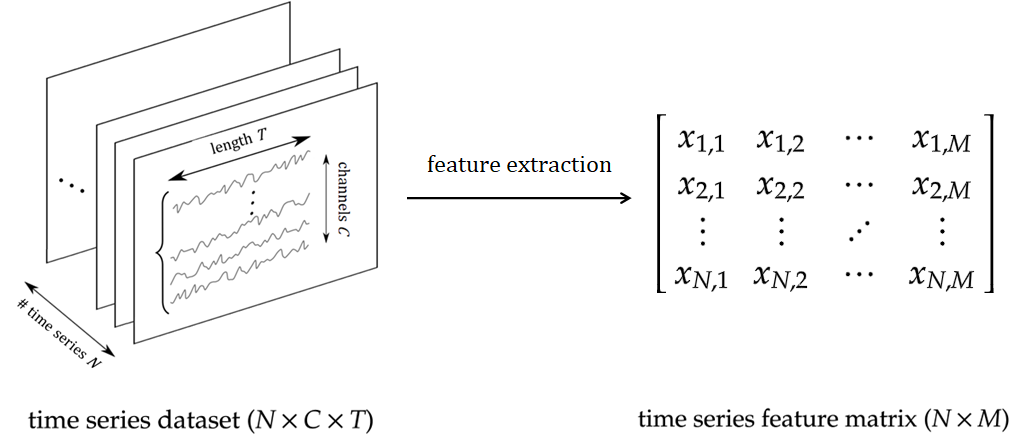
\includegraphics[width=\textwidth]{images/ts_feat_extr}
    \caption{Time series feature extraction}
    \label{fig:ts_feat_extr}
\end{figure}

Time series data differs from static data, which instead is not characterized by a temporal dimension. Since measurements in a time series are correlated in the temporal dimension, generally we cannot use feature extraction techniques commonly used for static datasets, as they are typically not able to capture temporal relationships in data \cite{ts_feat_extr}.

Time series feature extraction methods can be categorized into:
\begin{itemize}
    \item Manual feature extraction: features are hand-crafted by a domain expert to capture relevant information of a specific problem. These domain-specific features are very relevant and discriminative for the problem at hand, but are often poorly generalizable to other regression problems.
    \item Automatic feature extraction: features are automatically extracted by an algorithm, in a supervised or unsupervised fashion (i.e. with or without the knowledge of the label associated to each time series in the dataset). Automatic feature extraction has the advantage of not requiring expertise of the data.
\end{itemize}

The majority of scientific papers on SOH estimation of Li-ion battery cells profusely exploit hand-engineered features \cite{tesi_filippo, manual_extr_soh_2, manual_extr_soh_3, manual_extr_soh_4, manual_extr_soh_5, manual_extr_soh_6, manual_extr_soh_7, manual_extr_soh_8, manual_extr_soh_9, manual_extr_soh_10, manual_extr_soh_11, manual_extr_soh_12, manual_extr_soh_13}, but recent developments point in the direction of automatic feature learning and extraction based on deep convolutional neural networks \cite{auto_extr_soh_1, auto_extr_soh_2, auto_extr_soh_3, auto_extr_soh_4, auto_extr_soh_5}; in the latter approach, the feature extraction step is integrated in the convolutional part of the network (meaning that feature extraction and model training are performed in parallel).

In this thesis work, automatic approaches to feature extraction are explored. Specifically, a recent domain-agnostic unsupervised feature extraction method called \textsc{MiniRocket} is studied (sec. \ref{sec:minirocket}) and applied to our SOH estimation problem. Moreover, a novel computationally-inexpensive feature extraction method has been developed (sec. \ref{sec:my_method}) and applied, achieving surprisingly high performance on a synthetic dataset of monitoring data. The two estimation strategies are thoroughly compared in sec. \ref{sec:results}.





\section{Feature extraction through \textsc{MiniRocket}}
\label{sec:minirocket}
In 2020, Dempster et al. \cite{rocket} proposed \textsc{Rocket}, a new time series classification procedure that achieves state-of-the-art accuracy in TSC with a low computational expense. \textsc{Rocket} consists of two parts: an unsupervised feature extraction step which transforms time series using a large number of random convolutional kernels, and a classification step with a classification model of choice (by default a ridge regression classifier).
One year later, the same authors reformulated \textsc{Rocket} into a new classification method, called \textsc{MiniRocket} (for \textbf{MINI}mally \textbf{R}and\textbf{O}m \textbf{C}onvolutional \textbf{KE}rnel \textbf{T}ransform) \cite{minirocket}. It is up to 75 times faster than \textsc{Rocket}, while being almost fully deterministic and maintaining essentially the same performances on TSC tasks.

By replacing \textsc{MiniRocket}'s classification model with a regression model, \textsc{MiniRocket} becomes a time series regression algorithm, which is able to achieve state-of-the-art performances in TSER problems \cite{TSER}.

We will now briefly describe how \textsc{MiniRocket}'s feature extraction step works when dealing with univariate time series datasets. A naive extension to multivariate time series is then described.



\subsection{Convolution}
\label{sec:convolution}
Convolution is a widely used transformation applied to a matrix, which consists in computing a locally weighted sum of its elements with weights given by a matrix called \textit{kernel}.

\begin{definition}[Discrete 2D convolution]
Given a matrix $X \in \mathbb{R}^{n\times m}$ (called \textit{input feature map}) and a matrix $W \in \mathbb{R}^{h\times k}$ (called \textit{convolutional kernel}), the discrete 2D convolution (or simply convolution) between $X$ and $W$ is the matrix $Z$ (called \textit{output feature map}) whose elements are given by the following operation
\[
Z(i,j) = (X*W)(i,j) = \sum_{r=1}^h \sum_{s=1}^k X(i+s-1, j+r-1) W(r, s)
\]
\end{definition}
Usually, a bias value $b\in\mathbb{R}$ is added to the convolution output in many applications.

\begin{remark}
When $m=k=1$, the discrete convolution becomes 1-dimensional. This is the operation applied to univariate time series (which can be thought of as $1\times T$ matrices, or equivalently as vectors of length $T$).
\end{remark}

Convolution has a simple visual interpretation, visualized in fig. \ref{fig:convolution}: the kernel matrix "slides" over the input feature map vertically and horizontally, locally identifying a submatrix on the input feature map of the same shape as the kernel; the elements of the output feature map are computed by taking the element-wise product of the kernel and said submatrix and summing them.

\begin{figure}
    \centering
    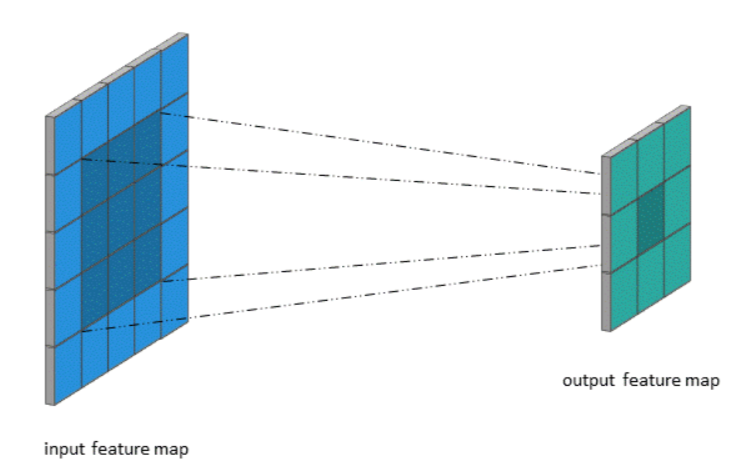
\includegraphics[width=0.6\textwidth]{images/convolution}
    \caption[Discrete convolution]{A visual representation of a discrete 2D convolution between a $5\times5$ input feature map and a $3\times3$ kernel. Taken from \cite{conv_fig}}
    \label{fig:convolution}
\end{figure}

In many applications, richer variants of the convolution operation are used, which employ the techniques of \textit{zero-padding} and \textit{dilation} \cite{dl_book}:

\begin{itemize}
\item Zero-padding (or simply padding) consists in concatenating rows/columns full of zeros at the beginning or the end of an input feature map, prior to applying convolution. typically, the number of leading and trailing rows/columns added is the same ($p$). A zero-padded convolution is visualized in fig. \ref{fig:padded_conv}
\item Dilation consists in "spreading" a kernel over the input feature map, such that with a dilation parameter of $d$ the weights in a kernel are convolved with every $d$-th element of an input feature map along each direction. A dilated convolution is visualized in fig. \ref{fig:dilated_conv}.
\end{itemize}

\begin{figure}[htb!]
\centering
\begin{subfigure}[t]{0.45\textwidth}
    \centering
    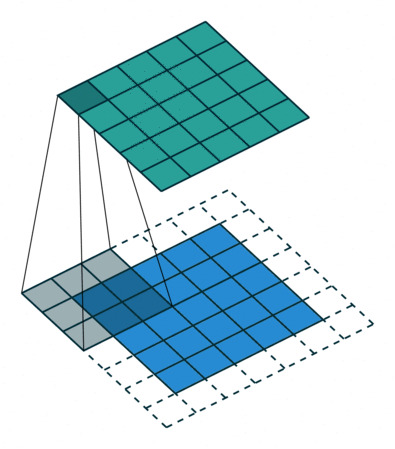
\includegraphics[width=\textwidth]{images/padded_conv}
    \caption[Zero-padded convolution]{Zero-padded convolution with padding parameter $p=1$}
    \label{fig:padded_conv}
\end{subfigure}
\hfill
\begin{subfigure}[t]{0.45\textwidth}
    \centering
    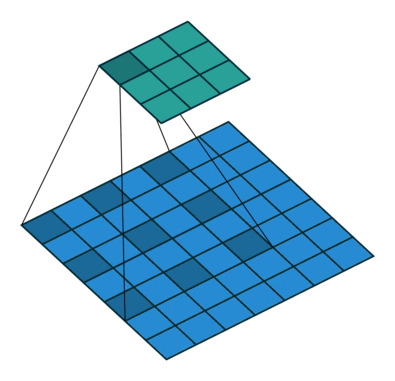
\includegraphics[width=\textwidth]{images/dilated_conv}
    \caption[Dilated convolution]{Dilated convolution with dilation parameter $d=2$}
    \label{fig:dilated_conv}
\end{subfigure}
\caption[Variants of the convolution operation]{Variants of the convolution operation between a $5\times5$ input feature map and a $3\times3$ kernel. Taken from \cite{conv_variants_fig}}
\label{fig:conv_variants}
\end{figure}



\subsection{Fitting \textsc{MiniRocket}'s feature extractor}
\label{sec:minirocket_feat_extr}


\paragraph{Length}
\textsc{MiniRocket} uses a fixed set of 84 kernels of length 9, with weights restricted to two values. These 84 kernels are selected a priori among the $2^9=512$ possible two-valued kernels of length 9. Using such a low number of kernels helps in keeping the computational cost low enough while not hampering performances.


\paragraph{Weights}
The 84 chosen kernels have weights restricted to two values: $\alpha=-1$ and $\beta=2$. This choice is made arbitrarily by the authors, in the sense that the scale of these values is unimportant, as bias values are drawn from the convolution output (as discussed in the next paragraph) and so they match its very scale. Thus, it is not necessary to normalise the input time series.

Moreover, the number of -1s is double the number of 2s in all 84 kernels, such that the sum of the weights of a kernel is 0. This ensures that the kernels are sensitive only to the \textit{relative} magnitude of the input values, i.e. that the convolution output is invariant to the addition or subtraction of any constant value to the input: $X*W = (X\pm c)*W$.

The position of the three $\beta=2$ weights inside each of the 84 kernels is defined by the sequence $[(1,2,3), (1,2,4), \dots, (6,8,9), (7,8,9)]$.


\paragraph{Bias}
Bias values associated to each kernel/dilation combination are used in computing PPV features, as discussed in the associated paragraph.
For a given kernel $W$ and dilation parameter $d$ (in short: $W_d$), bias values are drawn from the quantiles of the convolution output between $W_d$ and a randomly selected time series $X_i$ in the dataset. The orders of the quantiles assigned to each $W_d$ are computed deterministically with the following low-discrepancy sequence
\begin{equation}
i\cdot\frac{1+\sqrt{5}}{2}\text{ mod }1,\;\forall i\in [1,2,\dots,n]
\end{equation}
where $n$ is the total number of desired PPV features to be extracted.

The number of biases to use with each kernel/dilation combination $W_d$ (or, equivalently, the number of features that are extracted from the convolution output with kernel/dilation $W_d$) depend on $d$ and on the length $l$ of the time series $X$, as discussed in the next paragraph.

Drawing at random a time series $X_i$ for the purpose of sampling the bias values is the only stochastic element of \textsc{MiniRocket}; remaining parameters either depend solely on the time series length or are intended to be kept at their default values.


\paragraph{Dilation}
Possible dilation for each kernel values are in the range
\begin{equation}
D=\{\floor{2^0},\floor{2^{\text{max}/m}},\floor{2^{2\cdot\text{max}/m}},\dots,\floor{2^{m\cdot\text{max}/m}}\}
\end{equation}
where $m$ is the maximum possible number of dilations per kernel (set to 32 by default) and $\text{max}=\log_2(l-1)/8$ is the largest possible dilation parameter for a kernel of length $9$ applied to a time series of length $l$ (i.e. such that the \textit{effective} length of the dilated kernel of length $9$ is exactly $l$).

The count of each unique integer dilation value in $D$ determines the number of PPV features to be computed per dilation (scaled according to the total number of desired PPV features, $n$, so that the sum of the scaled counts equals $n$), ensuring that exponentially more features are computed for smaller dilations.


\paragraph{Padding}
Zero-padding is applied alternately every other kernel/dilation combination such that, overall, half the combinations use padding and half do not. The number of leading and trailing zeros added to the time series is set in such a way that the convolution operation begins with the middle (5th) weight of a kernel centered on the first measurement of the time series and ends with the middle weight centered on the last measurement.


\paragraph{Features}
The feature extracted by \textsc{MiniRocket} from each time series $X$ for each kernel/dilation combination $W_d$ and each bias $b$ is the proportion of convolution output values which are greater than $b$:
\begin{equation}
\text{PPV}(X*W_d, b) \coloneqq \frac{1}{n_\text{out}} \sum\left[X*W_d > b\right]
\end{equation}
where $n_\text{out}$ denotes the number of elements of the convolution output vector $X*W_d$ and $[\mathbf{x}\in a]$ denotes the indicator function. PPV stands for \textit{proportion of positive values}.

By default, \textsc{MiniRocket} represents each time series with a total of 9,996 PPV features (i.e. the nearest multiple of 84 -- the number of kernels -- less than 10,000).


\subsection{\textsc{MiniRocket} for multivariate time series}
\label{sec:multivariate-minirocket}
The authors \cite{minirocket} also extended \textsc{MiniRocket} to multivariate time series in a basic way\footnote{The explanation of multivariate \textsc{MiniRocket} given in this section is based only on the code implemented by the authors (which can be found at \url{https://github.com/angus924/minirocket/blob/main/code/minirocket_multivariate.py}), as the extension to multivariate time series is not mentioned anywhere in the original paper \cite{minirocket}.}.

Suppose that the time series in the dataset have $C$ channels. For each kernel/dilation combination, a random subset of $k = \floor{2^{\mathcal{U}(0,M)}}$ out of $C$ channels is taken, where $M = \log_2(\min(C,9)+1))$ and $\mathcal{U}(0,M)$ means taking a random sample from the uniform distribution on $(0,M)$.\footnote{$k$ is distributed according to the floor of a log-uniform distribution on $[1,M]$.

A random variable $X$ is distributed according to a log-uniform distribution with support on $[a,b]$ if $\ln{(X)}\sim\mathcal{U}(ln(a),ln(b))$, where $\mathcal{U}$ indicates the uniform distribution. \cite{loguniform}

Suppose now that $a,b\in\mathbb{N}$; it can be proved that $\floor{X}$ is a discrete random variable with support on $\{a, a+1, \dots, b-1\}$ with probability mass function
\[
p(n) = \ln\left(\frac{n+1}{n}\right) / \ln\left(\frac{b}{a}\right)
\]
E.g.: when sampling a random subset of $k$ out of $C=3$ channels from a multivariate time series, with $k$ distributed according to the above distribution, the probability masses of $k$ are: $p(1)=0.5$, $p(2)=0.292$, $p(3)=0.208$. Therefore, smaller subsets are more likely to be extracted.
}

When drawing the biases for each kernel/dilation combination, kernel $W_d$ is convolved with each of the $k$ channels of $X$ that have been randomly selected; then, the $k$ convolution outputs are summed, and this vector is used to draw the biases with the procedure already discussed in sec. \ref{sec:minirocket_feat_extr}.

This variant of \textsc{MiniRocket}'s feature extractor for multivariate time series "suffers" from at least two drawbacks with respect to the original, univariate version:
\begin{itemize}
\item A new stochastic element is added: the random sampling of the channels of the time series to be used in the feature extraction, for each kernel/dilation combination.
\item The different channels of a time series do not have the same mean and standard deviation in general. Since the sum of several convolution outputs is taken, the time series channels must be normalized for this method to make sense mathematically (whereas original \textsc{MiniRocket} doesn't require time series to be normalized, as discussed in sec. \ref{sec:minirocket_feat_extr}).
\end{itemize}



\section{Feature selection with PCA}
\label{sec:pca}
Dealing with high-dimensional datasets (i.e. datasets with a large number of predictors) is often undesirable. Many machine learning models do not scale well to high-dimensional datasets due to sparseness in data (a phenomenon known as \textit{curse of dimensionality}) and generally high computational cost. Moreover, predictors have some degree of mutual dependence in many experimental settings. For these reasons, it is often desirable to perform a \textbf{dimensionality reduction} of the data \cite{dim_red}.

\textbf{Principal Components Analysis} (PCA) \cite{pca} is a method for performing a particular change of basis on the data, in which the axes of the new coordinate system are the set of orthonormal eigenvectors of the scatter matrix $A=X^TX$, commonly known as "principal components" of the dataset $X$. PCA is typically exploited as an unsupervised dimensionality reduction technique, since it has the nice property of maximizing the variance of the data when mapped down to lower dimensional spaces.

The PCA problem can be expressed in many different ways, which can be proven to be equivalent. One of the most interesting statements is the following one.

Given a dataset $X\in\mathbb{R}^{N\times M}$, with data points $\mathbf{x}_1, \dots, \mathbf{x}_N$, and assuming that data is zero-centered ($\frac{1}{N}\sum_{i=1}^N \mathbf{x}_i = 0$), find a set of $D \leq M$ orthonormal directions $\mathbf{w}_1,\dots,\mathbf{w}_D$ by solving consecutively the following variance maximization problems:
\begin{align}
\begin{split}
\argmax_{\mathbf{w}_1:\norm{\mathbf{w}_1}=1} \quad & \frac{1}{N}\sum_{i=1}^N(\langle\mathbf{w}_1,\mathbf{x}_i\rangle)^2\\
\argmax_{\substack{\mathbf{w}_k:\norm{\mathbf{w}_k}=1 \\ \mathbf{w}_kA\mathbf{w}_j=0, \; j=1,\dots,k-1}} \; & \frac{1}{N}\sum_{i=1}^N(\langle\mathbf{w}_k,\mathbf{x}_i\rangle)^2, \qquad k=2,\dots,D
\end{split}
\end{align}

This problem is solved by choosing $\mathbf{w}_1=\mathbf{u}_1,\dots,\mathbf{w}_D=\mathbf{u}_D$, where $\mathbf{u}_1,\dots,\mathbf{u}_D$ are the unit-norm eigenvectors associated to the largest $D$ eigenvalues of the scatter matrix $A$; the maximum values of the objective functions of each problem are, in order, $\lambda_1,\dots,\lambda_D$.

This formulation is of particular interest because of the following interpretation: $\mathbf{w}_1$ is the direction of a line onto which the variance of the projected points, $\langle\mathbf{w}_1,\mathbf{x}_i\rangle$, is maximized; $\mathbf{w}_2$, is a second direction which maximizes the variance of $\langle\mathbf{w}_2,\mathbf{x}_i\rangle$ but which is also orthogonal to $\mathbf{w}_1$ (i.e., the projected points onto $\mathbf{w}_1$ and $\mathbf{w}_2$ are uncorrelated); and so on with the remaining maximization problems, which yield other directions of variance maximization which are orthogonal to all the previously found directions. This interpretation is particularly evident in fig. \ref{fig:pca}

\begin{figure}[htb!]
    \centering
    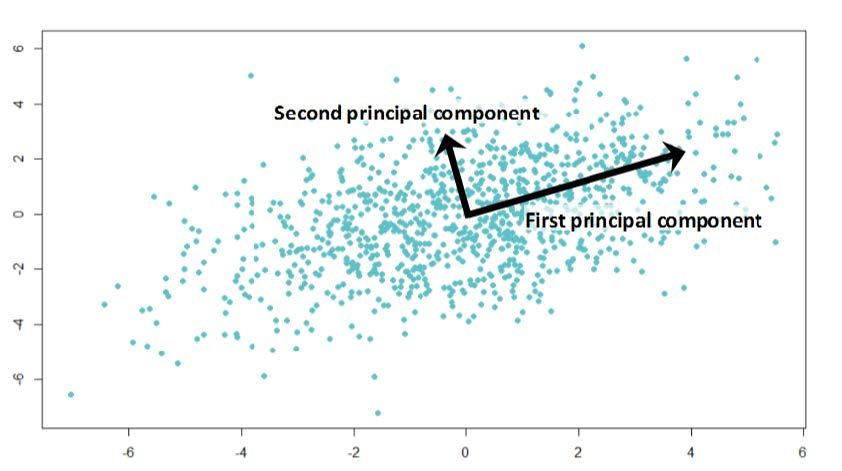
\includegraphics[width=\textwidth]{images/pca}
    \caption[PCA on a 2D dataset]{PCA on a simple 2D dataset. Taken from \cite{pca_img}}
    \label{fig:pca}
\end{figure}

The proportion of the variance represented (or "\textit{explained}") by each eigenvector can be calculated by dividing the eigenvalue corresponding to that eigenvector by the sum of all eigenvalues. This means that by reducing dimensionality with $D$ principal components, the proportion of variance explained by these is $\sum_{i=1}^D \lambda_i / \sum_{i=1}^M \lambda_i$.

Performing dimensionality reduction through PCA is especially useful when using \textsc{MiniRocket} as a feature extractor, since it produces a very large number of features (9,996) from each input time series.





\section{Feature extraction through linear regression in the V-I-SOC space}
\label{sec:my_method}
\textsc{MiniRocket} is a domain-agnostic feature extractor, meaning that it could be effective in many different experimental contexts. However, embedding a SOH estimation method on an EV requires that the procedure has a low memory footprint and -- most critically --
a limited computational cost, due to the need of estimating the SOH in real-time. When performing a SOH prediction, \textsc{MiniRocket} computes almost 10,000 convolutions between the time window of monitoring data given as input and the \textsc{MiniRocket} kernels. As the length of the time windows increase, computing so many convolutions becomes infeasible for the computational devices embedded on a typical BMS of an EV.

In this section, a new feature extraction method is introduced. This method is:
\begin{itemize}
    \item domain-specific: this method is specifically designed for the task of estimating an EV battery pack's SOH; it leverages only on the voltage (V), current (I) and SOC measurements recorded during a driving session and takes the shape of their data distribution into account;
    \item computationally cheap: for each time window of monitoring data, a simple multivariate linear regression model is fitted, an operation which requires only a limited amount of computation;
    \item low dimensional: from each time window of monitoring data only 3 features are extracted.
\end{itemize}

Some preliminary definitions are introduced in order to more easily explain how this method works.

EV field data typically consists of time series of V, I, SOC measurements (among others), taken during a driving session of the vehicle. From now on, we will refer to the tuple of measurements $(\text{V}(t_i), \text{I}(t_i), \text{SOC}(t_i))$ at a timestamp $t_i$ as an \textbf{operating point} of the EV.

The first key observation in the design of this novel procedure is that the operating points observed on a certain driving session seem to lie on a hyperplane in the V-I-SOC space. This observation is very accurate in relation to synthetic data (fig. \ref{fig:visoc_synth1} and \ref{fig:visoc_synth2}), but it is also true for real monitoring data with a certain degree of approximation (fig. \ref{fig:visoc_real1} and \ref{fig:visoc_real2}).

\begin{figure}[htb!]
\centering
\begin{subfigure}[t]{0.475\textwidth}
    \centering
    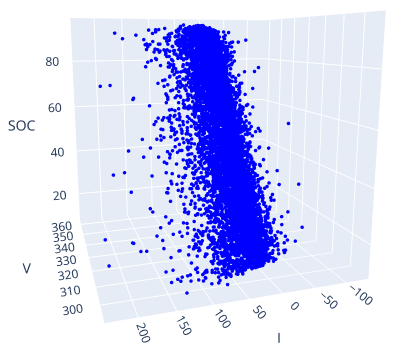
\includegraphics[width=\textwidth]{images/visoc_synth1}
    \caption{}
    \label{fig:visoc_synth1}
\end{subfigure}
\hfill
\begin{subfigure}[t]{0.475\textwidth}
    \centering
    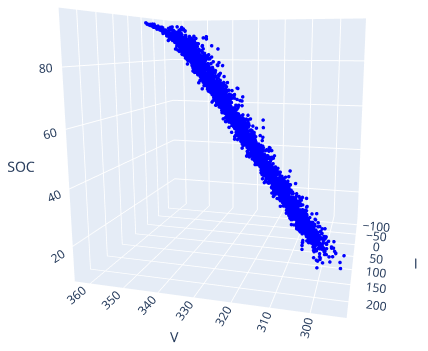
\includegraphics[width=\textwidth]{images/visoc_synth2}
    \caption{}
    \label{fig:visoc_synth2}
\end{subfigure}
\vskip\baselineskip
\begin{subfigure}[t]{0.475\textwidth}
    \centering
    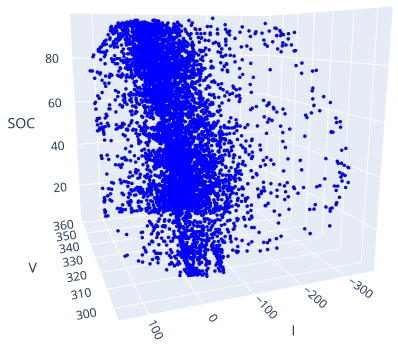
\includegraphics[width=\textwidth]{images/visoc_real1}
    \caption{}
    \label{fig:visoc_real1}
\end{subfigure}
\hfill
\begin{subfigure}[t]{0.475\textwidth}
    \centering
    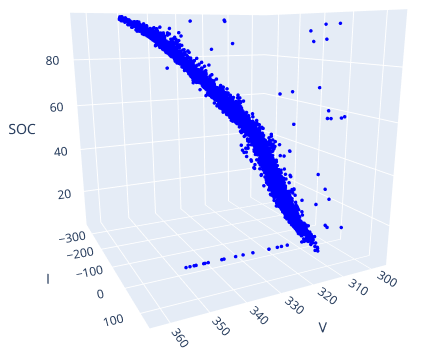
\includegraphics[width=\textwidth]{images/visoc_real2}
    \caption{}
    \label{fig:visoc_real2}
\end{subfigure}
\caption[Synthetic and real operating points associated to the same SOH level]{Operating points associated to the same SOH level, randomly extracted from: (a)-(b) synthetic dataset (sec. \ref{sec:ds_gen}), (c)-(d) real dataset (chap. \ref{sec:aviloo_ds}).}
\label{fig:visoc}
\end{figure}

The particular hyperplane defined by the operating points seems to independent of the particular drive cycle, but interestingly it seems to be discriminative of the age of the battery during that driving session. In fact, the second key observation is that different battery SOH values define different hyperplanes in the V-I-SOC space. This is highlighted in fig. \ref{fig:visoc_soh_planes}.

\begin{figure}
    \centering
    \hspace{-1cm}
    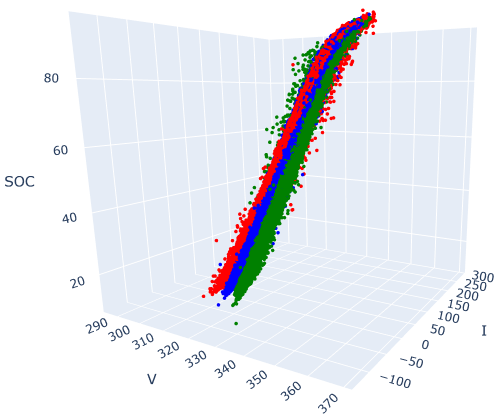
\includegraphics[width=0.7\textwidth]{images/visoc_soh_planes}
    \caption[Synthetic Operating points associated to different SOH levels]{Operating points associated to different SOH levels (red: 100\%, green: 90\%, blue: 80\%), randomly extracted from the synthetic dataset.}
    \label{fig:visoc_soh_planes}
\end{figure}

Therefore, we may argue that the problem of predicting the SOH of a battery pack is equivalent to the task of finding the hyperplane which approximates all the possible operating points of an EV at a specific point of its operating lifetime.

To make this task compatible with the requirements of a real-time SOH estimation method, we need to find said hyperplane from the knowledge of only a relatively short time window of operating points (i.e. a small sample of consecutive operating points) instead of the whole statistical population of operating points.

The equation of an affine hyperplane in a three-dimensional space is
\begin{equation}
    z=ax+by+c
\end{equation}
A 3D hyperplane is uniquely identified by its three parameters $a, b, c \in \mathbb{R}$.

Therefore, we can represent a time window of operating points with just three features, namely the $a, b, c$ parameters defining the hyperplane which better "describes" those operating points.

Estimating the parameters of the hyperplane which passes near all the points in a given set can be stated as a linear regression problem \cite{hastie}.
\begin{definition}[Multiple linear regression model]
\label{def:linear_model}
Let $\mathbf{x}=(x_1,\dots,x_M) \in \mathbb{R^M}$. A multiple linear regression model (or simply linear model) is a function of the form
\[
f(\mathbf{x};\bm{\beta}) = \beta_0 + \sum_{i=1}^M \beta_i x_i
\]
\end{definition}
In many experimental contexts, a linear model is a reasonable approximation of the relationship between an output variable $y$ and an input vector $\mathbf{x}$.

The problem of estimating the parameters $\bm{\beta}$ of a linear model from a set of training data $(\mathbf{x}_{1},y_1),\dots,(\mathbf{x}_{n},y_n)$ is called \textit{linear regression problem}. There exists many estimation methods for solving the linear regression problem. Two such methods have been explored for designing our novel feature extractor: ordinary least squares estimation (sec. \ref{sec:ols}) and Theil-Sen estimation (sec. \ref{sec:theil-sen}).

\subsection{Ordinary least squares estimation}
\label{sec:ols}
Ordinary least squares (OLS) estimation is the most common solver for a linear regression problem. It consists in finding the parameters $\bm{\beta}$ minimizing the residual sum of squares
\begin{equation}
\text{RSS}(\beta) = \sum_{i=1}^N (y_i - f(\mathbf{x}_{i};\bm{\beta}))^2
\end{equation}

Let $X$ the $N\times M+1$ matrix having the dataset samples $\mathbf{x}_{1},\dots,\mathbf{x}_{N}$ as rows, with a constant $x_{i,0}=1$ prepended to each row to account for the bias term, and let $\mathbf{y} = (y_1,\dots,y_N)^T$. The analytical expression of the RSS can be rewritten as
\begin{equation}
\text{RSS}(\bm{\beta}) = \norm{\mathbf{y}-X\bm{\beta}}^2 = (\mathbf{y}-X\bm{\beta})^T(\mathbf{y}-X\bm{\beta})
\end{equation}

If the Gram matrix $X^T X$ is positive definite, then the OLS regression problem has a unique solution:
\begin{equation}
\hat{\bm{\beta}}^{OLS} = (X^TX)^{-1}X^T\mathbf{y}
\end{equation}

The OLS method is visualized in fig. \ref{fig:ols}.

\begin{figure}[hbt!]
    \centering
    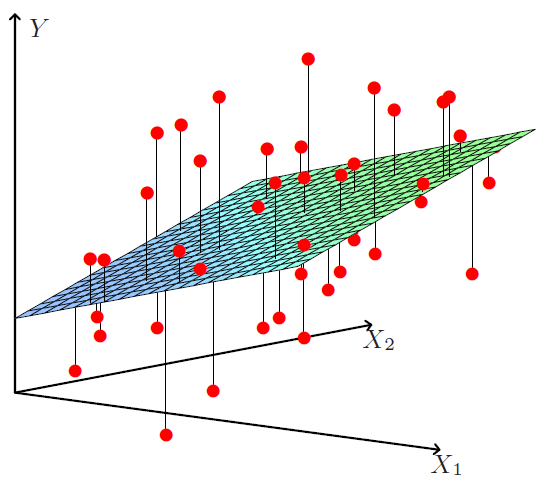
\includegraphics[width=0.7\textwidth]{images/ols}
    \caption[Fitting a linear model via OLS]{Fitting of a linear model on a 2D dataset by ordinary least squares estimation. We seek the linear function of $\mathbf{x}$ that minimizes the sum of squared residuals from $y$. Taken from \cite{hastie}}
    \label{fig:ols}
\end{figure}

OLS generally yields a good estimate for the parameters $\bm{\beta}$ under the assumption that $\mathbb{E}(y|\mathbf{x})$ is a linear function with good approximation. However, OLS estimates are highly sensitive to outliers, since it seeks to minimize all residuals equally and penalizes large residuals more (due to squaring) \cite{robust_regr}. In many experimental contexts the available data is contaminated by outliers, which for instance arise from measurement errors due to sensors (as is often the case in EV monitoring data), approximation errors (as is the case when resampling EV monitoring data to a common time base for all the signals through linear interpolation) or even unavoidable sampling error (which in the EV context is due to the fact that sensors monitor continuous signals by collecting them at a specific sampling rate, therefore often neglecting their sudden high-frequency variations).

Robust regression methods \cite{robust_regr} are designed to limit the effect that the presence of outliers has on regression estimates.

\subsection{Theil-Sen estimation}
\label{sec:theil-sen}
Theil-Sen (TS) estimation method is a robust alternative to the OLS method that reduces outliers' contribution to the error loss, thereby limiting their impact on regression estimates.

TS estimation was first introduced by Henri Theil \cite{theil} and Pranab K. Sen \cite{sen} as a method for fitting simple linear models (i.e. models with just one explanatory variable, $f(x;m,b)=mx+b$); recently, it has been generalized to multiple linear regression by Dang et al. \cite{multi_theil-sen}.

\subsubsection{Theil-Sen estimation for simple linear models}
As originally defined by Theil \cite{theil}, the TS estimate for the slope parameter $m$ of the simple linear model on a set of two-dimensional points $(x_1,y_1),\dots,(x_N,y_N)$ is the median of the slopes $m_{i,j} = (y_j - y_i)/(x_j - x_i)$ determined by all pairs of sample points. Sen \cite{sen} extended this definition to handle the case in which two data points have the same $x$ coordinate, by taking the median of the slopes determined only by pairs of points having distinct $x$ coordinates. The intercept $b$ can be estimated in a number of ways; one of them is setting $b$ as the median of the values $b_i = y_i - \hat{m}^{TS}x_i$.

It is clear that computing $\hat{m}^{TS}$ and $\hat{b}^{TS}$ with this procedure becomes very expensive as the dataset size $N$ increases: for $N$ points, $\binom{N}{2} = \frac{N(N-1)}{2}$ slopes must be computed -- one for each pair of points.

One possible solution is sampling at random a subpopulation $S \ll \binom{N}{2}$ of pairs of points and performing Theil-Sen estimation on this reduced training set, effectively computing only $S$ slopes. This has the effect of reducing the computational cost, but the estimation may become very sensitive to the particular random choice of the subpopulation, especially if $S$ is very small. This variant of the Theil-Sen method is implemented in the Python library scikit-learn, where $S$ is set with the hyperparameter \texttt{max\_subpopulation} \cite{sklearn_theil-sen}. In this thesis work, $S$ has been set to 10,000 for all experiments.

The Theil–Sen estimator is an unbiased estimator for the true slope $m$ \cite{sen, unbiasedness_theil-sen}, has high asymptotic efficiency \cite{sen, efficiency_theil-sen} and is more robust to outliers than OLS estimator \cite{multi_theil-sen}. In its original formulation (simple linear regression and $S=\binom{N}{2}$), it has a breakdown point of 29.3\%, meaning that it can tolerate arbitrary corruption of up to 29.3\% of the input data points without degradation of its accuracy.

A visual comparison between OLS and Theil-Sen estimation applied to a simple 2D dataset with outliers is reported in fig. \ref{fig:theil-sen_vs_ols}.
\begin{figure}[hbt!]
    \centering
    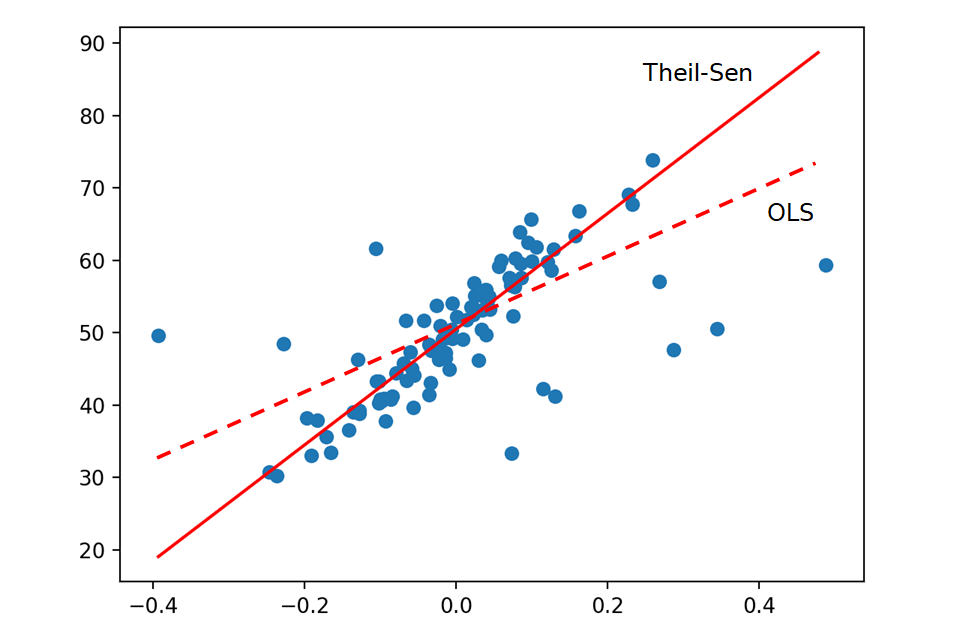
\includegraphics[width=0.8\textwidth]{images/theil-sen_vs_ols}
    \caption[Fitting a simple linear model via TS]{Fitting a simple linear regression model via Theil-Sen estimation vs ordinary least squares. Adapted from \cite{theil-sen_vs_ols}}
    \label{fig:theil-sen_vs_ols}
\end{figure}

On a final note, there is no closed form solution for TS estimates, as opposed to OLS; the algorithmic nature of TS method makes it well-suited for a computer implementation.

\subsubsection{Theil-Sen estimation for multiple linear models}
Recently, Dang et al. \cite{multi_theil-sen} extended Theil-Sen estimation to multiple linear regression.

Consider a multiple linear regression model $f(\mathbf{x};\bm{\beta}) = \bm{\beta}\mathbf{x}$ (where, as usual, $\bm{\beta},\mathbf{x} \in \mathbb{R}^{M+1}$ and $x_{i,0}=1$). The hyperplane defined by the regression parameters $\bm{\beta}$ is determined by exactly $M+1$ points. Similarly to the simple regression case, we can consider a (random) subpopulation of $S\leq \binom{N}{M+1}$ subsets of $M+1$ points ($\mathbf{k}_1, \dots, \mathbf{k}_S$) and compute the unique $\bm{\beta}^{(i)}$ associated to each $\mathbf{k}_i$ by solving the associated OLS problem\footnote{Note that the OLS problem with exactly $n$ points in a $n$-dimensional space is trivially equivalent to finding the (unique) hyperplane passing through those $n$ points.}:
\begin{equation}
\bm{\beta}^{(i)} = (X^{(i)T} X^{(i)})^{-1} X^{(i)T} \mathbf{y}
\end{equation}
where $X^{(i)}$ is the matrix whose rows are the vectors $\mathbf{x}_{j} \in \mathbf{k}_i$. Notice that with this procedure the "slope vector" $(\beta_1^{(i)},\dots,\beta_{M+1}^{(i)})$ and the intercept $\beta_0^{(i)}$ are computed simultaneously.

After having computed $\bm{\beta}^{(1)},\dots,\bm{\beta}^{(S)}$, the Theil-Sen estimate for $\bm{\beta}$ is their sample spatial median \cite{spatial_median}
\begin{equation}
\hat{\bm{\beta}}^{TS} = \text{\textsc{SpatialMedian}}(\bm{\beta}^{(1)},\dots,\bm{\beta}^{(S)})
\end{equation}
For reference, the sample spatial median is discussed in appendix \ref{sec:spatial_median}

Multiple Theil-Sen estimation (MTS) is still robust to outliers, although a bit less than its simple counterpart, with a breakdown point of $1-(1/2)^{1/(M+1)}$. E.g.: for $M+1=3$, as in our experimental setting (see chap. \ref{sec:experiments}), the breakdown point is 20.6\%.





\section{Regression models}
\label{sec:regr_models}
Upon transforming a time series dataset to its static feature-based representation, we must choose and train a regression model to predict the SOH. A huge amount of regression models exist, both linear and non-linear; in this thesis work, we experiment with three well-known regression models: ridge regression (sec. \ref{sec:ridge}), random forest (sec. \ref{sec:random_forest}), feed-forward neural network (sec. \ref{sec:neural_network}).



\subsection{Ridge regression}
\label{sec:ridge}
Consider once more the linear regression model (def. \ref{def:linear_model}). In some cases, the Gram matrix $X^T X$ is singular or nearly-singular: this happens in particular when there are multicollinear (i.e. highly correlated) independent variables in the data. Because the OLS estimates depend upon $(X^T X)^{-1}$, when $X^T X$ is nearly-singular the OLS estimation problem becomes ill-posed, and this may lead to serious numerical problems, namely estimates exhibiting high variance\footnote{For instance, let us suppose that a dataset has two independent variables "weight" and "height" and one dependent variable "age". It is reasonable to assume that weight and height have a strong linear correlation. When fitting a linear model to the dataset via OLS, we may end up with a very large positive coefficient for the weight and a similarly very large negative coefficient for height.}.
To mitigate this problem, we may impose a size constraint on the coefficients by introducing a L2 regularization term in the residual sum of squares:
\begin{equation}
\text{RSS}_\text{L2}(\bm{\beta};\lambda) = \sum_{i=1}^N (y_i - f(\mathbf{x}_{i};\bm{\beta}))^2 + \lambda \sum_{i=1}^M \beta_i^2
\end{equation}
or, in matrix form:
\begin{equation}
\text{RSS}_\text{L2}(\bm{\beta};\lambda) = (\mathbf{y}-X\bm{\beta})^T(\mathbf{y}-X\bm{\beta}) + \lambda \bm{\beta}^T I_0 \bm{\beta}
\end{equation}
where $I_0$ is the $(M+1) \times (M+1)$ identity matrix with 0 as the first diagonal entry (i.e. $(I_0)_{1,1}=0$) and  $\lambda\in\mathbb{R}$ is a user-defined penalty factor (the larger, the stronger the penalization of large coefficients, as shown in fig. \ref{fig:ridge_penalty}).

\begin{figure}[hbt!]
    \centering
    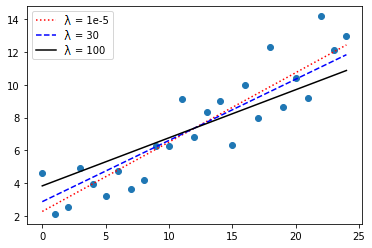
\includegraphics[width=0.8\textwidth]{images/ridge_penalty}
    \caption[Choice of the penalty factor in RR]{The effect of the choice of the penalty factor $\lambda$ on the solution of the ridge regression problem. Adapted from \cite{ridge_penalty}}
    \label{fig:ridge_penalty}
\end{figure}

Note that the intercept $\beta_0$ is left out of the penalty term, as penalizing the intercept would make the procedure dependent on the scale of $\mathbf{y}$.

The linear regression problem solved by minimizing the L2-regularized RSS above is called \textbf{ridge regression} problem \cite{ridge, hastie}.
Ridge regression has the following closed form solution
\[
\hat{\bm{\beta}}^\text{ridge} = (X^TX+\lambda I_0)^{-1}X^T\mathbf{y}
\]

As we can observe, a positive constant is added to the diagonal of $X^TX$ before inversion: this makes the resulting matrix non-singular even when $X^TX$ is, thus making the linear regression problem well-conditioned. Notice also that due to the addition of $\lambda I_0$ ridge estimates are not equivariant under scaling of the inputs (as opposed to OLS), and so one normally standardizes the dataset before solving the ridge regression problem.

In many experimental contexts, $X$ is a very large matrix. In such cases, the matrix $X^TX$ and the inverse of $X^TX+\lambda I_0$ are very expensive to compute. For this reason, when $N$ and/or $M$ are particularly large, the ridge regression problem is solved iteratively via SGD (sec. \ref{sec:sgd}).





\subsection{Random forest}
\label{sec:random_forest}
\textbf{Random forest} \cite{random_forest, hastie} is an ensemble learning method for classification and regression tasks, which performs prediction through majority voting (classification) or averaging (regression) the predictions of an ensemble of decision trees. In this section, we will discuss only random forest regression.

A regression tree is a simple regression model that predicts the response variable $y$ associated to a sample $\mathbf{x}$ by traveling from its \textit{root node} to one of its \textit{leaves}. At each node on the root-to-leaf path, the successor node is chosen on the basis of a splitting of the input space. Usually, the splitting is a binary "test" on one of the features of $\mathbf{x}$. In this way, a decision tree tesselates the input space with non-overlapping hyper-rectangles ("boxes") in which a certain number ($\geq1$) of training samples are located. A prediction is made by averaging the ground-truth labels of the training samples located in the input space box associated to the leaf reached. An example is shown in fig. \ref{fig:regr_tree}.

\begin{figure}[hbt!]
    \centering
    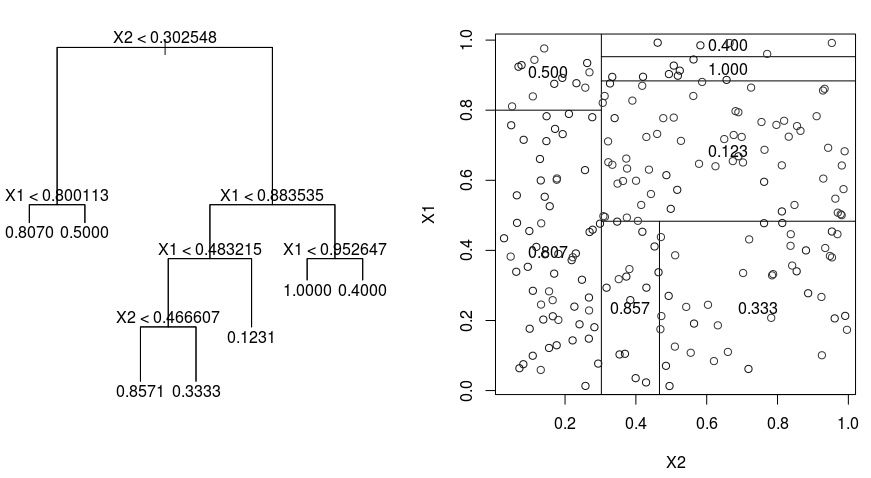
\includegraphics[width=\textwidth]{images/regr_tree}
    \caption[A regression tree and the induced tesselation of the input space]{A regression tree trained on a 2D dataset (left), and the induced tesselation of the input space (right). Taken from \cite{regr_tree_img}}
    \label{fig:regr_tree}
\end{figure}

Although many different regression tree learning algorithms exist, most of them follow the same approach, known as recursive binary splitting. This approach is:
\begin{itemize}
    \item top-down: the tree is built recursively starting from the root and going down to the leaves
    \item greedy: at each recursive step the local best split is performed, rather than a locally suboptimal one which might lead to the globally optimal tree
\end{itemize}

Different learning algorithms use different metrics for defining the "best" predictor on which to split the training samples, and the associated test to perform on it. These metrics generally measure the "homogeneity" of the target variable within a set of samples. One of the most commonly used is variance reduction \cite{variance_reduction}. The variance reduction of a node is defined as the total reduction of the variance of the target variable $y$ due to the split at this node; the predictor on which to split is the one which would cause the largest variance reduction.

This training process would continue to expand nodes by minimizing the chosen metric, until all leaves are homogeneous (i.e. all the training samples in the input space box associated to each leaf have the same response variable). Clearly, this may lead to overfitting the training data. To prevent it, we may decide to build the tree until a stopping criterion is reached: for example, we could fix the maximum depth of the tree as a hyperparameter of the learning algorithm (\texttt{max\_depth} in scikit-learn \cite{sklearn_random_forest}).

\smallskip

Regression trees are simple, highly interpretable and can be displayed graphically. However, they typically can't compete with other well-known regression approaches in terms of prediction performances. To reduce variance, prevent overfitting and hence increase performances, we may train a random forest, an ensemble learning technique that consists in growing multiple regression trees and then combining them to produce a prediction based on averaging the predictions given by each tree. It is based on two statistical techniques:
\begin{itemize}
    \item Bagging (bootstrap aggregating) \cite{bagging}: train an ensemble of $B$ models on $B$ different training sets, each obtained by randomly sampling $N$ instances with replacement from the original training set of $N$ samples; used to reduce the variance of a learning algorithm
    \item Feature bagging (random subspace method) \cite{feature_bagging}: at each split, the features on which to split are selected within a random subset of only $M'<M$ of the total set of $M$ predictors (a typical choice is $M'=\sqrt{M}$); used to reduce the correlation between regression trees in an ensemble
\end{itemize}

Combining many trees usually results in dramatic improvements in performances, at the expense of some loss of interpretability. An example of a random forest is reported in fig. \ref{fig:random_forest}.

\begin{figure}[hbt!]
    \centering
    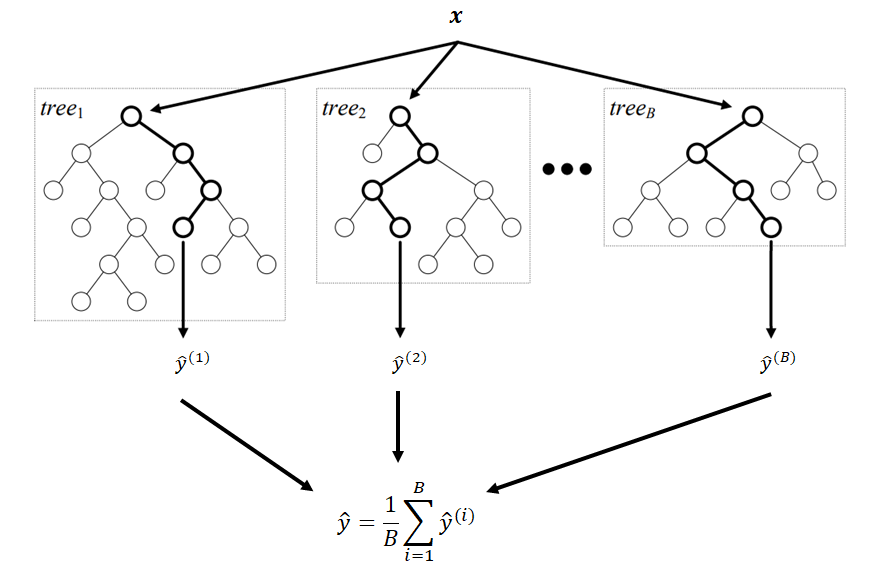
\includegraphics[width=\textwidth]{images/random_forest}
    \caption[A RF with $B$ regression trees]{A random forest regression model with $B$ regression trees. Adapted from \cite{random_forest_img}}
    \label{fig:random_forest}
\end{figure}





\subsection{Feed-forward neural network}
\label{sec:neural_network}
A \textbf{feed-forward neural network} (or simply neural network) is a non-linear model which can be used for regression tasks. The central idea is to extract linear combinations of the input variables as derived features, and then model the target as a nonlinear function of these features.

The "building block" of a neural network is the neuron, shown in fig. \ref{fig:neuron}

\begin{figure}
    \centering
    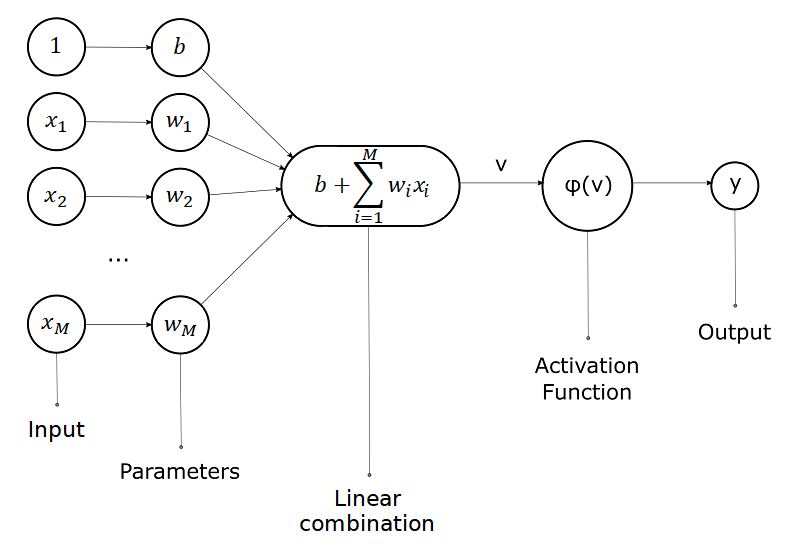
\includegraphics[width=0.9\textwidth]{images/neuron}
    \caption[A neuron in a NN]{A neuron in a neural network.}
    \label{fig:neuron}
\end{figure}

Inside a neuron, the linear combination of an input vector $\mathbf{x}$ with weights $w_1,\dots,w_M$ and bias $b$ is computed, which is then used as the argument of a so-called activation function. The activation function is a non-linear function used to make the neuron a non-linear model.

Neural networks are modeled as collections of neurons that are connected in a directed acyclic graph (DAG). In other words, the outputs of some neurons can become inputs to other neurons. The neurons of a neural network are organized into distinct layers of neurons, called fully-connected (FC) layers: each neuron of layer $i$ is connected to all the neurons of layer $i+1$. The FC layers between the input layer and the output layer are called hidden layers. The neurons of an output layer typically have the identity function as activation function. An example of a neural network architecture is depicted in fig. \ref{fig:neural_network}.

\begin{figure}[hbt!]
    \centering
    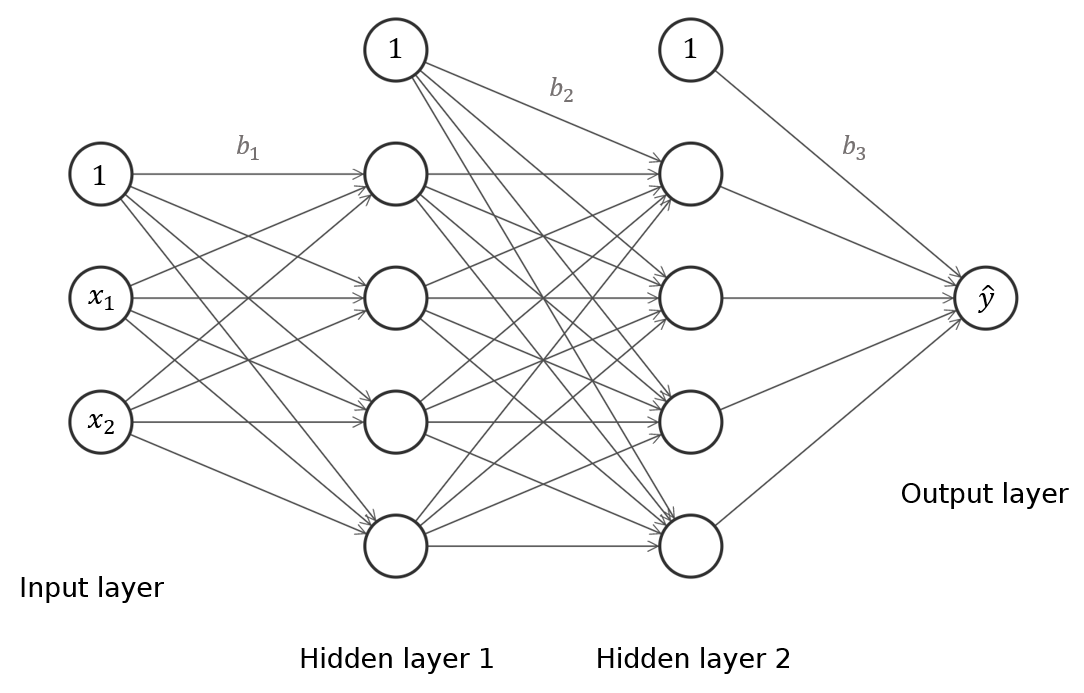
\includegraphics[width=\textwidth]{images/neural_network}
    \caption[A NN with 2 hidden layers]{A feed-forward neural network with a 2D input and 2 hidden layers with 4 neurons each.}
    \label{fig:neural_network}
\end{figure}

Each hidden layer extracts multiple hidden features from the input. Use of multiple hidden layers allows construction of hierarchical features at different levels of resolution \cite{hastie}.

The number of layers $L$ in a neural network, the number of neurons $N_1,\dots,N_L$ in each layer and the activation function $\phi$ for each neuron are hyperparameters to be optimized via e.g. grid search cross-validation (sec. \ref{sec:cv}), random search or simply by trial and error. The complexity of a neural network is measured by the number of its free parameters (weights and biases), which in turn depends by $L$ and $N_1,\dots,N_L$.

Due to neurons being non-linear models (thanks to the non-linear activation function), the neural network too is a non-linear model.
More complex neural networks are more expensive to train and to perform predictions with, but they have a higher representational power (i.e. they can learn functions which are more non-linear). On the other hand, neural networks which are too complex may overfit the training set, but this issue can be solved with proper regularization of the weights (as discussed in the next section).

\subsubsection{Training}
\label{sec:training_nn}
Training a neural network means estimating its weights and biases (collectively called "learnable parameters", $\bm{\theta}$) in such a way that the predicted values for the target variable associated to the training samples $\mathbf{x}_{1},\dots,\mathbf{x}_{N}$ are close to the ground-truth targets $y_1,\dots,y_N$. More specifically, we seek to find $\mathbf{w}^{(1)} \in \mathbb{R}^{N_1},\dots,\mathbf{w}^{(L)} \in \mathbb{R}^{N_L}$ and $\mathbf{b} \in \mathbb{R}^L$ such that the L2-regularized mean squared error (MSE) cost function
\begin{equation}
\text{MSE}_\text{L2}(\bm{\theta};X,\lambda) = \frac{1}{N} \sum_{i=1}^N(y_i-f(\mathbf{x}_{i};\bm{\theta}))^2 + \frac{1}{2}\lambda \sum_{w\in \bm{\theta} \setminus \mathbf{b}} w^2
\end{equation}
is minimized. The penalty factor $\lambda$ (also called \textit{weight decay} in the context of neural networks) measures how strongly large weights\footnote{Regularization is not applied to biases, for the same reason discussed in sec. \ref{sec:ridge} for ridge regression.} are to be penalized. Choosing $\lambda$ carefully is crucial to prevent overfitting the training set, as evident in fig. \ref{fig:lambda_nn}.

\begin{figure}[hbt!]
    \centering
    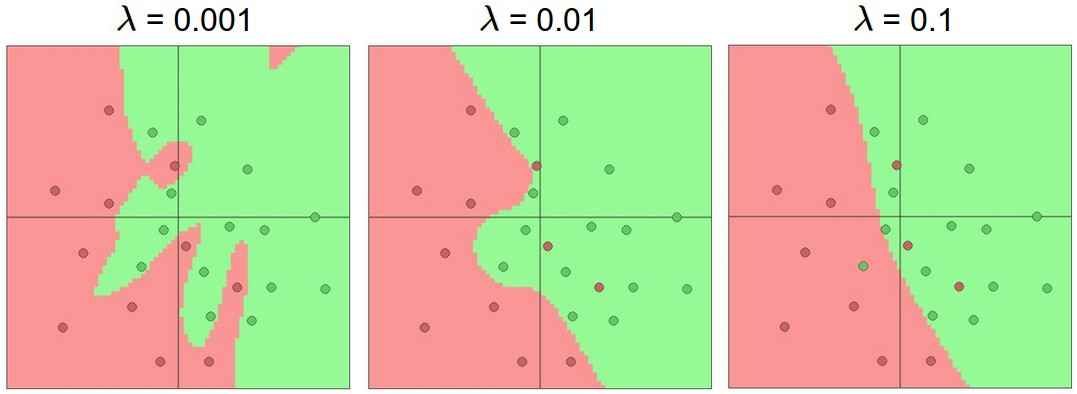
\includegraphics[width=0.9\textwidth]{images/lambda_nn}
    \caption[Decision boundaries of a NN for classification]{Decision boundaries of a neural network trained on a 2D dataset for a classification task, for varying values of $\lambda$. Taken from \cite{cs231n:nn1}}
    \label{fig:lambda_nn}
\end{figure}

As $f$ is a highly non-linear function in general, a closed form solution for the neural network learning problem is too impractical; rather, the problem is usually solved iteratively via SGD (sec. \ref{sec:sgd}).

SGD requires the gradient of the cost function $\mathcal{L}=\text{MSE}_{L2}$ with respect to each learnable parameter ($\nabla_{\bm{\theta}} \mathcal{L}$) to perform an update. Due to the particular topology of a feed-forward neural network, there exists a very efficient way of computing $\nabla_{\bm{\theta}} \mathcal{L}$ analytically, called \textbf{backpropagation} \cite{backprop}. Backpropagation computes each $\partial \mathcal{L}/\partial \theta$ through recursive application of the chain rule; its name suggests the idea that the prediction error is "propagated back" to the parameters "causing" it, and each $\partial \mathcal{L}/\partial \theta$ quantifies how much $\theta$ contributes to the error, thus how steeply we can update the parameter $\theta$ in order to minimize the error.

The depth of the neural network as well as the activation function must be chosen carefully, to avoid the vanishing gradient problem \cite{vanishing_gradient}. In particular, the network should be not too deep, otherwise the gradient of the cost function with respect to early layers' parameters would likely get small (because of a long chain of products between many quantities smaller than 1) and they would be updated very slowly (the neural network would not "learn" anymore). Moreover, the activation function should not operate in regions where it has a derivative approaching zero, as this would effectively kill the gradients of the parameters preceding that activation function. A very popular choice for the activation function is the Rectified Linear Unit (ReLU) \cite{relu}, $\phi(x) = \max(0,x)$, represented in fig. \ref{fig:relu}. ReLU has the advantage of being scale-invariant $(\max(0,ax)=a(\max(0,x))$, cheap to compute (only a comparison between $0$ and $x$ is needed) and non-saturating for $x>0$, which mitigates the vanishing gradient problem. On top of that, ReLU seems to work very well in practice \cite{relu_and_initialization}.

\begin{figure}[hbt!]
    \centering
    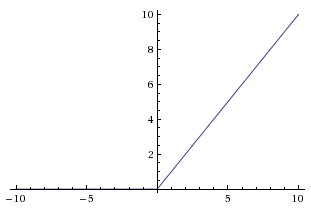
\includegraphics[width=0.6\textwidth]{images/relu}
    \caption[ReLU function]{ReLU function. Taken from \cite{cs231n:nn1}}
    \label{fig:relu}
\end{figure}

When training a neural network, it is common sense to standardize the data, as the scale of the training data has a relevant effect on the scale of the learned parameters and thus on the quality of the final solution. Having input variables scaled to zero mean and unit standard deviation implies that each feature will be deemed equally relevant in the learning process, and it can be shown that this improves the rate of convergence of training a neural network \cite{nn_standardization}.

Lastly, also the particular initialization of the parameters affects the rate of convergence of training. In particular, the cost function $\text{MSE}_\text{L2}$ is nonconvex and typically exhibits many local minima; as a result the estimates of the parameters are very sensible to their initialization. The recommended heuristic for initializing weights when using ReLU activation functions is Kaiming-He initialization \cite{relu_and_initialization}, which consists in drawing the initial value of each weight $w$ randomly according to a normal distribution
\[
w \sim \mathcal{N}\left(0,\frac{2}{n}\right)
\]
where $n$ is the number of inputs to a specific neuron (i.e. $n = |\mathbf{w_{l-1}}|$ where $l$ is the layer in which the neuron is located); biases, instead, are initialized to 0.
It can be proved that Kaiming-He initialization ensures that all neurons in the network initially have approximately the same output distribution with variance 1 and empirically improves the rate of convergence of the training process.





\section{Performance metrics for regression}
\label{sec:metrics}
To evaluate the performances of a regression model $f$, many different performance metrics can be used \cite{metrics}. These metrics generally measure how good (or bad) $f$ is at estimating the ground-truth target $y$ of a sample, i.e. how close (far) are the predictions $f(\mathbf{x}_{i};\bm{\theta}) = \hat{y}_i$ from $y_i$.
\begin{itemize}
    \item Mean squared error (MSE)
    \[
    \text{MSE} = \frac{1}{N} \sum_{i=1}^N (\hat{y}_i-y_i)^2
    \]
    It gives information on the prediction error that is committed on average. However, due to squaring, this metric does not have the same unit of measurement as the quantity that is being predicted; therefore, other metrics such as the RMSE or the MAE are usually preferred.
    \item Sum of squared errors (SSE)
    \[
    \text{SSE} = \sum_{i=1}^N (\hat{y}_i-y_i)^2
    \]
    Similar to the MSE but with a sum instead of an average operation.
    \item Root mean squared error (RMSE)
    \[
    \text{RMSE} = \sqrt{\frac{1}{N} \sum_{i=1}^N (\hat{y}_i-y_i)^2}
    \]
    It is similar to the MSE, but has the same unit of measurement as the target variable; however, it has no straightforward interpretation.
    \item Mean absolute error (MAE)
    \[
    \text{MAE} = \frac{1}{N} \sum_{i=1}^N |\hat{y}_i-y_i|
    \]
    It measures the average absolute difference between the predicted and real target values.
    \item Coefficient of determination ($R^2$)
    \[
    R^2 = 1 - \frac{\sum_{i=1}^N (y_i-\hat{y_i})^2}{\sum_{i=1}^N (y_i-\overline{y})^2}
    \]
    where $\overline{y}=\frac{1}{N}\sum_{i=1}^N y_i$.
    It provides a measure of how well the predictions $\hat{y}_i$ approximate the true values $y_i$. An $R^2$ of 1 indicates perfect prediction, whereas a model that always predicts the average value of y disregarding the input features ($f(\mathbf{x}_{i};\bm{\theta})=\overline{y}$) would get an $R^2$ of 0. The $R^2$ can also be negative, because the model can do arbitrarily worse than said constant model, in terms of MSE.
    The $R^2$ is not defined when $\overline{y}=y_1=\dots=y_N$; in this case, we set $R^2=1$ for perfect prediction and $R^2=0$ for imperfect prediction.
\end{itemize}





\section{\textit{K}-fold cross-validation}
\label{sec:cv}
To tune the hyperparameters which characterize a regression procedure\footnote{By "procedure" we refer in general to the whole training pipeline of a regression model, including data cleaning, data preprocessing and feature extraction steps. In fact, also these earlier steps can be characterized by user-defined hyperparameters, which are to be optimized.}, \textbf{(stratified) $K$-fold cross validation} can be used. It consists in randomly splitting the training set into $K$ subsets, called \textit{folds}. One fold is held out as a validation set, while the remaining $K-1$ folds are used for training the model: each prediction pipeline is fitted and trained on the $K-1$ training folds, and tested on the remaining validation fold, on which one or more performance metrics are evaluated (e.g. MSE or MAE). This procedure is repeated $K$ times, in order to use each fold as a validation set; therefore a total of $K$ regression models are trained. The resulting performance metrics are combined (e.g. averaged) over the $K$ rounds to give an estimate of the model's predictive performance on unseen data.

Typically, a grid search over different hyperparameters is performed through cross-validation. The hyperparameter combination achieving the highest cross-validation score is considered the optimal one, and the regression procedure with the optimal hyperparameters is refit on the whole training set, thus obtaining the final regression model. The cross-validation procedure is visually summarized in fig. \ref{fig:cross_validation}.

\begin{figure}[hbt!]
    \centering
    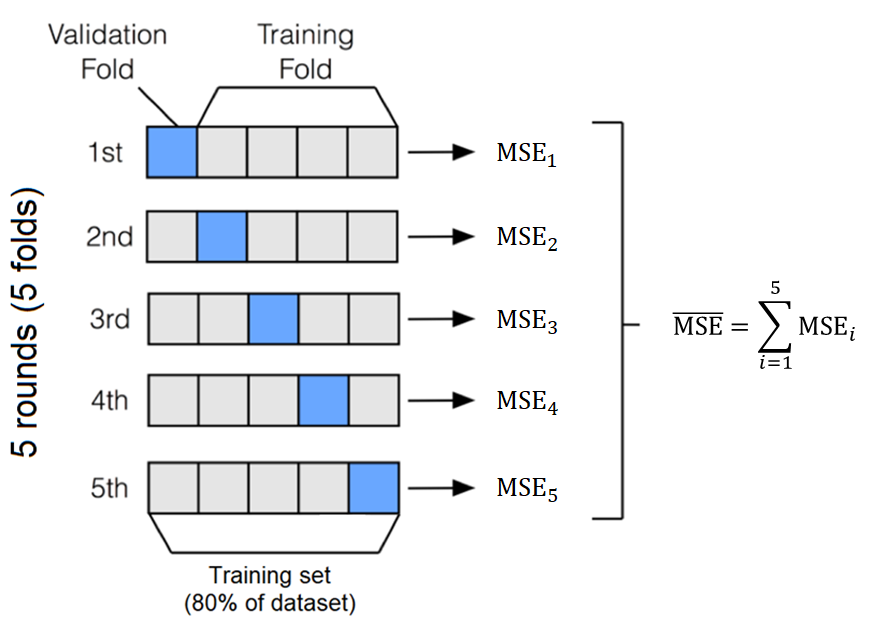
\includegraphics[width=0.9\textwidth]{images/cross_validation}
    \caption[5-fold cross-validation]{5-fold cross-validation procedure adopted in the experiments of this thesis (see sec. \ref{sec:regr_model_training}).}
    \label{fig:cross_validation}
\end{figure}

% simulink model + synthetic dataset generation
\chapter{EV model and synthetic dataset}
\label{sec:ev_model_ds_gen}

In order to train a machine learning regression model for estimating the SOH of an EV battery pack, it is critical to have a relatively large dataset of EV monitoring data to use for training. However, as of today, the availability of large-scale, freely accessible datasets of real EV monitoring data is very limited \cite{ev_no_real_datasets}.

To overcome this issue, we may generate the required dataset synthetically.

The first step is to develop a mathematical model of an electric vehicle (sec. \ref{sec:ev_model}). The model must fulfil the following requirements:
\begin{itemize}
    \item it should capture and mimic with high accuracy the mechanical dynamics of a real EV in driving conditions (speed, motor torque, braking force, etc.), as well as the electro-thermal dynamics of the vehicle's battery pack (current, voltage, SOC, temperature, etc.). % accuracy
    \item it should be flexible enough to mimic a wide variety of real EVs just by changing its main mechanical/electrical parameters (so as to match those of the desired EV model). % flexibility
    \item the user can simulate the model upon specifying a driving cycle, external temperature, initial battery temperature, initial battery SOC, battery age (SOH). % user interaction
    \item the computational cost of performing a simulation should be reasonably low. % computational cost
\end{itemize}

The model can be used after its definition (sec. \ref{sec:ev_model}) and parametrization (sec. \ref{sec:model_parametrization}) to simulate an EV in different driving conditions and then collect the physical signals generated by multiple simulations to build a synthetic dataset of EV monitoring data (sec. \ref{sec:ds_gen}).





\section{EV Simulink model}
\label{sec:ev_model}
A simple electric vehicle model fulfilling all the requirements has been built through MATLAB\textsuperscript\textregistered and Simulink\textsuperscript\textregistered programming environments.
Similarly to a real vehicle, it is composed of many mutually dependent subsystems (such as the electric motor, battery pack, wheels, brakes, and so on), connected to each other through signals that are calculated and updated at each time step of the simulation. A visual representation of the EV model is shown in fig. \ref{fig:ev_model} in appendix \ref{appendix}.

This design is heavily based on an existing model found on MATLAB File Exchange \cite{racing_lounge}, but many components have been modified and improved to better suit our experimental needs, most notably the battery pack and the braking subsystem. A brief technical description of each component of the model is given in this section. Variable names which are written with the \texttt{typewriter} font are user-defined parameters of the vehicle.



\subsection{Driver}
\label{sec:driver}
This subsystem implements a discrete-time proportional-integral (PI) controller to mimic a human driver for the vehicle. At each time step the controller tracks the input reference speed (e.g. driving cycle speed signal) and the current simulated vehicle speed, and tries to match them by acting on the brake and accelerator pedals. Brake pedal position (\textit{BPP}) and accelerator pedal position (\textit{APP}) take values in the range $[0,1]$, where 0 stands for "not pressed" and 1 for "fully pressed".



\subsection{Motor}
\label{sec:motor}
The electric traction motor is used for propelling the EV. It is powered by electricity (supplied by the battery pack) and generates the power to rotate the wheels of the vehicle. Many types of electric motors exist; the main distinction is between DC and AC motors, depending on the type of electric flow they require to operate. Nowadays, most EVs feature an AC motor \cite{renault_motors}, either asynchronous (high power output) or synchronous (high torque output). Such EVs feature a DC/AC inverter to convert the DC supplied by the battery pack to the AC required to operate the AC motor (fig. \ref{fig:ev_powertrain}).
\begin{figure}[htb]
    \centering
    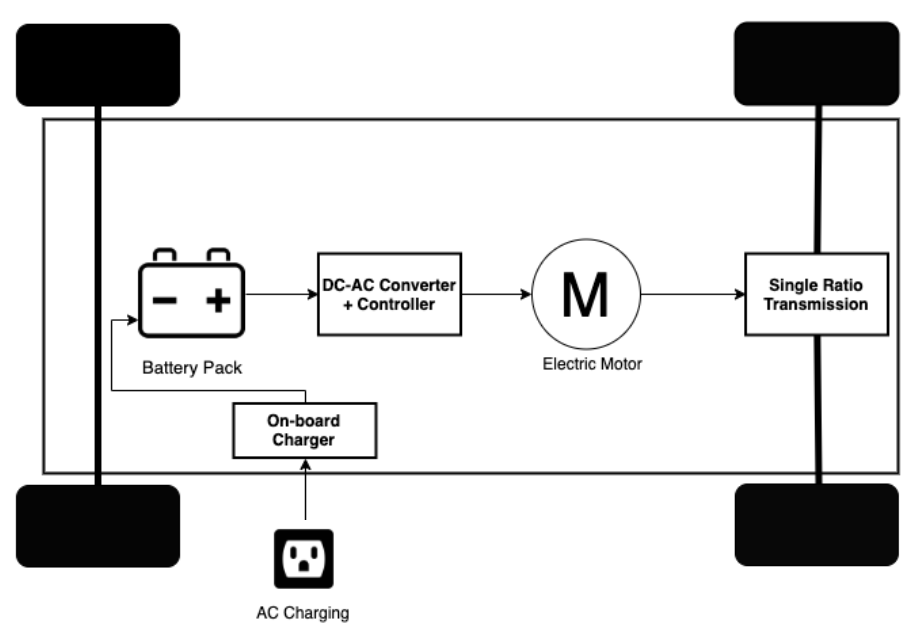
\includegraphics[width=0.7\textwidth]{images/ev_powertrain}
    \caption[Electrical powertrain of an EV]{Typical electrical powertrain of an EV equipped with an AC motor. Adapted from \cite{ev_reporter_powertrain}}
    \label{fig:ev_powertrain}
\end{figure}

Luckily, there exist a very simple characterization of an electric motor which is agnostic to its type and which is therefore used in our EV model \cite{hayes_ev_book}. Every electric motor can be characterized by two modes:
\begin{enumerate}
    \item Constant-torque mode: the motor can output a constant rated rotor torque, $T_{r(rated)}$, and the rotor power $P_r$ increases linearly with rotor/vehicle speed; achieved at low speeds.
    \item Constant-power mode: the motor can output a constant rated rotor power, $P_{r(rated)}$, and the rotor torque $T_r$ decreases inversely with rotor/vehicle speed; achieved at high speeds.
\end{enumerate}
This characterization is schematized in fig. \ref{fig:motor_characterization}.

\begin{figure}[htb]
    \centering
    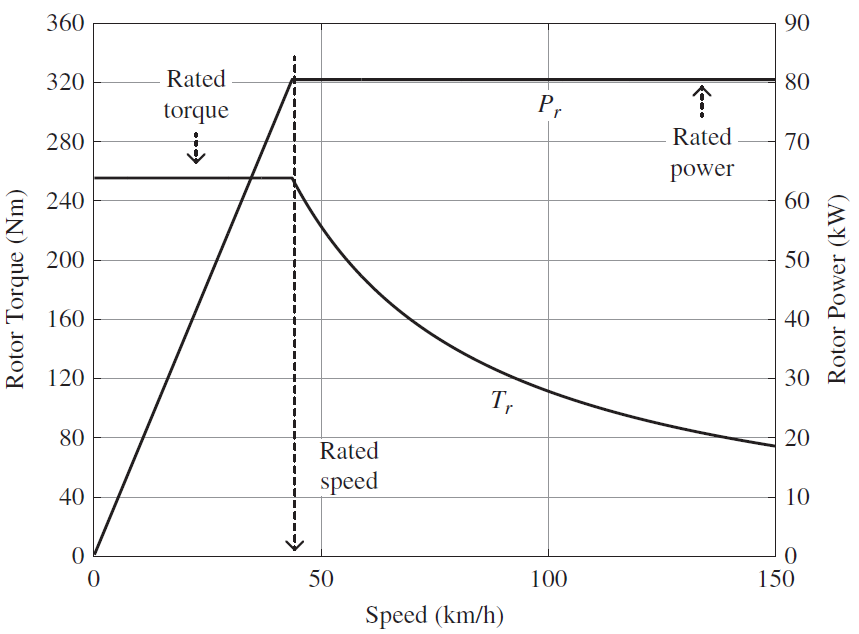
\includegraphics[width=0.7\textwidth]{images/motor_characterization}
    \caption[Torque-speed and power-speed envelopes]{Torque-speed and power-speed characterization curves for the electric motor of a 2015 Nissan Leaf. Taken from \cite{hayes_ev_book}}.
    \label{fig:motor_characterization}
\end{figure}

Moreover, there is a mathematical relation between power and torque
\begin{equation}
    P_r = T_r\omega_r = T_r \frac{v n_g}{r}
\end{equation}
where $\omega_r$ is the rotor speed [rad/s], $v$ is the vehicle speed [m/s], $n_g$ is the vehicle total drive ratio, $r$ is the radius of the wheels [m]. This means that we can characterize an electric motor just by specifying its torque-speed envelope.

On a final note, electric motors cannot convert 100\% of the electric power supplied by the battery ($P_{batt}$) to mechanical power, due to electrical and mechanical losses ($P_{losses}$) intrinsic to how the engine is designed. Losses are accounted for by introducing an efficiency term $\eta_{motor}$, so that the following equation holds:
\begin{equation}
P_r = P_{batt} - P_{losses} = \eta_{motor} P_{batt}
\end{equation}

We implement an electric motor in our EV model through the Mapped Motor block in Simulink \cite{mathworks:mapped_motor}. It is a mathematical model of an electric motor operated in torque-control mode. It can be parametrized by the user specifying a torque-speed envelope and other efficiency-related parameters:
\begin{itemize}
    \item \texttt{motorSpdRPM}: a vector of $N$ rotor speed values (in RPM), at which the value of maximum rotor torque is known
    \item \texttt{motorMaxTrq}: a vector of $N$ maximum rotor torque values [N$\cdot$m] which can be generated by the motor at a certain speed.
    \item \texttt{motorEff}: motor efficiency $\eta_{motor}$ at a rotor speed of \texttt{motorEffSpd} and a rotor torque of \texttt{motorEffTrq}
    \item \texttt{motorEffSpd}: rotor speed at which efficiency is measured [RPM]
    \item \texttt{motorEffTrq}: rotor torque at which efficiency is measured [N$\cdot$m]
    \item \texttt{motorPIron}: iron losses at the speed and torque at which efficiency is defined [W]
    \item \texttt{motorPBase}: fixed losses independent from torque and speed [W]
\end{itemize}

When the driver presses the accelerator pedal (i.e. $\text{APP}>0$), the model controls the mapped motor block with a rotor torque request of $\text{APP}\cdot T_{r(max)}(v)$. The block reads the current battery pack voltage $V_{batt}$, current rotor speed $\omega_r$ and the torque reference demand and computes the new rotor torque and the current $I_{batt}=P_{batt}/V_{batt}$ to be drawn from the battery to supply the needed power $P_r$.



\subsection{Braking system}
\label{sec:braking}
The braking system of an EV is based on two different contributes: friction braking and regenerative braking \cite{hayes_ev_book}.
The BPP value is interpreted as the fraction of the maximum total braking torque (\texttt{brqTrqMax}) that can be exerted on each wheel by the combination of friction and regenerative braking. The resulting braking torque "requested" by the driver is then distributed between the two braking subsystems, in such a way that the regenerative braking is used with priority and whenever possible, and friction braking only makes up for the remaining torque which cannot be supplied by regenerative braking. In formula:
\[
T_{braking} = \text{BPP} \cdot \text{\texttt{brqTrqMax}} = T_{regen} + T_{disc}
\]
The details about this distribution rule, known as brake blending \cite{brake_blending}, are discussed in the following paragraphs.

\paragraph{Regenerative braking}
Regenerative braking is a braking technology which achieves the aim of slowing down a vehicle while recharging its battery pack at the same time.
When the regenerative braking system is activated, the traction motor can develop a negative torque, up to the rated value in the forward direction. This torque reverses the usual flow of power such that the kinetic energy of the vehicle is converted to negative mechanical power on the driveshaft, and then converted to electrical power by the system. The generated electrical power is used to recharge the battery pack. This mechanism is schematized in fig. \ref{fig:regen_braking}.

\begin{figure}[htb]
    \centering
    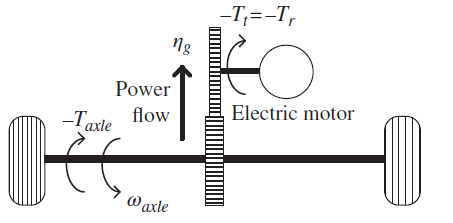
\includegraphics[width=0.6\textwidth]{images/regen_braking}
    \caption[Regenerative braking]{Regenerative braking scheme. Taken from \cite{hayes_ev_book}}.
    \label{fig:regen_braking}
\end{figure}

Recent studies \cite{regen_braking_limitations, wiki:regen_braking} suggest that regenerative braking is not energy-efficient nor sufficiently effective to apply at low speeds. For this reason, our model implements a user-defined cutoff speed (\texttt{RegenBrkSpd\_bpt}) above which the regenerative braking can be used. This is a common choice among different EV manufacturers. Fig. \ref{fig:braking_distribution} shows how braking torque is supplied by the two braking contributes at different speeds.

\begin{figure}[htb]
    \centering
    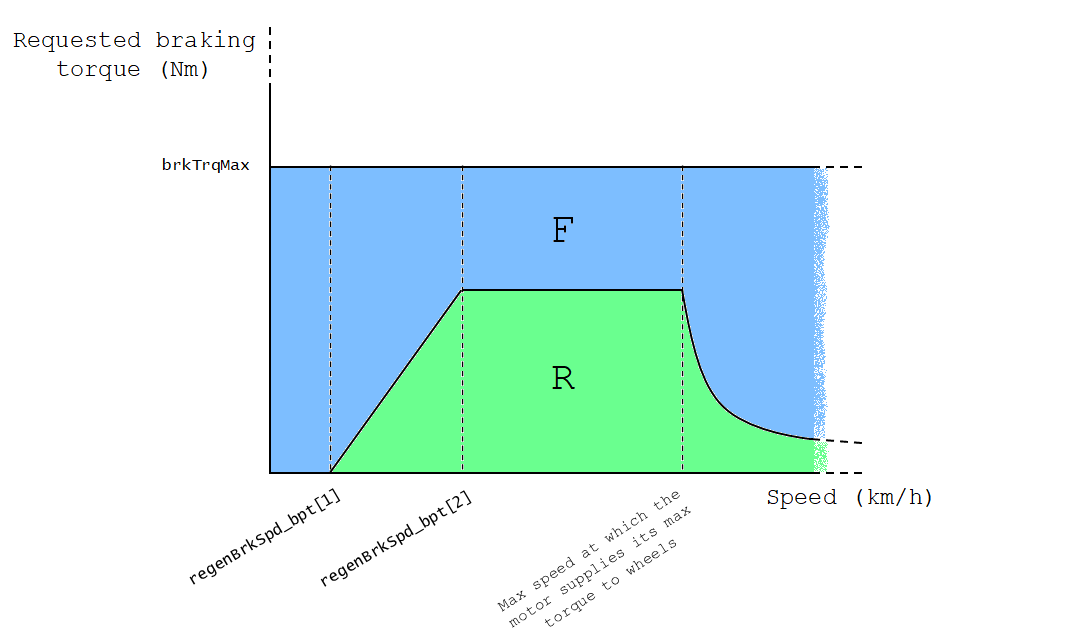
\includegraphics[width=\textwidth]{images/braking_distribution}
    \caption[Friction and regenerative braking torque distribution]{How the model distributes the requested braking torque between the regenerative (\texttt{R}) and friction (\texttt{F}) braking subsystems. Regenerative braking is activated when speed is above \texttt{RegenBrkSpd\_bpt[1]}. The maximum regenerative braking torque which can be supplied increases linearly with speed until a speed of \texttt{RegenBrkSpd\_bpt[2]} is reached. Above this speed, the regenerative brake is used to its full potential.}
    \label{fig:braking_distribution}
\end{figure}

The formula which models the maximum regenerative braking torque on each wheel given the speed $v$ of the vehicle is:
\begin{equation}
T_{regen} =
\begin{dcases}
    0 & \text{if } v \leq v_1\\
    \frac{v-v_1}{v_2-v_1} \cdot \frac{n_g T_{motor}(v)}{\eta_{regen}} & \text{if } v_1 < v \leq v_2\\
    \frac{n_g T_{motor}(v)}{\eta_{regen}} & \text{if } v > v_2\\
\end{dcases}
\end{equation}
where
\begin{itemize}
    \item $v_1$ (\texttt{RegBrkSpd\_bpt[1]}): cutoff speed above which the regenerative braking can be used [m/s]
    \item $v_2$ (\texttt{RegBrkSpd\_bpt[2]}): speed beyond which the regenerative brake can be used to its full potential [m/s]
    \item $n_g$ (\texttt{GR0*GRfinal}): overall gear ratio of the vehicle (see sec. \ref{sec:drivetrain})
    \item $T_{motor}(v)$ (previously written as $T_r(v)$ in sec. \ref{sec:motor}): maximum rotor torque at speed $v$ [N$\cdot$m]
    \item $\eta_{regen}$ (\texttt{regenEff}): efficiency factor for the regenerative braking
\end{itemize}
The negative torque $-T_{regen}/n_g$ is then used to control the motor (sec. \ref{sec:motor}), which will generate a negative current which recharges the battery pack.

\paragraph{Friction braking}
Friction braking is the conventional braking mechanism of all wheeled vehicles. A friction brake performs its function by pressing a brake pad against a rotating wheel. As a result, a friction force opposing the direction of the wheel is developed. In the process, the kinetic energy of the wheel is dissipated as heat.

Disc brakes (fig. \ref{fig:disc_brakes}) are the most commonly used form of friction brake for motor vehicles \cite{wiki:disc_brakes}. They are implemented in our EV model on all four wheels.

\begin{figure}[htb]
    \centering
    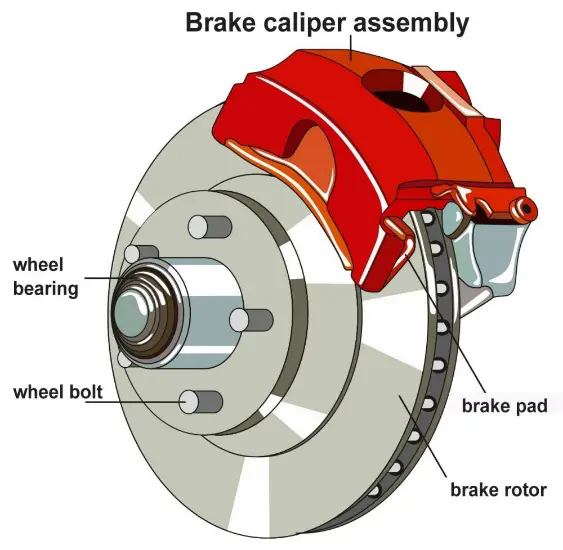
\includegraphics[width=0.45\textwidth]{images/disc_brakes}
    \caption[Disc brake]{Disc brake scheme. Taken from \cite{machinedesign_braking}}
    \label{fig:disc_brakes}
\end{figure}

The formula which models how much friction is generated on the wheel (measured as negative brake torque) is:
\begin{equation}
T_{disc} = \frac{\mu_{kinetic} P \pi d_{bore}^2 R_m N_{pads}}{4}
\label{eq:T_disc}
\end{equation}
where
\begin{itemize}
    \item $\mu_{kinetic}$ (\texttt{muKinetic}): coefficient of kinetic friction between disc pad and brake rotor
    \item $P$: total applied brake pressure [$\text{N}/\text{m}^2$]
    \item $d_{bore}$ (\texttt{discActBore}): brake actuator bore diameter [m]
    \item $R_m$ (\texttt{brakePadRadius}): mean radius of brake pad force application on the brake rotor [m]
    \item $N_{pads}$ (\texttt{numPads}): number of brake pads in the disc brake assembly
\end{itemize}
When the vehicle is still or the wheels are locked up (wheel skidding), the maximum friction braking torque on the wheel is still given by eq. \ref{eq:T_disc}, but $\mu_{static}$ (\texttt{muStatic}) is used in place of $\mu_{kinetic}$.

As anticipated, friction braking is used only when regenerative braking torque doesn't fulfil the braking torque request entirely: $T_{disc} = T_{braking} - T_{regen}$. The value $T_{disc}$ computed in this way is then used to compute the total pressure $P$ to be applied by the disc brakes to the wheels (sec. \ref{sec:wheels}), thanks to the inverse of eq. \ref{eq:T_disc}.



\subsection{Drivetrain}
\label{sec:drivetrain}
Drivetrain (also known as transmission, or driveline) is the set of rotating shafts and gears that distributes the mechanical power generated by the electric motor (sec. \ref{sec:motor}) to the wheels (sec. \ref{sec:wheels}).

While conventional internal combustion vehicles have a multi-gear gearbox with numerous ratios, nearly every electric car has a single-rate gearbox and no clutch, thus saving in cost, build complexity, weight and efficiency losses \cite{single_gear_ratio, ehsani_ev_book}. This is because electric motors have a much larger RPM range than the typical internal combustion engine (they often peak at about 20,000 RPM), they stay efficient across a very broad RPM range and produce a decent amount of torque at low RPM. EV designers pick a fixed gear ratio that provides a good compromise between acceleration and top speed \cite{single_gear_ratio}.

Gears are used across the drivetrain to reduce the angular velocity and increase torque before they are supplied to the wheels, while preserving power \cite{gear_trains}. A typical EV drivetrain is schematized in fig. \ref{fig:ev_drivetrain}. It consists of the gear between the motor and the driveshaft, the driveshaft, the differential (which houses the gear between the driveshaft and the drive axles), the two drive axles and the two drive wheels. Depending on the EV design, the drive wheels can be the rear or front ones (see sec. \ref{sec:wheels}); accordingly, the differential will be in the rear or front.

\begin{figure}[htb]
    \centering
    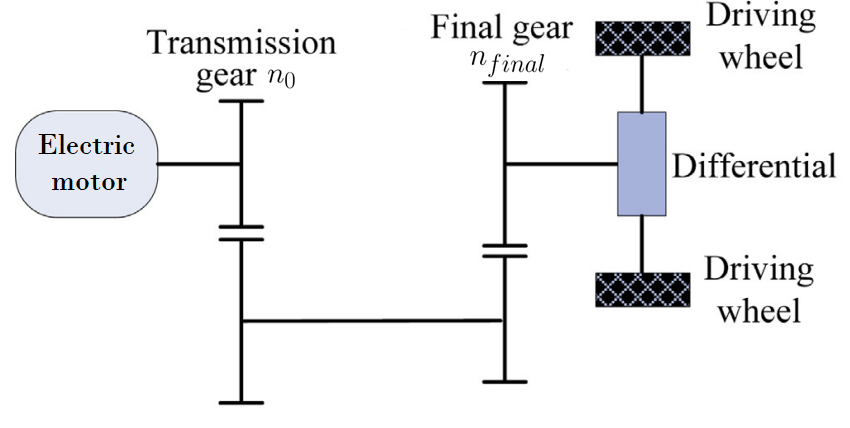
\includegraphics[width=0.7\textwidth]{images/ev_drivetrain}
    \caption[Drivetrain of an EV]{Schematic diagram of an EV drivetrain. Adapted from \cite{ev_drivetrain_schematic}}
    \label{fig:ev_drivetrain}
\end{figure}

The two gears have gear ratio $n_0$ and $n_{final}$, and efficiency of $\eta_0$ and $\eta_{final}$ (\texttt{GRfinal}) respectively; the driveshaft and drive axles have efficiency of $\eta_{ds}$ and $\eta_a$ respectively. It is convenient to express the overall gear ratio as
\begin{equation}
    n_g = n_0 \cdot n_{final}
\end{equation}
and the overall drivetrain efficiency as
\begin{equation}
    \eta_g = \eta_0 \cdot \eta_{ds} \cdot \eta_a \cdot \eta_{final}
\end{equation}

In the Simulink model, we simulate the components of the drivetrain with the following Simulink blocks:
\begin{itemize}
    \item First gear: Gearbox \cite{mathworks:gearbox}. Parameters: gear ratio $n_0$ (\texttt{GR0}), efficiency $\eta_0$ (\texttt{gearEff}).
    \item Driveshaft: Torsional Compliance \cite{mathworks:torsional_compliance}. Parameters: torsional stiffness $k_{ds}$ [N$\cdot$m/rad] (\texttt{driveshaft\_k}), damping $b_{ds}$ [N$\cdot$m$\cdot$s/rad] (\texttt{driveshaft\_b}), damping cutoff frequency $\omega_{ds}$ [rad/s] (\texttt{driveshaft\_wc}).
    \item Differential: Open Differential \cite{mathworks:differential}. Parameters: gear ratio $n_{final}$ (\texttt{GRfinal}), efficiency $\eta_{final}$ (\texttt{diffEff}).
    \item Drive axles: Torsional Compliance \cite{mathworks:torsional_compliance}. Parameters: torsional stiffness $k_a$ [N$\cdot$m/rad] (\texttt{axle\_k}), damping $b_a$ [N$\cdot$m$\cdot$s/rad] (\texttt{axle\_b}), damping cutoff frequency $\omega_a$ [rad/s] (\texttt{axle\_wc}).
\end{itemize}
Shaft efficiency can be computed from torsional stiffness, torsional damping and damping cutoff frequency\footnote{Note however that most EV manufacturers do not share such technical, low-level information about the vehicle components. For this reason, the user may want to stick with the default parameters taken from the model in \cite{racing_lounge}, which seem to work well in our experiments.}. The formula for computing it can be inferred from Simulink documentation \cite{mathworks:torsional_compliance}. 

If the vehicle is driven on a straight line, the torque at the differential is equally split between the left and right drive wheel. In this case, the torque that the drivetrain transmits from the motor to each drive wheel is computed as:
\begin{equation}
T_{wheel} = \frac{n_g \cdot \eta_{g} \cdot T_{motor}}{2}
\end{equation}
where
\begin{itemize}
    \item $n_g$: overall gear ratio
    \item $\eta_g$: total drivetrain efficiency
    \item $T_{motor}$: rotor torque [N$\cdot$m]
\end{itemize}



\subsection{Wheels}
\label{sec:wheels}
Wheels are modeled using the "Longitudinal wheel with disc brake" Simulink block \cite{mathworks:wheel}. The total longitudinal traction (or braking) force $F_x$ that the two drive wheels exert on the vehicle is given by Pacejka's Magic Formula \cite{magic_formula}:
\begin{equation}
F_x = F_z D \sin(C\arctan(B\kappa-E(B\kappa-\arctan(B\kappa))))
\end{equation}
where
\begin{itemize}
    \item $F_z$: vertical load on the tyre [N] (see sec. \ref{sec:body})
    \item $\kappa$: longitudinal wheel slip\footnote{Longitudinal wheel slip is defined as
    \[
    \kappa = -\frac{v-r_w\omega_w}{v}
    \]
    where $r_w$ and $\omega_w$ are respectively the wheel radius and wheel angular velocity, and $v$ is the longitudinal vehicle speed. When $\kappa=0$, the wheel is rolling without slipping; $\kappa>0$ means the wheel is slipping; $\kappa<0$ means the wheel is skidding.}
    \item $B, C, D, E$: stiffness, shape, peak and curvature factor
\end{itemize}
The four dimensionless coefficients are based on empirical data. We will assume that our EV model drives on dry tarmac, for which $B=10$, $C=1.9$, $D=1$, $E=0.97$ \cite{mathworks:wheel}. The block internally computes $\kappa$ knowing the wheel radius under load $r_w$ (\texttt{wheelRadius}), the vehicle speed $v$ and the torque that the drivetrain transfers to the wheel $T_{wheel}$ (sec. \ref{sec:drivetrain}).

This block also models the disc brake that operates on the wheel (sec. \ref{sec:braking}). When the disc brake is operated, $T_{wheel}$ is negative, therefore the computed $F_x$ is too (i.e. $F_x$ becomes a braking force).

Actually, tires are made of viscoelastic material, so they are subject to hysteresis energy loss, a phenomenon which results in rolling resistance \cite{rolling_resistance}. However, rolling resistance is not implemented in our model, as it would increase the complexity of the model and slow down the simulation. Nonetheless, one can take rolling resistance into account by using Pacejka's magic formula for rolling resistance (eq. 4.E70 of \cite{rolling_resistance}).
% https://www.youtube.com/watch?v=_S2lyaMgBQ8 see also first comment



\subsection{Vehicle body}
\label{sec:body}
The aerodynamic model of the vehicle body is implemented with the Vehicle Body 1DOF Longitudinal Simulink block \cite{mathworks:body}. It implements a one degree-of-freedom (1DOF) rigid vehicle body with constant mass undergoing longitudinal motion.

Assuming that the vehicle is driving on a flat road (angle of road grade $\gamma = 0$) with no wind, and that the two drive wheels are the front ones, this block internally solves the system of equations \ref{eq:free_body_system} associated to the vehicle's free body diagram (fig. \ref{fig:free_body_diagram}):
\begin{equation}
\begin{dcases}
    F_x = m\Ddot{x}\\
    F_x = F_{xF} + F_{xR} - F_{d,x}\\
    F_{d,x} = \frac{1}{2T_{air}R_{air}} C_d A_f P_{air} \dot{x}^2\\
    F_{zF} = \frac{bmg - h (F_{xF} + F_{xR})}{2(a+b)}\\
    F_{zR} = \frac{amg + h (F_{xF} + F_{xR})}{2(a+b)}\\
\end{dcases}
\label{eq:free_body_system}
\end{equation}

where
\begin{itemize}
    \item $F_x$: effective longitudinal force [N]
    \item $F_{xF}, F_{xR}$: total longitudinal force exerted by the two front (F) and rear (R) wheels [N]
    \item $F_{d,x}$: longitudinal aerodynamic drag force [N]
    \item $F_{zF}, F_{zR}$: normal load force on each front (F) and rear (R) wheel [N]
    \item $a$ (\texttt{a}): horizontal distance from vehicle's center of gravity (CG) to rear axle [m]
    \item $b$ (\texttt{b}): horizontal distance from vehicle's CG to front axle [m]
    \item $h$ (\texttt{h}): vehicle's CG height above axles [m]
    \item $m$ (\texttt{vehicleMass}): vehicle loaded mass [kg]
    \item $\Ddot{x}$: vehicle longitudinal acceleration [m/s\textsuperscript{2}]
    \item $A_f$ (\texttt{frontalArea}): vehicle's frontal area [m\textsuperscript{2}]
    \item $C_d$ (\texttt{dragCoeff}): frontal air drag coefficient
    \item $T_{air}, P_{air}, R_{air}$: air temperature [K], pressure [Pa] and specific gas constant [J$\cdot$kg\textsuperscript{-1}$\cdot$K\textsuperscript{-1}]
\end{itemize}

\begin{figure}[hbt!]
\centering
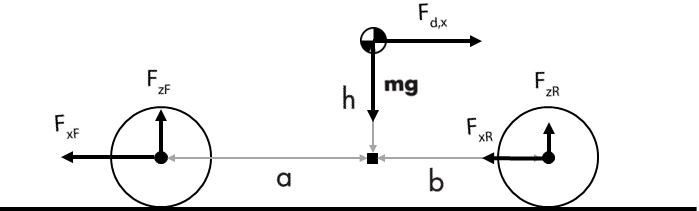
\includegraphics[width=0.8\textwidth]{images/free_body_diagram}
\caption[Free body diagram of a vehicle]{Free body diagram of the vehicle model. Adapted from \cite{mathworks:body}}
\label{fig:free_body_diagram}
\end{figure}

Given $F_{xF}$ and $F_{xR}$ (sec. \ref{sec:wheels}), the block outputs the vehicle speed $v$ and the normal load forces $F_{zF}$ and $F_{zR}$.



\subsection{Battery pack}
\label{sec:battery_pack}
The EV's battery pack is the most critical component of the model, since our aim is to predict its SOH. As discussed in sec. \ref{sec:li-ion}, an EV battery pack is actually a set of battery cells connected together in series and parallel; however, modeling an EV battery pack at the cell level would greatly increase the complexity of the simulation, and would be very hard to parametrize in a realistic way without extensive knowledge of the specific topology of the pack, its positioning inside the car and the specific features of the BMS in use. Therefore, we model our battery pack as if it consisted of only one high-voltage cell. To do so, our model uses the Generic Battery Model (GBM) block from the Simscape electrical Simulink library \cite{mathworks:battery}.
This block implements a generic dynamic equivalent circuit model (ECM) of a rechargeable battery, summarized in fig. \ref{fig:battery_ECM}.

\begin{figure}[htb]
    \centering
    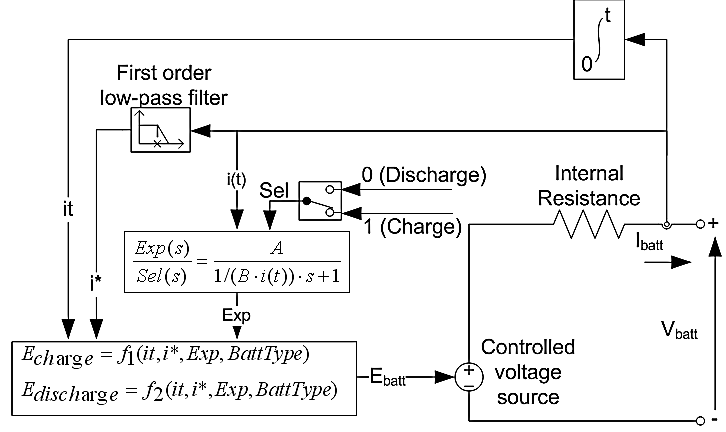
\includegraphics[width=0.8\textwidth]{images/battery_ECM.png}
    \caption[GBM internal ECM model]{Internal ECM model of the Generic Battery Model Simulink block. Taken from \cite{mathworks:battery}}
    \label{fig:battery_ECM}
\end{figure}

The GBM block interacts with the rest of the EV model as described in sec. \ref{sec:motor}: the motor reads the terminal voltage of the battery pack $V_{batt}$ and requests a current $I_{batt}$ based on the power demand $P_{batt}$. Then, a controlled current source imposes a current $I_{batt}$ to the battery pack, causing the terminal voltage to change accordingly to the charge/discharge characteristics specified for the battery pack (see "Discharge characteristics" paragraph). Moreover, the battery pack thermally interacts with the environment by reading the external temperature $T_a$, which can be set by the user. The equations which govern the electrical and thermal dynamics of the battery can be found in \cite{mathworks:battery}.

The GBM block parameters must be set according to those characterizing the battery pack of the specific EV we want to model. The parameters required to initialize the block are briefly discussed in the following paragraphs.

\subsubsection{Discharge characteristics}
\label{sec:discharge_characteristics}
In fig. \ref{fig:discharge_curve} a typical discharge curve of a battery cell is plotted. Three distinct sections can be observed:
\begin{enumerate}
    \item \textit{Exponential zone}: exponential voltage drop from a fully charged state $(V_{full},0)$ to a point $(V_{exp},Q_{exp})$;
    \item \textit{Nominal zone}: characterized by an almost constant voltage; from $(V_{exp},Q_{exp})$ to $(V_{nom},Q_{nom})$;
    \item \textit{Total discharge zone}: an extremely rapid voltage drop from $(V_{nom},Q_{nom})$ to $(V_{empty},Q_{full})$.
\end{enumerate}

\begin{figure}[htb]
    \centering
    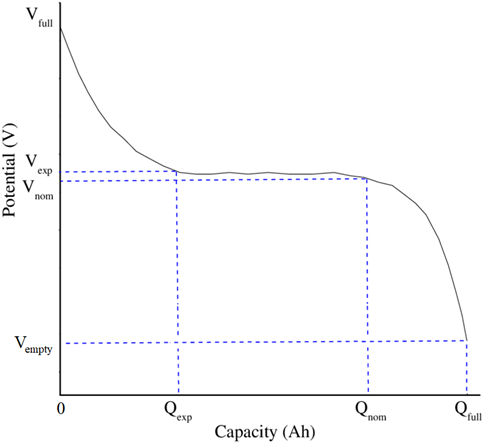
\includegraphics[width=0.7\textwidth]{images/discharge_curve.png}
    \caption[Discharge curve of a battery]{Typical discharge curve of a battery (at a certain C-rate, temperature, SOH), function of the discharged capacity $Q$. NB: the curve is not in scale, as the nominal zone is typically much wider compared to the exponential and total discharge zones.}
    \label{fig:discharge_curve}
\end{figure}

The discharge characteristics depend on a set of nominal conditions of operation defined by a nominal ambient temperature $T_{nom}$ (\texttt{Tnom1}) and a nominal discharge current $I_{nom}$ (\texttt{nomDischCurr}). To internally model the discharge curve in such operating conditions, the block requires the following parameters to be set:
\begin{itemize}
\item $Q_{rated}$ (\texttt{ratedCap}): rated capacity, i.e. the minimum effective capacity of the battery [Ah]
\item $R_{int}$ (\texttt{intRes}): internal resistance when the battery is fresh [$\Omega$]
\item $V_{full}$ (\texttt{fullychargV}): voltage at which the battery is fully charged [V]
\item $V_{exp}$ (\texttt{expV}): voltage at the end of the exponential zone [V]
\item $Q_{exp}$ (\texttt{expVCap}): discharged capacity at $V_{exp}$ [Ah]
\item $V_{nom}$ (\texttt{nomV}): voltage at the end of the nominal zone [V]
\item $Q_{nom}$ (\texttt{nomVCap}): discharged capacity at $V_{nom}$ [Ah]
\item $V_{empty}$ (\texttt{cutoffV}): voltage at which the battery is fully discharged [V]
\item $Q_{full}$ (\texttt{maxCap}): maximum theoretical capacity [Ah]
\end{itemize}

The user must also provide the SOC (\%) of the battery at the beginning of the simulation (\texttt{initSOC}). Finally, self-discharge is modeled by adding a large resistor of 2000 $\Omega$ in parallel with the battery terminals.

\subsubsection{Thermal model}
\label{sec:thermal_model}
The following parameters describe the discharge characteristics at a second operating condition (different from the nominal one), characterized by an external temperature $T_{nom,2}$ (\texttt{Tnom2}):
\begin{itemize}
\item $Q_{full,2}$ (\texttt{maxCap\_Tnom2}): maximum theoretical capacity [Ah]
\item $V_{full,2}$ (\texttt{initDischV\_Tnom2}): voltage at which the battery is fully charged [V]
\item $V_{90\%}$ (\texttt{V90maxCap\_Tnom2}): voltage when 90\% of $Q_{full,2}$ has been discharged [V]
\item $V_{exp,2}$ (\texttt{expV\_Tnom2}): voltage at the end of the exponential zone [V]
\item $Q_{exp,2}$ (\texttt{expVCap\_Tnom2}): discharged capacity at $V_{exp,2}$ [Ah]
\end{itemize}

Moreover, battery-to-ambient thermal interaction is described by two parameters: thermal resistance (\texttt{thRes}) and thermal time constant (\texttt{thTimeConst}). The user must also provide the internal temperature [°C] of the battery at the beginning of the simulation (\texttt{initBattTemp}), and the external temperature $T_a$ [°C], which can either be a constant or a time series of temperature measurements.

\subsubsection{Aging model}
\label{sec:aging_model}
Other than current and internal temperature, discharge characteristics are also affected by battery pack's SOH. The GBM block features a simple aging model of the battery, which is parametrized with the following parameters:
\begin{itemize}
    \item $Q_{EOL}$: maximum theoretical capacity at end of life [Ah]; usually for EV applications, battery pack's EOL is set at 80\% $Q_{full}$ (i.e. $0.8\times\text{\texttt{maxCap}}$) \cite{cap_eol}.
    \item $R_{EOL}$: internal resistance at end of life [$\Omega$]; set to $2\times\text{\texttt{intRes}}$ by default \cite{r_eol}.
    \item $I_c, I_{c,max}$ (\texttt{Ic, Icmax}): nominal and maximum charge current [A]
    \item $I_d, I_{d,max}$ (\texttt{Id, Idmax}): nominal and maximum discharge current [A]
    \item \texttt{cycLife\_100DOD\_Ic\_Id\_Ta1}: EFC at 100\% DOD, at $I_c$ and $I_d$, to reach EOL
    \item \texttt{cycLife\_25DOD\_Ic\_Id\_Ta1}: EFC at 25\% DOD, at $I_c$ and $I_d$, to reach EOL
    \item \texttt{cycLife\_100DOD\_Ic\_Idmax\_Ta1}: EFC at 100\% DOD, at $I_c$ and $I_{d,max}$, to reach EOL
    \item \texttt{cycLife\_100DOD\_Icmax\_Id\_Ta1}: EFC at 100\% DOD, at $I_{c,max}$ and $I_d$, to reach EOL
    \item $T_{amb,2}$ (\texttt{Ta2}): a second ambient temperature at which the aging model is parametrized [°C]
    \item \texttt{cycLife\_100DOD\_Ic\_Id\_Ta2}: EFC at 100\% DOD, at $I_c$ and $I_d$ and temperature $T_{amb,2}$, to reach EOL
\end{itemize}
The user must also specify the battery age (as number of EFC) which characterizes the battery pack throughout the simulation (\texttt{initBattAge}).

The mathematical relationship between the battery age expressed in number of EFC and the percentage of fresh maximum capacity (which is our reference definition of SOH, eq. \ref{eq:soh}) is not linear in general \cite{efc_vs_soh}. However, a simple simulation of a battery characterization test may be performed to unambiguously associate an EFC level to the correspondent SOH value (sec. \ref{sec:efc2soh}).



\subsection{Known limitations}
\label{sec:known_limitations}
Our proposed EV model suffers from several limitations, mainly due to its low-complexity design. Known limitations are:
\begin{itemize}
    \item Energy losses due to auxiliary devices (such as air-conditioner, power steering, car lights and so on), which are usually powered by a 12V auxiliary battery \cite{auxiliary_battery}, are not modeled.
    \item Rolling resistance is not modeled, as explained in sec. \ref{sec:wheels}.
    \item It is often difficult to retrieve technical specifications of a specific EV model from the Internet, as this information is not always publicly shared by EV manufacturers. Required specifications which could not be found have been estimated indirectly by exploiting real EV field data or otherwise made up by choosing plausible values.
    \item Many EVs can operate in different driving modes, with the aim of adapting the energy consumption to a desired driving profile, ultimately optimizing the vehicle's driving range \cite{vw_driving_modes}. Due to the huge variety of driving modes implemented by different EV manufacturers, the model is designed with a default driving mode.
    \item A fair validation of the Simulink EV model by means of monitoring data acquired from real EVs is impossible, because an EV's BMS monitors only a fraction of the many different variables and factors which characterize driving. For instance: road type, slope, road curves, wind direction and speed are usually not recorded. For this reason, our model is designed to mimic the dynamics of a car moving in the forward direction on a flat dry tarmac road.
    \item The ECM model which characterizes Simulink generic battery block (sec. \ref{sec:battery_pack}) has several limitations and assumptions in its design, as stated in its documentation \cite{mathworks:battery}. For instance:
    \begin{itemize}
        \item internal resistance is assumed to be constant during charging and discharging and does not vary with the amplitude of the current;
        \item the capacity of the battery does not change with the amplitude of the current (there is no Peukert effect);
        \item the battery has no memory effect.
    \end{itemize}
    \item Simulink generic battery block implements a very low complexity thermal model, which cannot precisely capture heat transfer phenomena at the cell and module level and between the heat-producing components of the car (e.g. the motor) and the battery itself. Moreover, the thermal behaviour of the block seems to be independent of the SOH of the battery (as opposed to real batteries, as discussed in sec. \ref{sec:li-ion}). % However, this is not a big deal, because temperature doesn't affect SOH so much: https://onlinelibrary.wiley.com/doi/epdf/10.1002/er.6005
    \item The user cannot specify battery's SOH directly, but rather the battery age expressed in number of EFC; this limitation is overcome by mapping EFC levels to SOH values (see sec. \ref{sec:efc2soh}).
\end{itemize}





\section{EV model parametrization}
\label{sec:model_parametrization}
In order to generate a synthetic dataset of monitoring data, the EV Simulink model must be parametrized according to the technical specifications of a specific EV model. In this thesis, we focus on two EV models by Volkswagen: the e-up! (18.7 kWh) and the e-Golf (35.8 kWh). This choice is due to the availability of real driving session monitoring data for these two models (sec. \ref{sec:aviloo_ds}), acquired from a private EV fleet management company (sec. \ref{sec:aviloo}).

The required technical specifications for the VW e-up! and VW e-Golf are reported in table \ref{tab:eup_egolf_specs}. As mentioned in sec. \ref{sec:known_limitations}, retrieving the actual technical specifications for an EV model is not an easy task in general. For this reason, whenever any specification was not directly found on the Internet or in the literature it has been either:
\begin{itemize}
\item estimated with a parameter estimation procedure (see sec. \ref{sec:parameter_estimation}); marked with "\textbf{est}" in table \ref{tab:eup_egolf_specs}
\item computed indirectly from pertaining sources, assumed from sources pertaining to similar models, or otherwise left as Simulink's default value; marked with "\textbf{*}" in table \ref{tab:eup_egolf_specs}
\end{itemize}





\newgeometry{left=2.05cm,right=2.05cm,footskip=20mm}

\begin{table}[H]
\scriptsize
\centering
\captionsetup{size=small}
\caption[Technical specifications for the VW e-up! and the VW e-Golf]{Technical specifications for the VW e-up! (18.7 kWh) and the VW e-Golf (35.8 kWh). Parameters marked with 'est' are estimated through parameter estimation (sec. \ref{sec:parameter_estimation}), and those marked with '*' are computed indirectly from pertaining sources or left as default.}
\label{tab:eup_egolf_specs}
\begin{tabular}[t]{cllccccc}
\toprule
& \breakcellleft{Parameter\\name} & \breakcellleft{Workspace\\variable} & e-up! & e-Golf & Unit & \breakcell{Source\\(e-up!)} & \breakcell{Source\\(e-Golf)} \\
\midrule
\multirow{12}{*}{\STAB{\rotatebox[origin=c]{90}{Motor}}}
& Rotor speed breakpoints & \texttt{motorSpdRPM} & (see source) & (see source) & RPM & \cite{motorSpdRPM-eup} & \cite{motorSpdRPM-egolf}
\\[0.15cm]
& \breakcellleft{Max. motor torque at\\rotor speed breakpoints} & \texttt{motorMaxTrq} & (see source) & (see source) & N$\cdot$m & \cite{motorSpdRPM-eup} & \cite{motorSpdRPM-egolf}
\\[0.28cm]
& Motor efficiency & \texttt{motorEff} & 0.95 & 0.95 & -- & \cite{motorEff1,motorEff2},* & \cite{motorEff1,motorEff2},*
\\[0.15cm]
& \breakcellleft{Rotor speed at which\\motor eff. is measured} & \texttt{motorEffSpd} & 6500 & 6500 & RPM & \cite{motorSpdRPM-eup,motorEff2},* & \cite{motorSpdRPM-egolf,motorEff2},*
\\[0.28cm]
& \breakcellleft{Rotor torque at which\\motor eff. is measured} & \texttt{motorEffTrq} & 89 & 146 & N$\cdot$m & \cite{motorSpdRPM-eup,motorEff2},* & \cite{motorSpdRPM-egolf,motorEff2},*
\\[0.28cm]
& Iron losses & \texttt{motorPIron} & 0 & 0 & W & * & *
\\[0.15cm]
& Fixed losses & \texttt{motorPBase} & 0 & 0 & W & * & *
\\[0.15cm]
\midrule
\multirow{13}{*}{\STAB{\rotatebox[origin=c]{90}{Braking system}}}
& \breakcellleft{Max. total braking\\torque} & \texttt{brqTrqMax} & 2000 & 2000 & N$\cdot$m & \cite{brkTrqMax},* & \cite{brkTrqMax},*
\\[0.28cm]
& \breakcellleft{Regen. braking cutoff\\speeds} & \texttt{RegenBrkSpd\_bpt} & [18, 32.4] & [18, 32.4] & km/h & \cite{racing_lounge},* & \cite{racing_lounge},*
\\[0.28cm]
& Regen. efficiency factor & \texttt{regenEff} & 0.75 & 0.75 & -- & \cite{racing_lounge},* & \cite{racing_lounge},*
\\[0.15cm]
& Kinetic friction coeff. & \texttt{muKinetic} & 0.35 & 0.35 & -- & \cite{racing_lounge},* & \cite{racing_lounge},*
\\[0.15cm]
& Static friction coeff. & \texttt{muKinetic} & 0.9 & 0.9 & -- & \cite{racing_lounge},* & \cite{racing_lounge},*
\\[0.15cm]
& \breakcellleft{Brake actuator bore\\diameter} & \texttt{discActBore} & 0.05 & 0.05 & m & \cite{racing_lounge},* & \cite{racing_lounge},*
\\[0.28cm]
& Brake pad radius & \texttt{brakePadRadius} & 0.15 & 0.15 & m & \cite{racing_lounge},* & \cite{racing_lounge},*
\\[0.15cm]
& N. of brake pads & \texttt{numPads} & 2 & 2 & -- & \cite{racing_lounge},* & \cite{racing_lounge},*
\\[0.15cm]
\midrule
\multirow{16}{*}{\STAB{\rotatebox[origin=c]{90}{Drivetrain}}}
& First gear ratio & \texttt{GR0} & 1.576 & 2.7 & -- & \cite{eup_tech_specs1} & \cite{egolf_tech_specs1}
\\[0.15cm]
& First gear efficiency & \texttt{gearEff} & 0.95 & 0.95 & -- & \cite{gearEff},* & \cite{gearEff},*
\\[0.15cm]
& Driveshaft tors. stiffness & \texttt{driveshaft\_k} & 2500 & 2500 & N$\cdot$m/rad & \cite{racing_lounge},* & \cite{racing_lounge},*
\\[0.15cm]
& Driveshaft tors. damping & \texttt{driveshaft\_b} & 10 & 10 & N$\cdot$m$\cdot$s/rad & \cite{racing_lounge},* & \cite{racing_lounge},*
\\[0.15cm]
& \breakcellleft{Driveshaft damping\\cutoff frequency} & \texttt{driveshaft\_wc} & 500 & 500 & rad/s & \cite{racing_lounge},* & \cite{racing_lounge},*
\\[0.28cm]
& Final gear ratio & \texttt{GRfinal} & 5.176 & 3.61 & -- & \cite{eup_tech_specs1} & \cite{egolf_tech_specs1}
\\[0.15cm]
& Differential efficiency & \texttt{diffEff} & 0.95 & 0.95 & -- & \cite{gearEff},* & \cite{gearEff},*
\\[0.15cm]
& Axle tors. stiffness & \texttt{axle\_k} & 5000 & 5000 & N$\cdot$m/rad & \cite{racing_lounge},* & \cite{racing_lounge},*
\\[0.15cm]
& Axle tors. damping & \texttt{axle\_b} & 10 & 10 & N$\cdot$m$\cdot$s/rad & \cite{racing_lounge},* & \cite{racing_lounge},*
\\[0.15cm]
& \breakcellleft{Axle damping\\cutoff frequency} & \texttt{axle\_wc} & 400 & 400 & rad/s & \cite{racing_lounge},* & \cite{racing_lounge},*
\\[0.28cm]
\midrule
\multirow{10}{*}{\STAB{\rotatebox[origin=c]{90}{Body and wheels}}}
& Wheel radius & \texttt{wheelRadius} & 0.293 & 0.316 & m & \cite{eup_tech_specs1,wheelRadius_calc} & \cite{egolf_tech_specs1,wheelRadius_calc}
\\[0.15cm]
& CG to front axle & \texttt{a} & 1.04 & 1.21 & m & \cite{eup_tech_specs3,eup_tech_specs4,CG_calc} & \cite{egolf_tech_specs1,egolf_tech_specs2,CG_calc}
\\[0.15cm]
& CG to rear axle & \texttt{b} & 1.38 & 1.42 & m & \cite{eup_tech_specs3,eup_tech_specs4,CG_calc} & \cite{egolf_tech_specs1,egolf_tech_specs2,CG_calc}
\\[0.15cm]
& CG height above axles & \texttt{h} & 0.35 & 0.35 & m & \cite{racing_lounge},* & \cite{racing_lounge},*
\\[0.15cm]
& Vehicle mass & \texttt{vehicleMass} & 1375 & 1690 & kg & \cite{eup_tech_specs2} & \cite{egolf_tech_specs1}
\\[0.15cm]
& Frontal area & \texttt{frontalArea} & 2.07 & 2.21 & m\textsuperscript{2} & \cite{eup_tech_specs3},* & \cite{egolf_tech_specs3},*
\\[0.15cm]
& Air drag coefficient & \texttt{dragCoeff} & 0.32 & 0.27 & -- & \cite{eup_tech_specs2} & \cite{egolf_tech_specs1}
\\[0.15cm]
\midrule
\multicolumn{8}{r}{continued on next page}\\
%\bottomrule
\end{tabular}
\end{table}

\begin{table}[H]
\scriptsize
\centering
\captionsetup{justification=centering,size=small}
\caption*{\textbf{Table \ref{tab:eup_egolf_specs}} (continued)}
\begin{tabular}[t]{cllccccc}
\multicolumn{8}{l}{continued from previous page}\\[0.15cm]
\toprule
& \breakcellleft{Parameter\\name} & \breakcellleft{Workspace\\variable} & e-up! & e-Golf & Unit & \breakcell{Source\\(e-up!)} & \breakcell{Source\\(e-Golf)} \\
\midrule
\multirow{17}{*}{\STAB{\rotatebox[origin=c]{90}{Battery pack - discharge}}}
& Nom. amb. temperature & \texttt{Tnom1} & 20 & 20 & °C & \cite{mathworks:battery} & \cite{mathworks:battery}
\\[0.15cm]
& Nom. disch. current & \texttt{nomDischCurr} & 24.8 & 54.2 & A & est & est
\\[0.15cm]
& Rated capacity & \texttt{ratedCap} & 50.3 & 116.1 & Ah & \cite{eup_tech_specs2}, est & \cite{egolf_tech_specs1}, est
\\[0.15cm]
& Internal resistance & \texttt{intRes} & 0.08 & 0.075 & $\Omega$ & \cite{intRes}, est & \cite{intRes}, est
\\[0.15cm]
& Voltage at 100\% SOC & \texttt{fullychargV} & 429.9 & 386.6 & V & \cite{eup_tech_specs5}, est & \cite{intRes}, est
\\[0.15cm]
& \breakcellleft{Voltage at the end of\\the exp. zone ($V_{exp}$)} & \texttt{expV} & 407.6 & 351.9 & V & est & est
\\[0.28cm]
& Capacity disch. at $V_{exp}$ & \texttt{expVCap} & 5.0 & 10.6 & Ah & est & est
\\[0.15cm]
& \breakcellleft{Voltage at the end of\\the nom. zone ($V_{nom}$)} & \texttt{nomV} & 345.6 & 304.3 & V & \cite{eup_tech_specs2}, est & \cite{egolf_tech_specs1}, est
\\[0.15cm]
& Capacity disch. at $V_{nom}$ & \texttt{expVCap} & 44.0 & 95.8 & Ah & est & est
\\[0.15cm]
& Voltage at 0\% SOC & \texttt{cutoffV} & 297.2 & 288.7 & V & \cite{eup_tech_specs5}, est & \cite{intRes}, est
\\[0.15cm]
& Max. theor. capacity & \texttt{maxCap} & 49.9 & 107.7 & Ah & est & est
\\[0.15cm]
\cmidrule{2-8}
\multirow{17}{*}{\STAB{\rotatebox[origin=c]{90}{Battery pack - thermal}}}
& \breakcellleft{2nd nom. amb.\\temperature ($T_{nom,2}$)} & \texttt{Tnom2} & -30 & -30 & °C & \cite{mathworks:battery} & \cite{mathworks:battery}
\\[0.28cm]
& \breakcellleft{Max. theor. capacity\\at $T_{nom,2}$} & \texttt{maxCap\_Tnom2} & 38.3 & 87.9 & Ah & est & est
\\[0.28cm]
& \breakcellleft{Voltage at 100\% SOC\\at $T_{nom,2}$} & \texttt{initDischV\_Tnom2} & 397.2 & 350.2 & V & est & est
\\[0.28cm]
& \breakcellleft{Voltage when 90\% disch.\\cap., at $T_{nom,2}$} & \texttt{V90maxCap\_Tnom2} & 304.5 & 289.8 & V & est & est
\\[0.28cm]
& \breakcellleft{Voltage at the end of\\the exp. zone, at\\$T_{nom,2}$ ($V_{exp,2}$)} & \texttt{expV\_Tnom2} & 392.2 & 326.9 & V & est & est
\\[0.45cm]
& \breakcellleft{Cap. discharged at\\$V_{exp,2}$, at $T_{nom,2}$} & \texttt{expVCap\_Tnom2} & 2.0 & 9.9 & Ah & est & est
\\[0.28cm]
& Thermal resistance & \texttt{thRes} & 0.065 & 0.013 & °C/W & est & est
\\[0.15cm]
& Thermal time constant & \texttt{thTimeConst} & 30000 & 27000 & s & est & est
\\[0.15cm]
\cmidrule{2-8}
\multirow{20}{*}{\STAB{\rotatebox[origin=c]{90}{Battery pack - aging}}}
& Nom. charge current & \texttt{Ic} & 7.5 & 7.5 & A & * & *
\\[0.15cm]
& Max. charge current & \texttt{Icmax} & 9.58 & 9.58 & A & * & *
\\[0.15cm]
& Nom. discharge current & \texttt{Id} & 17.83 & 17.83 & A & * & *
\\[0.15cm]
& Max. discharge current & \texttt{Idmax} & 75.93 & 75.93 & A & * & *
\\[0.15cm]
& \breakcellleft{EFC @ 100\% DOD,\\$I_c$, $I_d$ to EOL} & \texttt{cycLife\_100DOD\_Ic\_Id\_Ta1} & 3000 & 3000 & -- & \cite{battery_research},* & \cite{battery_research},*
\\[0.28cm]
& \breakcellleft{EFC @ 25\% DOD,\\$I_c$, $I_d$ to EOL} & \texttt{cycLife\_25DOD\_Ic\_Id\_Ta1} & 20000 & 20000 & -- & * & *
\\[0.28cm]
& \breakcellleft{EFC @ 100\% DOD,\\$I_c$, $I_{d,max}$ to EOL} & \texttt{cycLife\_100DOD\_Ic\_Idmax\_Ta1} & 2000 & 2000 & -- & \cite{battery_research},* & \cite{battery_research},*
\\[0.28cm]
& \breakcellleft{EFC @ 100\% DOD,\\$I_{c,max}$, $I_d$ to EOL} & \texttt{cycLife\_25DOD\_Icmax\_Id\_Ta1} & 2500 & 2500 & -- & \cite{battery_research},* & \cite{battery_research},*
\\[0.28cm]
& \breakcellleft{2nd amb. temperature\\($T_{amb,2}$)} & \texttt{Ta2} & 45 & 45 & °C & \cite{mathworks:battery} & \cite{mathworks:battery}
\\[0.28cm]
& \breakcellleft{EFC @ 100\% DOD,\\$I_c$, $I_d$, $T_{amb,2}$ to EOL} & \texttt{cycLife\_100DOD\_Ic\_Id\_Ta2} & 2500 & 2500 & -- & * & *
\\[0.28cm]
\bottomrule
\end{tabular}
\end{table}

\restoregeometry





\subsection{Parameter estimation}
\label{sec:parameter_estimation}
Most parameters specific to the battery pack have been estimated with Simulink Parameter Estimator app \cite{mathworks:parameter_estimator}. Parameter estimation can be formulated as a constrained or unconstrained optimization problem (sec. \ref{sec:opt_prob}).

The parameters estimated with this procedure are those marked with "est" in table \ref{tab:eup_egolf_specs}. We set up a parameter estimation experiment by picking a real driving session from each of the two acquired real datasets to use as experimental input and output data. The battery pack current signals from the two driving sessions have been extracted and set as the input signals for the simulation. We have chosen two battery test driving sessions, as they produce signals spanning from a full charge to an almost full discharge of the battery pack: these wide operating conditions ensure that the found parameters are well-fitted for almost any section of the discharge curve of the battery pack. The initial SOC, initial battery temperature and battery SOH of the simulated battery pack are set accordingly to the selected driving session. The battery pack voltages have been chosen as the measured output signals; parameters have been tuned so that the simulated voltage signal matches the experimental one as much as possible (i.e. the SSE over the measured signal time base\footnote{The measured signal time base consists of all the timestamps for which the measured signal is specified, whereas the simulated signal time base consists of all the timestamps for which the model is simulated. The two time bases are different in general. By default, Simulink Parameter Estimator computes the cost function only in the timestamps of the measured signal time base. Our Simulink model uses a variable-step discrete solver, which adjusts the simulation step size during the simulation by reducing it to increase accuracy when model states are changing rapidly and increasing it to avoid taking unnecessary steps when model states are changing slowly; therefore, it can always simulate the model in the specific timestamps of the measured signal time base, if informed to do so.} is minimized). Nelder-Mead method (sec. \ref{sec:nelder_mead}) has been chosen to solve the optimization problem.

The value for each parameter to be estimated has been initialized randomly in a plausible value interval for the battery pack under consideration. The chosen value intervals are compatible with the electrical parameters reported in tab. \ref{tab:eup_egolf_specs}, and are reported in tab. \ref{tab:par_est_search_intervals} for each parameter to be estimated. Nelder-Mead optimization method solves the parameter estimation problem in an unconstrained way.

\begin{table}[hbt!]
\centering
\begin{tabular}[t]{lccc}
\toprule
Parameter & \breakcell{Search interval\\(e-up!)} & \breakcell{Search interval\\(e-Golf)} & Unit\\
\midrule
\texttt{nomV} & $[330,\;390]$ & $[300,\;360]$ & V\\[0.1cm]
\texttt{ratedCap} & $[45,\;55]$ & $[105,\;115]$ & Ah\\[0.1cm]
\texttt{maxCap} & $[50,\;60]$ & $[108,\;125]$ & Ah\\[0.1cm]
\texttt{cutoffV} & $[270,\;310]$ & $[250,\;280]$ & V\\[0.1cm]
\texttt{fullychargV} & $[405,\;435]$ & $[345,\;375]$ & V\\[0.1cm]
\texttt{nomDischCurr} & $[25,\;30]$ & $[50,\;60]$ & A\\[0.1cm]
\texttt{intRes} & $[0.06,\;0.1]$ & $[0.06,\;0.1]$ & $\Omega$\\[0.1cm]
\texttt{nomVCap} & $[35,\;48]$ & $[75,\;105]$ & Ah\\[0.1cm]
\texttt{expV} & $[390,\;420]$ & $[325,\;360]$ & V\\[0.1cm]
\texttt{expVCap} & $[0,\;10]$ & $[0,\;20]$ & Ah\\[0.1cm]
\texttt{maxCap\_Tnom2} & $[30,\;45]$ & $[66,\;100]$ & Ah\\[0.1cm]
\texttt{initDischV\_Tnom2} & $[390,\;415]$ & $[325,\;355]$ & V\\[0.1cm]
\texttt{V90maxCap\_Tnom2} & $[290,\;330]$ & $[270,\;300]$ & Ah\\[0.15cm]
\texttt{expV\_Tnom2} & $[375,\;405]$ & $[305,\;345]$ & V\\[0.1cm]
\texttt{expVCap\_Tnom2} & $[0,\;10]$ & $[0,\;20]$ & Ah\\
\bottomrule
\end{tabular}
\caption[Initialization intervals for the parameter estimator]{Initialization intervals for each parameter to be tuned.}
\label{tab:par_est_search_intervals}
\end{table}

Fig. \ref{fig:par_est_comparison_V} and \ref{fig:par_est_comparison_SOC} show a comparison of the simulated voltage and SOC signals versus the experimental (real) ones. In both cases, the simulated signals tend to mimic the experimental ones with a very low error (as high as 10 V for the voltage signals).

\begin{figure}[htbp!]
\centering
\begin{subfigure}{\textwidth}
    \centering
    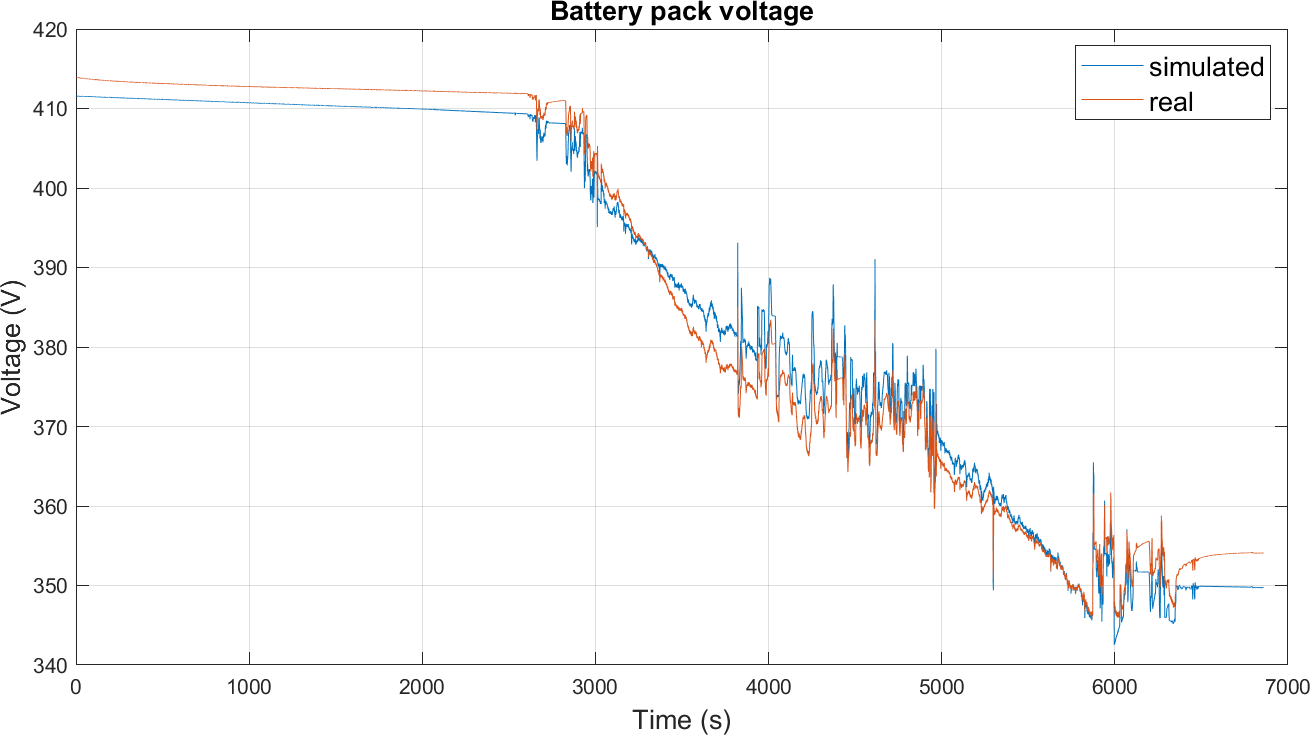
\includegraphics[width=\textwidth]{images/par_est_V_eup}
    \caption{e-up!}
\end{subfigure}

\vspace{20pt}

\begin{subfigure}{\textwidth}
    \centering
    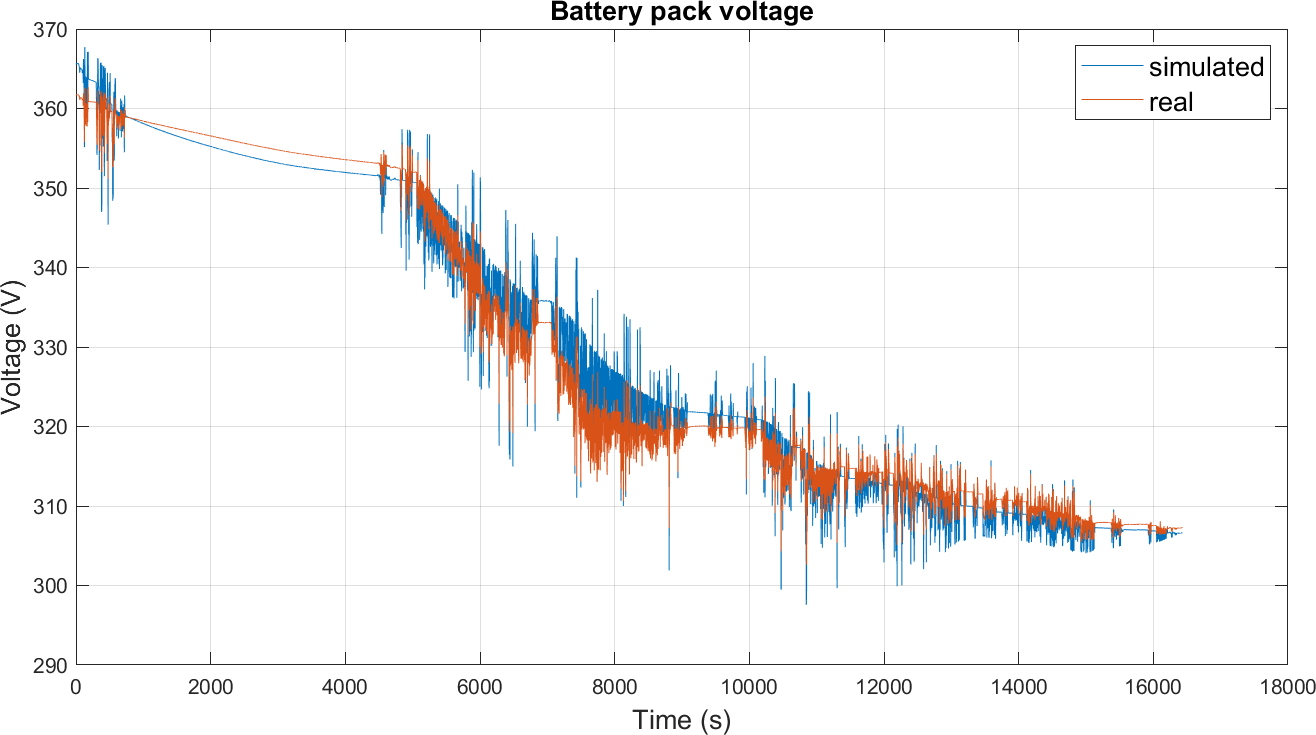
\includegraphics[width=\textwidth]{images/par_est_V_egolf}
    \caption{e-Golf}
\end{subfigure}
\caption[Simulated and real voltage signal after parameter estimation]{Simulated and real voltage signal after parameter estimation}
\label{fig:par_est_comparison_V}
\end{figure}

\begin{figure}[htbp!]
\centering
\begin{subfigure}{\textwidth}
    \centering
    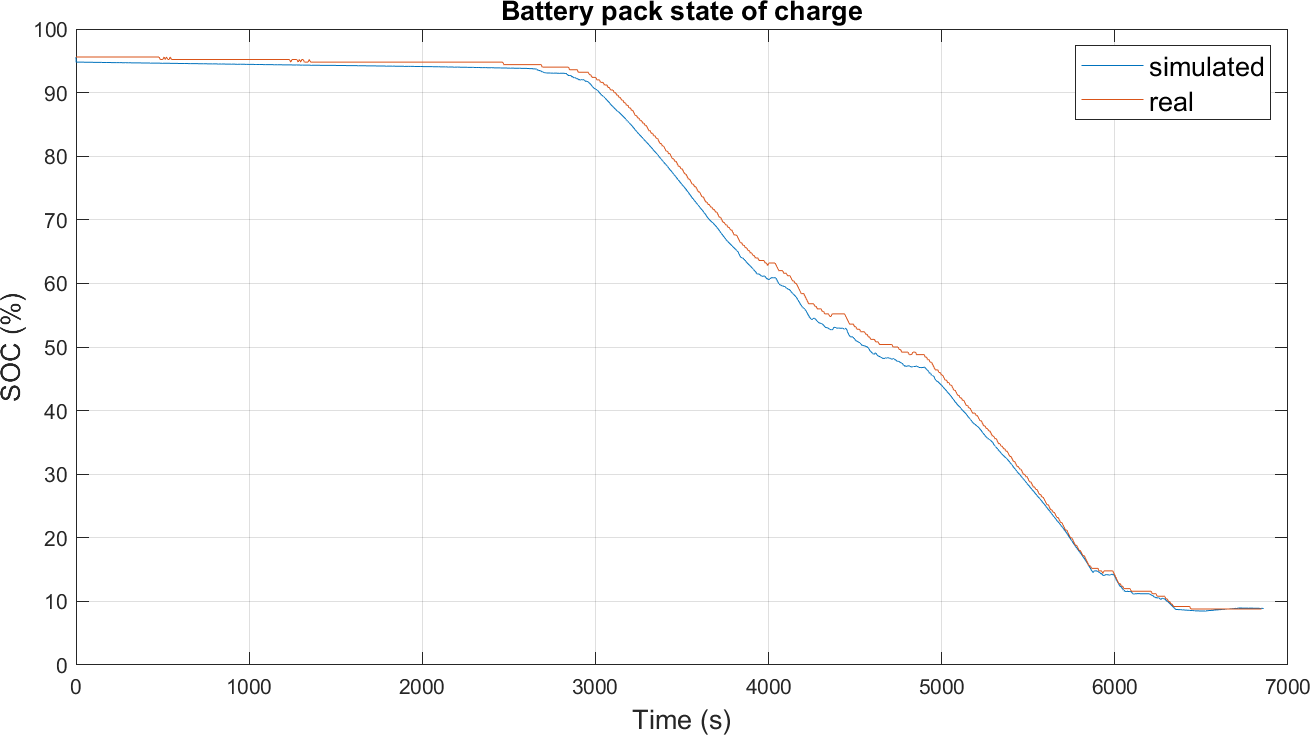
\includegraphics[width=\textwidth]{images/par_est_SOC_eup}
    \caption{e-up!}
\end{subfigure}

\vspace{20pt}

\begin{subfigure}{\textwidth}
    \centering
    \includegraphics[width=\textwidth]{images/par_est_SOC_egolf}
    \caption{e-Golf}
\end{subfigure}
\caption[Simulated and real SOC signal after parameter estimation]{Simulated and real SOC signal after parameter estimation}
\label{fig:par_est_comparison_SOC}
\end{figure}

As for the thermal model, the thermal resistance and thermal time constant have been estimated by trial and error. Namely, they were initialized to different values for many simulations, and the values for which the deviation between the simulated and real battery temperature was low enough were kept. Fig. \ref{fig:par_est_comparison_T} shows a comparison of the simulated temperature signal versus the experimental (real) one. The deviation between the simulated and real signal is very high at times, but the general trend of the real signal is mimicked successfully. We claim that this behaviour is due to the very low-complexity thermal model that the Simulink battery block implements (as discussed in sec. \ref{sec:known_limitations}).

\begin{figure}[htbp!]
\centering
\begin{subfigure}{\textwidth}
    \centering
    \includegraphics[width=\textwidth]{images/par_est_T_eup}
    \caption{e-up!}
\end{subfigure}

\vspace{20pt}

\begin{subfigure}{\textwidth}
    \centering
    \includegraphics[width=\textwidth]{images/par_est_T_egolf}
    \caption{e-Golf}
\end{subfigure}
\caption{Simulated vs real temperature signal after (manual) parameter estimation}
\label{fig:par_est_comparison_T}
\end{figure}





\section{EFC to SOH conversion}
\label{sec:efc2soh}
As discussed in sec. \ref{sec:soh}, there is no general mathematical relationship between the SOH and the number of EFC. The age of the generic battery model in Simulink can only be set as number of EFC; however, we are interested in expressing the age of the battery pack in terms of SOH.

To overcome this issue, we can set up a simple Simulink simulation which consists in imposing a constant 1C discharge current to the battery block (with an initial SOC of 100\%) and waiting for its complete discharge (SOC = 0\%). Then, the actual capacity of the battery is computed by simply multiplying the magnitude of the imposed discharge current and the ending time of the simulation (in hours). This capacity estimation technique is known as Coulomb counting (sec. \ref{sec:dmb_methods}). Finally, the SOH is obtained by dividing the result of the multiplication by the maximum theoretical capacity of the battery under nominal operating conditions (\texttt{maxCap}).

Since the battery pack aging model is parametrized in the same way for the e-up! and the e-Golf Simulink models, the EFC-to-SOH mapping is unique for the two models. The experiment has been performed 31 times, for EFC values ranging from 0 to 3000 with a step of 100. The resulting mapping is reported graphically in fig. \ref{fig:efc2soh}.

\begin{figure}[hbt!]
    \centering
    \includegraphics[width=0.75\textwidth]{images/efc2soh}
    \caption[EFC to SOH conversion]{EFC to SOH conversion (linearly interpolated)}
    \label{fig:efc2soh}
\end{figure}

It appears that Simulink's generic battery model is characterized by a linear relationship between EFC and SOH (as opposed to a generic real battery).






\section{Synthetic dataset generation}
\label{sec:ds_gen}
The parametrized EV model can now be used to generate a synthetic dataset of EV monitoring data. To simulate a single driving session, the user must specify a driving cycle, outside temperature [°C] (fixed or as a time series of measurements), initial average battery pack temperature [°C], initial battery pack SOC and battery pack SOH. The monitored signals are: speed [km/h], terminal voltage V [V], current I [A], SOC(\%), average battery internal temperature T [°C]. Additionally, the user can specify a specific \texttt{sampling\_rate} for the monitored signals (default is 0.2 s). Resampling through linear interpolation is performed at the end of each simulation on all the acquired signals according to the specified sampling rate, in order to achieve a common time base for all the signals. The choice of the sampling rate is a trade-off between computation time and signal fidelity: a fast sampling rate may capture high frequency changes in the signals more accurately, at the cost of a higher simulation time.

Since it is infeasible to acquire data for every possible combination of SOH, driving cycle, initial internal and external temperature, we design the following synthetic dataset generation procedure, with the aim of acquiring a minimal but sufficiently representative set of monitoring data in a very wide range of driving conditions:

\begin{algorithm}
\caption{Simulink EV model synthetic dataset generation}
\label{alg:ds_gen}
\begin{algorithmic}[1]
\For{\texttt{efc} $\in$ \texttt{EFC\_LEVELS}}
    \For{\texttt{dc} $\in$ \texttt{DC\_LIST}}
        \State $\text{\texttt{initSOC}} \gets \mathcal{U}(91,96)$
        \State $\text{\texttt{T\_outside}} \gets \mathcal{U}(-5,30)$
        \State $\text{\texttt{initBattTemp}} \gets \mathcal{U}(\text{\texttt{T\_outside}},\text{\texttt{T\_outside}}+5)$
        \State \textbf{simulate} \texttt{dc} in loop until $\text{SOC} < 10$
        \State get simulated signals (speed, V, I, SOC, T)
        \State resample signals every \texttt{sampling\_rate} s
        \State store dataset on disk
    \EndFor
\EndFor
\State concatenate datasets
\end{algorithmic}
\end{algorithm}

where "$\leftarrow\mathcal{U}(a,b)$" is a random extraction from the uniform distribution on $[a,b]$, \texttt{EFC\_LEVELS} is a list of EFC values at which to set the battery block for the simulation and \texttt{DC\_LIST} is a list of drive cycles that we wish to simulate.

To be representative, the synthetic dataset should contain driving session data associated to SOH values ranging from 100\% to 80\% (end of life); therefore we have set \texttt{EFC\_LEVELS} = [0, 100, 200, \dots, 2000] (since EFC = 2000 roughly corresponds to SOH = 80\%). Moreover, to span different driving conditions (city, urban and highway driving\footnote{We can categorize drive cycles in three categories: city (max speed <50 km/h), urban (max speed <90 km/h), highway (max speed >90 km/h).}), 12 standard drive cycles \cite{drive_cycles} have been included in \texttt{DC\_LIST}; they are listed in tab. \ref{tab:dc_list}. Additionally, we have also included three driving cycles (2x highway, 1x urban) extracted from the e-up! real dataset (chap. \ref{sec:aviloo_ds}), for a total of 15 drive cycles.

\begin{table}[htb!]
\centering
\begin{tabular}[t]{cc}
\toprule
Drive cycle name & Type\\
\midrule
Artemis Urban & city\\
Artemis Rural Road & urban\\
Artemis Motorway 130 kmph & highway\\
ECE R15 & city\\
EUDC & highway\\
FTP72 & urban\\
IM240 & urban\\
J1015 & city\\
LA92 & urban\\
NYCC & city\\
UDDS & urban\\
US06 & highway\\
\bottomrule
\end{tabular}
\caption[Selected standard drive cycles]{Standard drive cycles included in \texttt{DC\_LIST}.}
\label{tab:dc_list}
\end{table}

The dataset generation procedure has been run once for each EV model. Each of the two resulting datasets consists of a combination of 315 driving sessions, each associated to a specific (SOH, drive cycle) combination. There is no invalid or missing data. Before using these two synthetically generated datasets, they are further cleaned and preprocessed as explained in sec. \ref{sec:ds_preprocessing}.

% real dataset
\chapter{Real dataset}
\label{sec:aviloo_ds}

\section{Data acquisition}
\label{sec:aviloo_ds_intro}
To further expand our collection of EV monitoring data and in order to parametrize our Simulink EV model correctly (sec. \ref{sec:parameter_estimation}), two datasets of real EV field measurements were acquired from a private EV fleet management company (sec. \ref{sec:aviloo}). The datasets span several months of data acquisition from a VW e-up! and a VW e-Golf. Many battery SOH tests were performed throughout the monitored time periods, as reported in the next section.

\begin{figure}[htb!]
\centering
\begin{subfigure}[t]{0.475\textwidth}
    \centering
    \includegraphics[width=\textwidth]{images/eup}
    \caption{VW e-up!}
\end{subfigure}
\hfill
\begin{subfigure}[t]{0.475\textwidth}
    \centering
    \includegraphics[width=\textwidth]{images/egolf}
    \caption{VW e-Golf}
\end{subfigure}
\caption[VW e-up! and VW e-Golf]{The two Volkswagen EV models monitored by the private EV fleet management company.}
\label{fig:eup_egolf}
\end{figure}



\section{Data exploration}
\label{sec:aviloo_ds_exploration}
The two vehicles were monitored over different time periods\footnote{dates are in dd/mm/yyyy format}:
\begin{itemize}
    \item e-up!: 20/10/2021 - 18/12/2021
    \item e-Golf: 04/06/2019 - 12/06/2019, 27/06/2019 - 22/10/2020, 16/11/2020 - 07/12/2020, 15/02/2021 - 10/03/2021, 06/04/2021 - 10/05/2021, 12/07/2021 - 07/09/2021
\end{itemize}

Battery tests were performed over the monitored time periods for both models. The e-up! underwent a single battery test on 06/12/2021, which returned an SOH of 88\%. The e-Golf underwent 16 battery tests, whose dates and returned SOH values are reported in tab. \ref{tab:egolf_bchecks} for convenience.

\begin{table}[htb!]
\centering
\begin{tabular}[t]{cc}
\toprule
Test date & SOH(\%)\\
\midrule
22/07/2020 & 95\\
10/09/2020 & 95\\
23/11/2020 & 95\\
29/11/2020 & 93\\
17/02/2021 & 94*\\
08/03/2021 & 95\\
26/04/2021 & 95\\
03/05/2021 & 95\\
\bottomrule
\end{tabular}
\hspace{1cm}
\begin{tabular}[t]{cc}
\toprule
Test date & SOH(\%)\\
\midrule
08/07/2021 & 93\\
12/07/2021 & 95\\
16/08/2021 & 93\\
23/08/2021 & 95\\
15/09/2021 & $>100$*\\
02/11/2021 & 89*\\
05/11/2021 & 93*\\
22/11/2021 & 91*\\
\bottomrule
\end{tabular}
\caption[Battery tests performed on the monitored VW e-Golf]{Battery tests performed on the monitored VW e-Golf. Asterisk marks (*) indicate that the battery test doesn't fulfill the standard conditions for a reliable SOH estimation (i.e. driving the car from $100\%$ SOC to $<10\%$ SOC, as discussed in sec. \ref{sec:aviloo}), thus the estimated SOH value might not reflect the actual one precisely. The estimated SOH values have a maximum error of $\pm 1.5$, as claimed by the private EV fleet management company from whom the data was acquired.}
\label{tab:egolf_bchecks}
\end{table}

Training a machine learning algorithm for the real-time on-board SOH estimation requires having extensive monitoring data collected at different SOH levels. Unfortunately, the estimated SOH values during the monitored time periods exhibit very little variability. Therefore, e-up! and e-Golf real datasets will be used only for evaluating the performances of the proposed SOH estimation procedure (sec. \ref{sec:results}). To make the two datasets suitable for testing, only data of driving sessions associated to known battery test SOH values may be selected. We will make the assumption that data spanning from one week before and one week after a battery test (where available\footnote{As evident from tab. \ref{tab:egolf_bchecks}, there are some battery tests which were performed outside of the monitored time periods, therefore no monitoring data is available close in time to them}) is associated with the SOH value returned by that battery test. Whenever two contiguous battery tests were performed less than two weeks away from each other, less than a week of monitoring data is selected after or before those battery tests, in order to avoid any overlapping.

The provided monitoring data is characterized by many signals, whose measurements were collected by the BMS of the EV at different sampling rates and read by a monitoring device through the OBD port. The signals monitored by the BMS vary among different EV models; however, being designed from the same manufacturer, the VW e-up! and VW e-Golf have almost the same set of monitored signals. A complete list of all the common signals between the e-up! and the e-Golf is reported in tab. \ref{tab:aviloo_signals}.

\begin{table}[htb!]
\scriptsize
\centering
\begin{tabular}[t]{lll}
\toprule
Signal name & Description & \breakcellleft{Avg. sampling\\rate (s)}\\
\midrule
CUMULATIVE\_CC & Cumulative charged charge [C] & 33\\
CUMULATIVE\_CE & Cumulative charged energy [J] & 33\\
CUMULATIVE\_DC & Cumulative discharged charge [C] & 33\\
CUMULATIVE\_DE & Cumulative discharged energy [J] & 33\\
CURRENT & Current flowing through the pack [A] & 0.15, 0.1\\
ENERGY\_REMAINING\_EXPECTED & Remaining energy (expected) [J] & 23\\
IGNITION & Whether the vehicle is on (1) or off (0) & 7\\
MILEAGE & Mileage [km] & 17\\
SERIAL\_BATTERY & Serial number of the pack (string) & 100\\
SOC\_DISPLAY & Displayed SOC(\%) & 7\\
SOC\_REAL & Actual SOC(\%) & 7\\
SPEED & Speed [km/h] & 13, 19\\
T\_CELL\_AVG & Average cell temperature [°C] & 12\\
T\_CELL\_MAX & Maximum cell temperature [°C] & 12\\
T\_CELL\_MIN & Minimum cell temperature [°C] & 12\\
T\_MODULE\_$n$ & Temperature of the $n$-th module [°C] & 13, 4\\
T\_OUTSIDE & External temperature [°C] & 100, 14\\
VOLTAGE & Terminal voltage of the pack [V] & 0.15, 0.1\\
VOLTAGE\_12V & Terminal voltage of the ignition battery [V] & 21\\
VOLTAGE\_CELL\_$n$ & Terminal voltage of the $n$-th cell [V] & 1\\
VOLTAGE\_CELL\_MAX & Maximum cell terminal voltage [V] & 1\\
VOLTAGE\_CELL\_MAX\_NUMBER & Cell with the highest terminal voltage & 1\\
VOLTAGE\_CELL\_MIN & Minimum cell terminal voltage [V] & 1\\
VOLTAGE\_CELL\_MIN\_MUMBER & Cell with the lowest terminal voltage & 1\\
VOLTAGE\_CONN & Voltage at the connector [V] & 0.15, 0.1\\
\bottomrule
\end{tabular}
\caption[Signals monitored by the BMS]{Signals monitored by the BMS and read by a monitoring device through the OBD port. When sampling rates are different between the two models, the e-up! sampling time is reported first. In both datasets there is no invalid data; however "SPEED" measurements are missing in some e-Golf driving sessions.}
\label{tab:aviloo_signals}
\end{table}

The e-up! data was provided directly on a proprietary online platform, in a format which makes it easy to explore and manage the data. Data associated with each driving session can be selected and downloaded in csv format directly from the platform. On the other hand, the e-Golf data was provided in raw csv files, from which it was difficult to tell different driving sessions apart. Moreover, "SPEED" measurements are missing in some of these files. Therefore, in this case, driving sessions have been manually identified and extracted with the following procedure:
\begin{itemize}
    \item where the "SPEED" measurements are available, a driving session corresponds to the time interval from the first sampled non-zero speed value to the last one, with sub-intervals of at most five minutes in which speed may be zero.
    \item where the "SPEED" measurements are not available, a driving session corresponds to the time interval from the first increase in "MILEAGE" value to the last one, with sub-intervals of at most five minutes in which mileage may not increase.
\end{itemize}

\noindent The csv files containing driving session data have rows formatted as
\[
\text{\texttt{Timestamp, Timestamp (Unix Microseconds), Signal Type, Value}}
\]
For our aims, only "SPEED", "VOLTAGE", "CURRENT", "SOC\_REAL" and "TEMPERATURE" signals are selected. Specifically: "SPEED" is needed to add real drive cycles to \texttt{DC\_LIST} for the synthetic dataset generation (sec. \ref{sec:ds_gen}); "VOLTAGE", "CURRENT", "SOC\_REAL" and "TEMPERATURE" are needed to parametrize Simulink's GBM block (sec. \ref{sec:parameter_estimation}) and -- with the exception of "TEMPERATURE" -- to test the performances of the proposed SOH estimation procedure (chap. \ref{sec:experiments}). The resulting dataset of extracted driving sessions, each associated to a known SOH level, will undergo further cleaning and preprocessing steps in sec. \ref{sec:ds_preprocessing}.

At a later time, a further set of battery test field data for six different e-Golf vehicles became available, with associated SOH values: 93\%, 94\%, 99\%, 94\%, 96\%, 98\%. They were acquired as raw csv files and processed as already explained. Finally, they were concatenated to the existing e-Golf driving sessions dataset.

% experiments and results
\chapter{Experiments and results}
\label{sec:experiments}

In this chapter, several novel SOH estimation procedures are introduced, each consisting in a combination of one feature extraction method followed by one regression model. Synthetic and real datasets, described in chapters \ref{sec:ev_model_ds_gen} and \ref{sec:aviloo_ds} respectively, are used to train and validate regression models for the SOH estimation, and finally to test their performances.

\section{Data preprocessing}
\label{sec:ds_preprocessing}
Several preprocessing steps have been performed on the two datasets, before using them for training and testing purposes. The two preprocessing pipelines are described in the following sections.

\subsection{Synthetic dataset}
\label{sec:synth_preprocessing}
The two synthetic datasets generated in sec. \ref{sec:ds_gen} have been used to train the proposed SOH estimation procedures and to evaluate their performances. The following preprocessing steps have been performed on each driving session of the two datasets:
\begin{enumerate}
    \item Filter out signals other than voltage, current and SOC.
    \item Set the first voltage and SOC measurements by backward linear interpolation:
    \begin{align}
        \text{V}(0) &= \frac{\text{V}(t_2)-\text{V}(t_1)}{t_2-t_1}(-t_1)+\text{V}(t_1)\\
        \text{SOC}(0) &= \frac{\text{SOC}(t_2)-\text{SOC}(t_1)}{t_2-t_1}(-t_1)+\text{SOC}(t_1)
    \end{align}
    where $t_1$ and $t_2$ are respectively the second and third timestamp at which signals were sampled\footnote{we set $\text{\texttt{sampling\_rate}} = 0.2$ s, so $t_1=0.2$ s and $t_2=0.4$ s.\label{note:sampling_rate}}. This is done in order to address a bug in Simulink's GBM block (sec. \ref{sec:battery_pack}) which gives incorrect voltage and SOC measurements at the beginning of the simulation.
    \item Format data into a multi-index Pandas dataframe, attaching the SOH value associated to the current driving session and a short identifier for the name of the drive cycle.
\end{enumerate}
The preprocessed driving sessions are then concatenated into a single dataset. At this point, each dataset consists of 315 driving sessions from half an hour to several hours long.

Each driving session is then split up into several non-overlapping 5-minute-long time windows which inherit the SOH value associated to that session. The time window extraction algorithm is reported in appendix \ref{sec:tw_extr_alg}. A total of $10192$ time windows are extracted from the e-up! dataset, and a total of $24224$ from the e-Golf dataset. The data associated to each time window can be viewed as a multivariate time series with $C=3$ channels (V, I, SOC) and length $T=1500$ (i.e. 300 s $\times$ 5 measurements/s), therefore the resulting datasets of extracted time windows are time series datasets (def. \ref{def:ts_ds}) with $N_\text{e-up!}=10192$ and $N_\text{e-Golf}=24224$ samples respectively.

Since synthetic data will be used both for training regression models and testing them, each of the two time windows datasets is randomly split into a training set (80\% of the time windows) and a test set (20\%). Time windows are sampled in a stratified fashion, so that the distribution of different SOH levels in each subset is the same as in the original dataset.

Finally, standardization is applied to each signal, both in training and test set. Namely, the measurements $s_1,\dots,s_T$ of each signal are transformed to:
\begin{equation}
    z_i = \frac{s_i-\bar{\mathbf{s}}^\text{(train)}}{\hat{\sigma}_\mathbf{s}^\text{(train)}}
\label{eq:standardization}
\end{equation}
where $\bar{\mathbf{s}}^\text{(train)}$ and $\hat{\sigma}_\mathbf{s}^\text{(train)}$ are respectively the sample mean and sample standard deviation of the signal measurements in the training set. Computing the mean and standard deviation with respect to only the training set avoids data leakage from test data, which must be kept unseen until the end of the training phase.

We can convert each time series dataset to a static one by extracting relevant features from each time window. Feature extraction may be performed in a variety of ways, outlined in sec. \ref{sec:feature_extraction}.

\subsection{Real dataset}
\label{sec:aviloo_preprocessing}
Real field data (sec. \ref{sec:aviloo_ds_exploration}) has been used to evaluate the performances of the SOH estimation procedures, previously trained on synthetic data. The following preprocessing steps have been performed on each driving session of the two real datasets:
\begin{enumerate}
    \item Filter out signals other than voltage, current and SOC.
    \item Resample signals through linear interpolation with the same sampling rate specified for the synthetic dataset (sec. \ref{sec:ds_gen}). This is done in order to achieve a common time base for all signals.
    \item Format data into a multi-index Pandas dataframe, attaching the SOH value associated to the current driving session and a short identifier for the name of the drive cycle. Each signal will have its own column.
\end{enumerate}
The preprocessed driving sessions are concatenated into a single dataset. The synthetic and real datasets are now formatted all in the same way.

Time windows are then extracted from driving sessions, as already described in sec. \ref{sec:synth_preprocessing}. $N_\text{e-up!}=164$ and $N_\text{e-Golf}=1445$ samples are extracted in total. Similarly, signal standardization (eq. \ref{eq:standardization}) is applied at the end, reusing the already computed $\bar{\mathbf{s}}^\text{(train)}$ and $\hat{\sigma}_\mathbf{s}^\text{(train)}$. As already done for synthetic data, feature extraction is also performed on the two resulting real time windows datasets (sec. \ref{sec:feature_extraction}).

\section{Feature extraction}
\label{sec:feature_extraction}
Feature extraction provides a static representation for each time series dataset, making it easier to train regression models. To perform feature extraction, three approaches may be taken:
\begin{itemize}
    \item \textsc{MiniRocket}'s feature extraction for multivariate time series (sec. \ref{sec:multivariate-minirocket})
    \item OLS feature extraction (sec. \ref{sec:ols})
    \item Theil-Sen feature extraction (sec. \ref{sec:theil-sen})
\end{itemize}
Each approach has its pros and cons. \textsc{MiniRocket} extracts 9,996 features from each time series and is considered the state-of-the-art for TSER problems. However, it needs to be fit to training data in order to use it; moreover, its transform operation is computationally expensive, as almost 10,000 convolutions per time window need to be computed. OLS feature extraction\footnote{The key idea that motivates feature extraction based on OLS and Theil-Sen linear regression to time windows of EV monitoring data has been discussed in sec. \ref{sec:my_method}.\label{note:ols_ts_feat_extr}} generates 3 features per time series, does not need to be fit on training data and is computationally cheaper than \textsc{MiniRocket}. However, it is not robust to outliers in the V-I-SOC space. Theil-Sen feature extraction\footref{note:ols_ts_feat_extr} is similar to OLS, but is more robust to outliers. However, it is more computationally demanding than both OLS and \textsc{MiniRocket}.

Due to the huge number of features extracted by \textsc{MiniRocket}, PCA is applied to \textsc{MiniRocket}-transformed datasets. By visualizing the scree plot for the two synthetic training sets (fig. \ref{fig:scree_plot}), we observe that with just 32 features out of the original 9,996 we can explain over 90\% of the total variance in the data. A different PCA problem is solved for each of the two synthetic training sets. The first 32 principal components of the training sets are then used for all PCA transforms. Since PCA requires standardized data, time series data transformed through \textsc{MiniRocket} is standardized before the PCA transform\footnote{with sample mean and sample standard deviation defined by the synthetic training sets\label{note:pca_standardization}}. Furthermore, the PCA transform does not necessarily output standardized data, so standardization is applied also after every PCA transform\footref{note:pca_standardization}.

\begin{figure}[hbt!]
    \centering
    \includegraphics[width=\textwidth]{images/scree_plot}
    \caption[Scree plot for the \textsc{MiniRocket}-transformed e-Golf training set]{Scree plot for the \textsc{MiniRocket}-transformed e-Golf training set. The scree plot for the e-up! training set is very similar, thus it is not reported.}
    \label{fig:scree_plot}
\end{figure}




\section{Training regression models}
\label{sec:regr_model_training}
Several regression models can be selected for predicting the SOH from a transformed time window. In sec. \ref{sec:regr_models}, three models were discussed:
\begin{itemize}
    \item Ridge regression via SGD (RR, sec. \ref{sec:ridge})
    \item Random forest (RF, sec. \ref{sec:random_forest})
    \item Feed-forward neural network (NN, sec. \ref{sec:neural_network})
\end{itemize}
Three instances of each model are trained, one for each feature extraction method (for a total of 9 regression models per EV model). The training set used is the one introduced in sec. \ref{sec:synth_preprocessing}. Grid search with 5-fold cross-validation was performed to tune some of the hyperparameters of ridge regression and random forest models. The neural network hyperparameters were instead tuned by "trial and error", due to the higher computational cost of training such models; 10\% of the training set was set aside before training the neural network, to validate its performances at the end of each epoch. The optimal hyperparameters found are reported in appendix \ref{sec:hyperparameter tuning}. The workstation used to perform the training has the following specifications: Intel Xeon W-2155 CPU @ 3.30 GHz (10 cores, 20 threads), 64GB RAM, NVIDIA Quadro P4000 GPU (8GB GDDR5).

To speed up training, parallel computing has been performed by distributing operations across all the CPU cores available. Specifically, it has been applied during the cross-validation of ridge regression and random forest models.



\section{Performance evaluation}
\label{sec:results}
The trained regression models have been tested on the held out test sets of synthetic data and on the real datasets. The performances of each model are evaluated in terms of MAE (sec. \ref{sec:metrics}). For each feature extraction method the average feature extraction time is reported, as this metric is critical for a real-time SOH estimation procedure. Results are reported in tab. \ref{tab:results}.

\begin{table}[hbt!]
\centering
\begin{tabular}{rcccccccccl}
\toprule
& \phantom{} & \multicolumn{3}{c}{Synthetic} & \phantom{} & \multicolumn{3}{c}{Real} & \phantom{} & \\
\cmidrule{3-5} \cmidrule{7-9}
&& RR & RF & NN && RR & RF & NN && avg. time (s)\\
\midrule
\rule{0pt}{3ex}
\textbf{e-up!}\\
\cmidrule{1-1}
MR && 2.40 & 2.17 & 2.12 && 9.70 & 5.22 & 8.56 && 0.053\\
OLS && 4.28 & 0.90 & 1.36 && 5.10 & 5.70 & 10.67 && $1.9 \cdot 10^{-3}$\\
TS && 4.13 & 0.75 & 1.23 && 9.28 & 7.91 & 10.88 && 0.54\\
\rule{0pt}{5ex}
\textbf{e-Golf}\\
\cmidrule{1-1}
MR && 3.68 & 3.23 & 2.18 && 6.96 & 2.62 & 9.91 && 0.046\\
OLS && 4.37 & 2.36 & 2.91 && 5.23 & 5.56 & 7.81 && $1.8 \cdot 10^{-3}$\\
TS && 4.35 & 1.76 & 2.14 && 4.19 & 3.85 & 4.44 && 0.47\\
\bottomrule
\end{tabular}
\caption[Results of the experiments]{MAE of the SOH values predicted with the proposed regression procedures. Column names refer to regression models, row names refer to feature extraction methods. The last column is the average feature extraction time from a single time window.}
\label{tab:results}
\end{table}

All the feature extraction methods proposed are very fast to apply ($<1$ s per time window); the time for predicting the SOH value happens to be negligible ($<10^{-3}$ s per time window) for all regression models, thus it was not reported. We can therefore conclude that every possible combination of a single feature extraction method with a single regression model defines a SOH estimation procedure which fulfils the real-time requirement. We observe that RF+OLS and RF+TS perform very well on synthetic data. However, all regression procedures see a drastic decrease in performances when tested on field data from real EVs. It may seem that MR+RF is the best performing procedure for SOH estimation of real EVs, achieving a relatively low MAE of 2.36. However, the $R^2$ coefficient between the real and predicted SOH values is negative for all procedures applied on the real e-Golf dataset\footnote{whereas it doesn't make any mathematical sense to compute the $R^2$ in the case of the e-up! dataset, as the only represented SOH value is 0.88; see sec. \ref{sec:metrics}}, meaning that the average of the real SOH values is still a better estimator.

We claim that this underwhelming result may be attributed to the very nature of the available data, and not on the procedure itself. Specifically:
\begin{itemize}
    \item the key assumption made (namely that operating points lay on a 3D plane uniquely defined by the current SOH) may be accurate for synthetically generated data, but not enough for field data from a real EV. This would indicate that the EV Simulink model described in sec. \ref{sec:ev_model_ds_gen} is not sufficiently complex as to replicate the electrical and mechanical behavior of a real EV. In a sense, this problem is unavoidable: even if we made said Simulink model "richer" and closer to reality, we would have a hard time finding specific experimental data to parametrize it.
    \item the Simulink model may have overfit the experimental data used in the parameter estimation procedure (sec. \ref{sec:parameter_estimation}). Also in this case, the Simulink model may not replicate the behavior of a real EV accurately. To deal with this issue, we may repeat the parameter estimation using more battery test driving sessions.
    \item a higher amount and/or more diverse data is required to train the regression models. In this sense, we could generate more synthetic data in more varied driving conditions and check if retrained models give better SOH predictions.
\end{itemize}

Many possible enhancements exist, which could theoretically increase the performances of the novel SOH estimation procedure introduced in this work. They are investigated briefly in the final chapter, as a reference for potential future works.

\smallskip

An overview of the approach followed to train and test the proposed SOH estimation procedure is visualized in fig. \ref{fig:overview}.

\begin{figure}
    \centering
    \includegraphics[width=\textwidth]{images/schemone.pdf}
    \caption[Overview of the data pipeline designed to train and test the proposed SOH estimation procedure]{Overview of the data pipeline designed to train and test the proposed SOH estimation procedure.}
    \label{fig:overview}
\end{figure}

% conclusion and future works
\chapter{Conclusion}
\label{sec:conclusion}

In this work, a novel data-driven approach to Li-ion battery pack SOH estimation has been proposed. Due to a lack of publicly available datasets of EV field data, a Simulink model of an EV has been built and parametrized according to the technical specifications of two real EVs (VW e-up!, VW e-Golf). The model has been used to simulate a high number of driving sessions in different driving conditions, collecting synthetically-generated EV field data. Specifically, the resulting synthetic dataset consists of voltage, current and SOC measurements, recorded at a high sampling rate. Multiple fixed-length time windows were extracted from each synthetic driving session and three feature extraction methods (\textsc{MiniRocket}, OLS regression, Theil-Sen regression) were applied on them, thus obtaining a static representation of time series data. The transformed data was finally used to train three different regression models (ridge regression, random forest, feed-forward neural network).

The proposed procedure has been tested both on a held-out test set of synthetic data and on a real dataset of EV monitoring data, acquired from a private EV fleet management company. The models generally achieved a low MAE on synthetic data (as low as 0.75\%, obtained with Theil-Sen feature extraction followed by a random forest regression model). Moreover, the procedure has been shown to be very fast in making predictions (with at most half a second per time window), making it suitable for monitoring SOH in real-time. However, performances on real data were underwhelming. Supposedly, the poor generalization capabilities exhibited by the trained models are due to the low quantity, quality and/or diversity of the synthetically generated data, perhaps indicating that the Simulink EV model is not as close to reality as expected. Despite the promising results achieved on synthetic data, further work is needed to improve the performances of the proposed SOH estimation procedure on real EV data.

\section{Future work}
\label{sec:future_work}
Even though the performances of the procedure applied on real data were below expectations, we claim that there exist many possible improvements to our approach, which could theoretically enhance the regression models' generalization ability.

The main improvements regard the quantity, quality and diversity of the data used for training. Specifically, we may:
\begin{itemize}
    \item use the Simulink EV model to further generate synthetic data in more diverse driving conditions (e.g.: simulating more driving cycles and finer battery aging levels), thus increasing the size of the training set;
    \item increase the sampling rate. We used a sampling rate of 5 Hz (i.e. a measurement every 0.2 seconds), but higher sampling rates can be tested, enhancing the reliability of the measurements at the price of a higher computational cost for feature extraction;
    \item implement data augmentation techniques specific for time series data \cite{da_ts} to virtually increase the size of the training set;
    \item enhance the reliability of the Simulink EV model. For example, we could model the battery pack at the module or cell level (instead of approximating it to a single high-voltage battery cell), and we could explicitly implement the thermal management/cooling system of an EV (instead of relying on a simple battery thermal model). However, this is viable only upon acquiring more fine-grained EV specifications, such as the specific electrical and geometrical layout of the cells inside the battery pack, its positioning inside the car, the specific features of the BMS and of the battery thermal management system (BTMS) in use;
    \item improve the thermal model of the current Simulink EV model, so that the temperature dependence on the SOH is correctly accounted for. This improvement would make it possible to exploit also the extracted temperature measurements to predict SOH.
    \item train the regression models on a "hybrid" training set, composed of both synthetically-generated and real data.
    \item acquire new real data, over a wider time period (i.e. a higher amount of different SOH values between 100\% and 80\%). In fact, with a sufficiently extensive and representative amount of real data we could entirely avoid generating synthetic training data.
\end{itemize}

Moreover, also the proposed algorithms could be improved. We may:
\begin{itemize}
    \item extract longer time windows, in order to capture a wider set of operating points in different driving conditions. This comes at the cost of an increased computational time for applying feature extraction.
    \item with respect to the feature extraction method based on linear regression in the V-I-SOC space, experiment with different types of regression other than the linear one (e.g. Bayesian linear regression, polynomial regression).
    \item experiment with other regression models, such as support vector regression, Gaussian process regression and deep neural networks. Interestingly, there exist machine learning models which can at the same time learn how to extract relevant features from time series data and how to use them to perform extrinsic regression. Among them, a CNN known as InceptionTime \cite{inceptiontime, TSER} achieves state of the art performances on many TSER datasets. Using deep neural networks would also enable the use of transfer learning \cite{transferlearning}, a widely used methodology for increasing a model's generalization ability with just a little amount of target-domain data.
\end{itemize}

% THE END.


\appendix
% appendix
\newlength{\chaptertopskip}
\setlength{\chaptertopskip}{0pt}
\makeatletter
\xpatchcmd{\@makechapterhead}{\vspace*{50\p@}}{\vspace*{\chaptertopskip}}{\typeout{Success}}{\typeout{Failure!!!}}
\makeatother

\chapter{EV Simulink model - figures}
\label{appendix}



\rotatebox{90}{
\begin{minipage}{0.85\textheight}
    \includegraphics[width=\textwidth]{images/electricvehicle}
    \captionof{figure}{Simulink EV model}
    \label{fig:ev_model}
\end{minipage}
}
\hspace{3cm}
\rotatebox{90}{
\begin{minipage}{0.85\textheight}
    \includegraphics[width=\textwidth]{images/simulink_driver.pdf}
    \captionof{figure}{Simulink EV model - driver and braking subsystems}
    \label{fig:simulink_driver}
\end{minipage}
}

\newpage

\hspace{-1.5cm}
\rotatebox{90}{
\begin{minipage}{\textheight}
    \includegraphics[width=\textwidth]{images/simulink_battery.pdf}
    \captionof{figure}{Simulink EV model - battery pack subsystem}
    \label{fig:simulink_battery}
\end{minipage}
}
\hspace{2cm}
\rotatebox{90}{
\begin{minipage}{\textheight}
    \includegraphics[width=\textwidth]{images/simulink_drivetrain.pdf}
    \captionof{figure}{Simulink EV model - drivetrain subsystem}
    \label{fig:simulink_drivetrain}
\end{minipage}
}

\newpage

\begin{figure}[H]
    \centering
    \includegraphics[width=0.95\textwidth]{images/simulink_wheels.pdf}
    \caption{Simulink EV model - wheels subsystem}
    \label{fig:simulink_wheels}
\end{figure}

\begin{figure}[H]
    \centering
    \includegraphics[width=0.95\textwidth]{images/simulink_body.pdf}
    \caption{Simulink EV model - vehicle body subsystem}
    \label{fig:simulink_body}
\end{figure}







\chapter{Additional notes}

\section{Spatial median}
\label{sec:spatial_median}
Spatial medians are a family of multivariate medians, i.e. an extension of the notion of univariate median to multivariate distributions. Multiple Theil-Sen estimation (sec. \ref{sec:theil-sen}) uses a particular spatial median defined via a depth function, first introduced in \cite{spatial_median}.

Let $\mathbf{Z} \in \mathbb{R}^d$ be a random vector with joint probability distribution $Q$. The statistical spatial depth is defined as
\[
D_\text{sp}(\mathbf{z},Q) = 1 - \norm{\mathbb{E}_Q S(\mathbf{z}-\mathbf{Z})}, \qquad \mathbf{z} \in \mathbb{R}^d
\]
where $S(\mathbf{v})=\mathbf{v}/\norm{\mathbf{v}}$ $(S(\mathbf{0})=\mathbf{0})$ is the spatial sign function, i.e. the projection of $\mathbf{v} \in \mathbb{R}^k$ to a $k$-sphere.

For a random sample $\mathbf{Z_1},\dots,\mathbf{Z_n}$ drawn according to $Q$, the sample spatial depth is defined as
\[
\Tilde{D}_\text{sp}(\mathbf{z},Q_n) = 1 - \norm{\frac{1}{n} \sum_{i=1}^n S(\mathbf{z}-\mathbf{Z_i})}, \qquad \mathbf{z} \in \mathbb{R}^d
\]
where $Q_n$ is the empirical distribution over the random sample. Then, the statistical (sample) spatial median $m$ ($\Tilde{m}$) is the maximizer of the statistical (sample) spatial depth, i.e.
\[
m = \argsup_{x\in\mathbb{R}^d} D_\text{sp}(\mathbf{x},Q) \qquad\qquad \Tilde{m} = \argsup_{x\in\mathbb{R}^d} \Tilde{D}_\text{sp}(\mathbf{z},Q_n)
\]

\newpage

\section{Time windows extraction}
\label{sec:tw_extr_alg}
The algorithm for extracting time windows from a dataset of driving sessions' data is the following

\begin{algorithm}
\caption{Time windows extraction}
\label{alg:time_window_extraction}
\begin{algorithmic}[1]
\State \# \textbf{Input arguments}
\State \texttt{dataset}: the dataset from which to extract time windows
\State \texttt{length}: duration of the time windows [s] (default: 300)
\State \texttt{slide}: time between the starting points of two consecutive time windows [s] (default: \texttt{length}, i.e. non-overlapping time windows)
\State \texttt{freq}: sampling rate of the measurements [Hz] (default: 5)
\State \texttt{max\_SOC}: time windows do not contain SOC values above this one (default: 100)
\State \texttt{min\_SOC}: time windows do not contain SOC values under this one (default: 0)
\State \texttt{random\_starting\_point}: choose the starting point of the first time window at random in the interval $[0,\text{\texttt{length}}]$ (default: true)
\State 
\State \# \textbf{Function}
\State \texttt{time\_windows\_dataset} $\gets$ empty list
\For{driving session $\in$ \texttt{dataset}}
\State \texttt{duration} $\gets$ duration of the current driving session
    \If{\texttt{random\_starting\_point}}
        \State \texttt{start} $\gets$ $\mathcal{U}(0,\text{\texttt{length}})$
    \Else
        \State \texttt{start} $\gets$ 0
    \EndIf
    \State \texttt{end} $\gets$ $\text{\texttt{start}} + \text{\texttt{length}}$
    \While{\texttt{end} $\leq$ \texttt{duration}}
        \State \texttt{time\_window} $\gets$ $[\text{\texttt{start}},\text{\texttt{end}}]$
        \If{SOC values in \texttt{time\_window} are between \texttt{max\_SOC} and \texttt{min\_SOC}}
            \State append data of \texttt{time\_window} to \texttt{time\_windows\_dataset}
        \EndIf
        \State \texttt{start} $\gets$ \texttt{start} $+$ \texttt{slide}
        \State \texttt{end} $\gets$ \texttt{end} $+$ \texttt{slide}
    \EndWhile
\EndFor
\State \textbf{return} \texttt{time\_windows\_dataset}
\end{algorithmic}
\end{algorithm}



\section{Hyperparameter tuning}
\label{sec:hyperparameter tuning}
The hyperparameters chosen for each regression model are reported in the following table.

\begin{table}[hbt!]
\footnotesize
\centering
\rotatebox{90}{
\begin{minipage}{0.88\textheight}
%\ra{1.3} % 30% more space between rows
\begin{tabular}{rccccccccccccccccc}
\toprule
& \multicolumn{3}{c}{Ridge} & \phantom{} & \multicolumn{2}{c}{Random forest} & \phantom{} & \multicolumn{6}{c}{Neural network}\\
\cmidrule{2-4} \cmidrule{6-7} \cmidrule{9-14}
& $\alpha$ & $\eta_0$ & $p$ && \breakcell{max. tree\\depth} & n. trees && \breakcell{neurons\\per layer} & \breakcell{max.\\epochs} & $\alpha$ & $\eta_0$ & $\mu$ & $P$\\
\midrule
\rule{0pt}{3ex}
\textbf{e-up!}\\
\cmidrule{1-1}
\textsc{MiniRocket} & 0.0278 & 0.001 & 0.25 && 30 & 1000 && $(120, 60, 40)$ & 300 & 0.0001 & 0.1 & 0.9 & 5\\
OLS & 0.01 & 0.0464 & 0.25 && 50 & 500 && $(40, 20)$ & 300 & 0.0001 & 0.1 & 0.9 & 5\\
Theil-Sen & 0.01 & 0.0464 & 0.25 && unlimited & 500 && $(40, 20)$ & 300 & 0.0001 & 0.1 & 0.9 & 5\\
\rule{0pt}{5ex}
\textbf{e-Golf}\\
\cmidrule{1-1}
\textsc{MiniRocket} & 0.01 & 0.0008 & 0.25 && 30 & 1000 && $(120, 60, 40)$ & 300 & 0.0001 & 0.1 & 0.9 & 5\\
OLS & 0.01 & 0.0464 & 0.25 && 15 & 500 && $(40, 20)$ & 300 & 0.0001 & 0.1 & 0.9 & 5\\
Theil-Sen & 0.01 & 0.0464 & 0.25 && 15 & 500 && $(40, 20)$ & 300 & 0.0001 & 0.1 & 0.9 & 5\\
\bottomrule
\end{tabular}
\caption[Chosen hyperparameters]{Hyperparameters chosen for each regression model and training set. $\alpha$ is the regularization factor, $\eta_0$ is the initial learning rate. The ridge regression model is trained via SGD with learning rate computed at each iteration as $\eta(i) = \eta_0 / i^p$. The neural network is trained via SGD with learning rate divided by 10 whenever the training loss doesn't decrease enough for $P$ consecutive epochs.}
\end{minipage}}
\label{tab:hyperparameters}
\end{table}

% endnotes here if needed

\phantom{0}
\cleardoublepage

\printbibliography[heading=bibintoc] % heading required to show it in ToC

\end{document}
